\documentclass[12pt]{book}
\usepackage{geometry}         % See geometry.pdf to learn the layout options. There are lots.
\geometry{a4paper}            % ... or a4paper or a5paper or ...
%\geometry{landscape}         % Activate for rotated page geometry
\usepackage[parfill]{parskip} % Activate to begin paragraphs width empty line instead of indent
\usepackage{graphicx}
\usepackage{amssymb}
\usepackage{setspace}
\usepackage{amsmath}
\usepackage{url}
\usepackage{natbib}
\usepackage{pdfpages}
\usepackage{longtable}
\usepackage{booktabs}
\usepackage[]{hyperref}
\hypersetup{
    linktoc=all,
    colorlinks=true,
    citecolor=black,
    filecolor=black,
    linkcolor=black,
    urlcolor=blue
}


% The following specifies a line spacing of 1.2 times normal
\renewcommand{\baselinestretch}{1.2}

% Short-hand font settings used in this document:
\usepackage[T1]{fontenc}
\usepackage{lmodern}
\renewcommand\ttfamily{\usefont{T1}{lmtt}{m}{n}}
\newcommand{\term}[1]{{\bfseries\slshape #1}}
\newcommand{\ttt}[1]{\texttt{#1}}
\newcommand{\prout}[1]{\ttt{#1}}
\newcommand{\tb}[1]{\ttt{\textbf{#1}}}

%%%% JN: Draft version, February 2020
%%%% JN: I (JN) have started to review the text, and added occasional comments.
%%%% JN: Note that I use automatic text wrapping for paragraphs (in vim: `set textwidth=99`).

\begin{document}

\title{MrBayes version 3.2 Manual: \\ Tutorials and Model Summaries}

\date{\large Draft version, February 2020}

\author{Fredrik Ronquist, John P. Huelsenbeck, \\ Maxim Teslenko, Johan A. A. Nylander}

\maketitle

\tableofcontents

\newpage

\frontmatter

\chapter{Preface}
\label{preface}

When we started working on MrBayes in 1999-2000, we knew that there was a need for a Bayesian MCMC
package for phylogenetics, which was more flexible and easier to use than the software available
then. Nevertheless, we were astonished by how quickly users took MrBayes to their hearts. The
original release paper \citep{huelsenbeck01c}, which appeared in Bioinformatics in 2001, quickly
became a fast-track paper in Computer Science, as did the release note for version 3
\citep{ronquist03}, published in Bioinformatics in 2003. To date, these two papers have accumulated
more than 20,000 citations.

With the release of version 3.2 \citep{ronquist12a}, MrBayes has come of age. Through the years, we
have added to, extended, and rewritten the program to cover most of the models used in standard
statistical phylogenetic analyses today. We have also implemented a number of techniques to speed
up calculations, improve convergence, and facilitate Bayesian model averaging and model choice.
Version 3.2 has also undergone considerably more testing than previous versions of MrBayes. This
is not to say that MrBayes 3.2 is bug free but it should be considerably more stable than previous
versions. As in previous versions, we have done our best to document all of the available models
and tools in the online help and in this manual.

Version 3.2 of MrBayes also marks the end of the road for us in terms of major development.
Extending the original code has become increasingly difficult, and with version 3.2 we are at a
point where we feel we need to explore new approaches to Bayesian phylogenetics. Perhaps most
importantly, model specifications in MrBayes are strongly limited by the constraints of the Nexus
language. In a separate project, RevBayes, we hope to provide a generic computing environment that
allows users to build complex phylogenetic models interactively, from small building blocks.
However, such flexibility requires more of the user, and it may not be popular with everyone. For
standard analyses, MrBayes will remain adequate for years to come and it is our intention to
maintain the code base as long as the program remains heavily used and we have the resources to do
so.

The MrBayes project would not have been possible without the help from many people. First and
foremost, we would like to thank Maxim Teslenko, who has played an important role in fixing bugs
and adding functionality to MrBayes during the last couple of years. Among other things, Maxim is
responsible for a large part of the work involved in supporting BEAGLE, and in implementing the
stepping-stone method for estimating marginal likelihoods. Maxim has also contributed several
sections to this manual.

We are grateful for the financial support of the project provided by the Swedish Research Council,
the National Institutes of Health, and the National Science Foundation. We are also deeply indebted
to students, colleagues and numerous users of MrBayes, who have helped the project along in
important ways. We are not going to try to enumerate them here, as any attempt to do so is likely
to result in major omissions. However, we do want to express the overwhelming feeling of gratitude
we feel for the generosity with which people have shared ideas, bug fixes and other valuable tips
through the years. This feedback alone makes all the hours we have put into developing MrBayes
worthwhile. Thank you, all of you!

Last but not least, we would like to thank our families for the unwavering support they have
provided throughout the project. During intense programming periods, or when we have taught MrBayes
workshops around the world, they have had to cope with absent-minded fathers, aloof visitors, and
absent husbands. We realize that the childish enthusiasm we have shown when a new model resulted in
some incomprehensible numbers scrolling by on the screen has been poor compensation. Thank you so
much for all of your support and your sacrifices; we love you!

\flushleft November, 2011
\flushleft \textit{Fredrik Ronquist} \\
\textit{John Huelsenbeck}


\mainmatter

\chapter{Introduction}
\label{intro}
MrBayes 3 is a program for Bayesian inference and model choice across a large space of phylogenetic
and evolutionary models. The program has a command-line interface and should run on a variety of
computer platforms, including large computer clusters and multicore machines. Depending on the
settings, MrBayes analyses may demand a lot of your machine, both in terms of memory and processor
speed. Many users therefore run more challenging analyses on dedicated computing machines or
clusters. Several computing centers around the globe provide web access to such services. This
said, many standard analyses run fine on common desktop machines.

This manual explains how to use the program. After introducing you to the program in this chapter,
we first walk you through a simple analysis (chapter \ref{tutorialSimple}), which will get you
started, and a more complex partitioned analysis, which uses more of the program's capabilities
(chapter \ref{tutorialPartitioned}). This is followed by a set of shorter tutorials covering a
range of common types of analyses (chapter \ref{tutorialAdvanced}).

We then cover the capabilities of the program in more detail (chapter \ref{advancedTopics}),
followed by some details on the evolutionary models that are implemented (chapter
\ref{evolutionaryModels}). The manual ends with a series of diagrams giving a graphical overview of
the models and some proposal mechanisms implemented in the program (Appendix
\ref{appendixOverview}). For more detailed information about commands and options in MrBayes, see
the command reference that can either be downloaded from the program web site or generated from the
program itself (see section \ref{gettingHelp} below). All the information in the command reference
is also available on-line when using the program.

The manual assumes that you are familiar with the basic concepts of Bayesian phylogenetics. If you
are new to the subject, we recommend one of several recent reviews \citep{lewis01, holder03,
ronquist10}. The early papers introducing Bayesian phylogenetic methods \citep{li96, mau96,
rannala96, mau97, larget99, mau99, newton99} are also worthwhile reading. The basic MCMC techniques
are described in \citet{metropolis53} and \citet{hastings70}, and the Metropolis-coupled MCMC used
by MrBayes was introduced by \citet{geyer91}. Some recent general textbooks on Bayesian inference
and MCMC methods include \citet{gilks96a}, \citet{carlin00}, \citet{gelman03}, and
\citet{gamerman06}.


\section{Conventions Used in this Manual}

Throughout the document, we use \ttt{typewriter font} for things you see on screen or in a data
file, and \tb{bold typewriter font} for things you should type in. Alternative commands, options,
file names, etc are also given in \ttt{typewriter font}.

\section{Acquiring and Installing MrBayes}

MrBayes 3 is distributed without charge by download from the MrBayes web site,
\url{http://mrbayes.net}, or from the linked code repository on GitHub
\url{https://github.com/NBISweden/MrBayes}. If someone has given you a copy of MrBayes 3, we
strongly suggest that you download the most recent version from the official MrBayes site. The site
also gives detailed information about installation on different platforms (Window, Macintosh, Unix)
and describes how you can report bugs or contribute to the project.

MrBayes 3 is a plain-vanilla program that uses a command line interface and therefore behaves
virtually the same on all platforms --- Macintosh, Windows and Unix. Perhaps the easiest way of
installing the program is to compile it from source code in a Unix environment, as described in the
\ttt{README} and \ttt{INSTALL} documents in the MrBayes repository. The program may also be
available as binaries that run on Windows or Macintosh computers.

MrBayes comes with reasonably fast code for computing likelihoods, partly implemented using
so-called SIMD (single instruction, multiple data) technologies like SSE, AVX and FMA. However,
MrBayes will run faster with the specialized BEAGLE library \citep{ayres12}, which makes even
better use of the available computing resources. For instance, BEAGLE allows you to take advantage
of the processing power of your graphics card, which the standard MrBayes code does not. Installing
the BEAGLE library and linking it to MrBayes can be challenging; please follow the instructions in
the \ttt{INSTALL} file.

MrBayes is available both in a serial version and in a parallel version that uses MPI (message
passing interface) instructions to distribute computations across several processors or processor
cores. The serial version does not support multithreading, which means that you will not be able to
utilize more than one core on a multi-core machine for a single MrBayes analysis. If you want to
utilize all cores, you need to run the MPI version of MrBayes. The MPI version must be compiled
from source and will only run under Unix/Linux. Most Windows machines allow you to install a
parallel Linux partition, and all Macintosh computers come with a Unix system under the hood, which
will support MPI. Refer to the \ttt{README} and \ttt{INSTALL} documents for further instructions on
how to compile and run the MPI version.

The MrBayes package comes with example data files. These are intended to show various types of
analyses you can perform with the program, and you can use them as templates for your own analyses.
In the tutorials given in chapters \ref{tutorialSimple} to \ref{tutorialAdvanced}, you can learn
more about how to set up various types of analyses based on these example data files.

\section{Getting Started}

Start MrBayes by double-clicking the application icon (or typing \tb{./mb} or simply \tb{mb}
depending on your system) and you will see the information below:

\begin{singlespacing}
\footnotesize
\begin{verbatim}
                         MrBayes v3.2.7

                (Bayesian Analysis of Phylogeny)

        Distributed under the GNU General Public License


         Type "help" or "help <command>" for information
               on the commands that are available.

             Type "about" for authorship and general
                 information about the program.


   MrBayes >
\end{verbatim}
\normalsize
\end{singlespacing}

Note the \ttt{MrBayes >} prompt at the bottom, which tells you that MrBayes is ready for your
commands.

\subsubsection{Changing the Size of the MrBayes Window}

Some MrBayes commands will output a lot of information and write fairly long lines, so you may want
to change the size of the MrBayes window to make it easier to read the output. On Macintosh and
Unix machines, you should be able to increase the window size simply by dragging the margins. On a
Windows machine, you cannot increase the size of the window beyond the preset value by simply
dragging the margins but you can change both the size of the screen buffer and the console window
by right-clicking on the title bar of the MrBayes window and then selecting ``Properties'' in the
menu that appears. Make sure the ``Layout'' tab is selected in the window that appears, and then
set the ``Screen Buffer Size'' and ``Window Size'' to the desired values.

\section{Getting Help}
\label{gettingHelp}

At the \ttt{MrBayes >} prompt, type \tb{help} to see a list of the commands available in MrBayes.
Most commands allow you to set values (options) for different parameters. If you type \tb{help
<command>}, where \ttt{<command>} is any of the listed commands, you will see the help information
for that command as well as a description of the available options. For most commands, you will
also see a list of the current settings at the end. Try, for instance, \tb{help lset} or \tb{help
mcmc}. The \ttt{lset} settings table at the end should look like this:

\begin{singlespacing}
\footnotesize
\begin{verbatim}
   Parameter    Options                               Current Setting
   ------------------------------------------------------------------
   Nucmodel     4by4/Doublet/Codon/Protein              4by4
   Nst          1/2/6/Mixed                             1
   Code         Universal/Vertmt/Invermt/Yeast/Mycoplasma/
                Ciliate/Echinoderm/Euplotid/Metmt       Universal
   Ploidy       Haploid/Diploid/Zlinked                 Diploid
   Rates        Equal/Gamma/LNorm/Propinv/
                Invgamma/Adgamma/Kmixture               Equal
   Ngammacat    <number>                                4
   Nlnormcat    <number>                                4
   Nmixtcat     <number>                                4
   Nbetacat     <number>                                5
   Omegavar     Equal/Ny98/M3                           Equal
   Covarion     No/Yes                                  No
   Coding       All/Variable/Informative/Nosingletons
                Noabsencesites/Nopresencesites/
                Nosingletonabsence/Nosingletonpresence  All
   Parsmodel    No/Yes                                  No

   ------------------------------------------------------------------
\end{verbatim}
\normalsize
\end{singlespacing}

Note that MrBayes 3 supports abbreviations of commands and options, so in many cases it is
sufficient to type the first few letters of a command or option instead of the full name.

A complete list of commands and options can be generated as an ASCII text file by giving the
command \ttt{manual} to MrBayes. See the output of the command \tb{help manual} for more
information.

\section{Reporting and Fixing Bugs}

If you find a bug in MrBayes, we are grateful if you tell us about it using the bug reporting
functions of GitHub, as explained on the MrBayes web site (\url{www.mrbayes.net}).
%%%% JN: Remove or rewrite next paragraph. At least refer to direct contributions through github
Advanced users may be interested in fixing bugs themselves in the source code. Refer to section
\ref{advancedTopics} of this manual for information on how to contribute bug fixes, improved
algorithms or expanded functionality to other users of MrBayes.

\section{License and Warranty}

MrBayes is free software; you can redistribute it and/or modify it under the terms of the GNU
General Public License as published by the Free Software Foundation; either version 3 of the
License, or (at your option) any later version.

The program is distributed in the hope that it will be useful, but WITHOUT ANY WARRANTY; without
even the implied warranty of MERCHANTABILITY or FITNESS FOR A PARTICULAR PURPOSE. See the GNU
General Public License for more details (\url{http://www.gnu.org/copyleft/gpl.html}).

\section{Citing the Program}

If you wish to cite the program, you can simply refer to the most recent release note
\citep{ronquist12b}. That is,

\begin{singlespacing}
\footnotesize
Ronquist, F., M. Teslenko, P. van der Mark, D. Ayres, A. Darling, S. H\"{o}hna,
B. Larget, L. Liu, M. A. Suchard, and J. P. Huelsenbeck. 2012. MrBayes 3.2:
efficient Bayesian phylogenetic inference and model choice across a large model
space. Systematic Biology 61:539--542.
\normalsize
\end{singlespacing}

This manual should be cited as an online publication, for example:

\begin{singlespacing}
\footnotesize
Ronquist, F., J. P. Huelsenbeck, M. Teslenko, and J. A. A Nylander (2019) MrBayes version 3.2 manual:
tutorials and model summaries. Distributed with the software from
\url{https://github.com/NBISweden/MrBayes}
\normalsize
\end{singlespacing}

For more tips on citations, you can run the \ttt{citations} command in the program, which will give
you a number of other relevant citations for the program and its models and algorithms.


\chapter{Tutorial: A Simple Analysis}
\label{tutorialSimple}
This section walks you through a simple MrBayes example analysis to get you started. It is based on
the \ttt{primates.nex} data file and will guide you through a basic Bayesian MCMC analysis of
phylogeny, explaining the most important features of the program. There are two versions of the
tutorial. You will first find a Quick-Start version for impatient users who want to get an analysis
started immediately. The rest of the section contains a much more detailed description of the same
analysis.

\section{Quick Start Version}

There are four steps to a typical Bayesian phylogenetic analysis using MrBayes:
\begin{enumerate}
\item Read the Nexus data file
\item Set the evolutionary model
\item Run the analysis
\item Summarize the samples
\end{enumerate}

In more detail, each of these steps is performed as described in the following paragraphs:

\tb{1}. At the \ttt{MrBayes >} prompt, type \tb{execute primates.nex}. This will bring the data
into the program. When you only give the data file name (\ttt{primates.nex}), MrBayes assumes that
the file is in the current directory. If this is not the case, you have to use the full or relative
path to your data file, for example \ttt{execute ../examples/primates.nex}. If you are running your
own data file for this tutorial, beware that it may contain some MrBayes commands that can change
the behavior of the program; delete those commands or put them in square brackets to follow this
tutorial.

\tb{2}. At the \ttt{MrBayes >} prompt, type \tb{lset nst=6 rates=invgamma}. This sets the
evolutionary model to the GTR substitution model with gamma-distributed rate variation across sites
and a proportion of invariable sites (``GTR + I + $\Gamma$''). If your data are not DNA or RNA, if you
want to invoke a different model, or if you want to use non-default priors, refer to the rest of
this manual and the Appendix for more help.

\tb{3.1}. At the \ttt{MrBayes >} prompt, type \tb{mcmc ngen=20000 samplefreq=100 printfreq=100
diagnfreq=1000}. This will start the Markov chain Monte Carlo simulation. It will also ensure that
you get at least 200 samples from the posterior probability distribution, and that diagnostics are
calculated every 1,000 generations. For larger data sets you probably want to run the analysis
longer and sample less frequently. The default sample and print frequency is 500, the default
diagnostic frequency is 5,000, and the default run length is 1,000,000. You can find the predicted
remaining time to completion of the analysis in the last column printed to screen.

\tb{3.2}. If the standard deviation of split frequencies is below $0.01$ after 20,000 generations,
stop the run by answering \tb{no} when the program asks \ttt{Continue the analysis? (yes/no)}.
Otherwise, keep adding generations until the value falls below $0.01$. If you are interested mainly
in the well-supported parts of the tree, a standard deviation below $0.05$ may be adequate.

\tb{4.1}. Type \tb{sump} to summarize the parameter values using the same burn-in as the
diagnostics in the \ttt{mcmc} command. The program will output a table with summaries of the
samples of the substitution model parameters, including the mean, mode, and 95 \% credibility
interval (region of Highest Posterior Density, HPD) of each parameter. Make sure that the potential
scale reduction factor (PSRF) is reasonably close to $1.0$ for all parameters; if not, you need to
run the analysis longer. The same applies for the effective sample size (ESS). If the ESSs are
somewhere below 100, you may want to run longer.

\tb{4.2}. Summarize the trees using the same burn-in as the \ttt{mcmc} command by typing \tb{sumt}.
The program will output a cladogram with the posterior probabilities for each split and a phylogram
with mean branch lengths. Both trees will also be printed to a file that can be read by FigTree
\citep{rambaut12} and other tree-drawing programs, such as TreeView \citep{page96} and Mesquite
\citep{maddison06}.

It does not have to be more complicated than this; however, as you get more proficient you will
probably want to know more about what is happening behind the scenes. The rest of this section
explains each of the steps in more detail and introduces you to all the implicit assumptions you
are making and the machinery that MrBayes uses in order to perform your analysis.

\section{Thorough Version}

\subsection{Getting Data into MrBayes}

To get data into MrBayes, you need a so-called Nexus file that contains aligned nucleotide or amino
acid sequences, morphological (``standard'') data, restriction site (binary) data, or any mix of
these four data types. The Nexus data file is often generated by another program, such as Mesquite
\citep{maddison06}. Note, however, that MrBayes version 3 does not support the full Nexus standard,
so you may have to do a little editing of the file for MrBayes to process it properly. In
particular, MrBayes uses a fixed set of symbols~\footnote{The supported symbols are \{A, C, G, T, R, 
Y, M, K, S, W, H, B, V, D, N\} for DNA data, \{A, C, G, U, R, Y, M, K, S, W, H, B, V, D, N\} for RNA 
data, \{A, R, N, D, C, Q, E, G, H, I, L, K, M, F, P, S, T, W, Y, V, X\} for protein data, \{0, 1\} 
for restriction (binary) data, and \{0, 1, 2, 3, 4, 5, 6, 5, 7, 8, 9\} for standard (morphology) 
data.} for each data type and does not support user-defined symbols. 

In addition to the standard one-letter ambiguity symbols for DNA and RNA listed above, ambiguity
can also be expressed using the Nexus parenthesis notation. For instance, if there is uncertainty
whether a taxon have state 2 or 3 for a specific character, it can be coded as (23) (or (2,3)).
The Nexus format also allows coding taxa as polymorphic --- where a taxon truly have both character
states 2 and 3. One would then use braces instead of paranthesis: \{23\}. MrBayes, however, does
not make any distinction between polymorphic states or uncertainty in states, but treat them the
same way (as uncertainty), so it does not matter whether you use parentheses or braces.

If you have other symbols in your matrix than the ones supported by MrBayes, you need to replace
them before processing the \ttt{DATA} block in MrBayes. You also need to remove the \ttt{Equate}
and \ttt{Symbols} statements in the \ttt{Format} line if they are included. Unlike the Nexus
standard, MrBayes supports data blocks that contain mixed data types as described in the tutorial
in chapter \ref{tutorialPartitioned}.

To put the data into MrBayes type \tb{execute $<$filename$>$} at the \ttt{MrBayes >} prompt, where
\tb{$<$filename$>$} is the name of the input file. To process our example file, type \tb{execute
primates.nex} or simply \tb{exe primates.nex} to save some typing (MrBayes allows you to use the
shortest unambiguous version of a command). Note that the input file must be located in the same
folder (directory) where you started the MrBayes application (or else you will have to give the
path to the file) and the name of the input file should not have blank spaces, or it will have to
be quoted. If everything proceeds normally, MrBayes will acknowledge that it has read the data in
the \ttt{DATA} block of the Nexus file by outputting some information about the file read in.

\subsection{Specifying a Model}

All of the commands are entered at the \ttt{MrBayes >} prompt. At a minimum two commands,
\ttt{lset} and \ttt{prset}, are required to specify the evolutionary model that will be used in the
analysis. Usually, it is also a good idea to check the model settings prior to the analysis using
the \ttt{showmodel} command. In general, \ttt{lset} is used to define the structure of the model
and \ttt{prset} is used to define the prior probability distributions on the parameters of the
model. In the following, we will specify a GTR + I + $\Gamma$ model (a General Time Reversible model
with a proportion of invariable sites and a gamma-shaped distribution of rates across sites) for
the evolution of the mitochondrial sequences and we will check all of the relevant priors. We
assume that you are familiar with the common stochastic models of molecular evolution.

In general, a good start is to type \tb{help lset}. Ignore the help information for now and
concentrate on the table at the bottom of the output, which specifies the current settings. It
should look like this:

\begin{singlespacing}
\footnotesize
\begin{verbatim}
   Model settings for partition 1:

   Parameter    Options                               Current Setting
   ------------------------------------------------------------------
   Nucmodel     4by4/Doublet/Codon/Protein              4by4
   Nst          1/2/6/Mixed                             1
   Code         Universal/Vertmt/Invermt/Yeast/Mycoplasma/
                Ciliate/Echinoderm/Euplotid/Metmt       Universal
   Ploidy       Haploid/Diploid/Zlinked                 Diploid
   Rates        Equal/Gamma/LNorm/Propinv/
                Invgamma/Adgamma/Kmixture               Equal
   Ngammacat    <number>                                4
   Nlnormcat    <number>                                4
   Nmixtcat     <number>                                4
   Nbetacat     <number>                                5
   Omegavar     Equal/Ny98/M3                           Equal
   Covarion     No/Yes                                  No
   Coding       All/Variable/Informative/Nosingletons
                Noabsencesites/Nopresencesites/
                Nosingletonabsence/Nosingletonpresence  All
   Parsmodel    No/Yes                                  No

   ------------------------------------------------------------------
\end{verbatim}
\normalsize
\end{singlespacing}

First, note that the table is headed by \ttt{Model settings for partition 1}. By default, MrBayes
divides the data into one partition for each type of data you have in your \ttt{DATA} block. If you
have only one type of data, all data will be in a single partition by default. How to change the
partitioning of the data will be explained in the tutorial in chapter \ref{tutorialPartitioned}.

The \ttt{Nucmodel} setting allows you to specify the general type of DNA model. The \ttt{Doublet}
option is for the analysis of paired stem regions of ribosomal DNA and the \ttt{Codon} option is
for analyzing the DNA sequence in terms of its codons. We will analyze the data using a standard
nucleotide substitution model, in which case the default \ttt{4by4} option is appropriate, so we
will leave \ttt{Nucmodel} at its default setting.

The general structure of the substitution model is determined by the \ttt{Nst} setting. By default,
all substitutions have the same rate (\ttt{Nst=1}), corresponding to the F81 model (or the JC model
if the stationary state frequencies are forced to be equal using the \ttt{prset} command, see
below). We want the GTR model (\ttt{Nst=6}) instead of the F81 model so we type \tb{lset nst=6}.
MrBayes should acknowledge that it has changed the model settings.

The \ttt{Code} setting is only relevant if the \ttt{Nucmodel} is set to \ttt{Codon}. The
\ttt{Ploidy} setting is also irrelevant for us. However, we need to change the \ttt{Rates} setting
from the default \ttt{Equal} (no rate variation across sites) to \ttt{Invgamma} (gamma-shaped rate
variation with a proportion of invariable sites). Do this by typing \tb{lset rates=invgamma}.
Again, MrBayes will acknowledge that it has changed the settings. We could have changed both
\ttt{lset} settings at once if we had typed \tb{lset nst=6 rates=invgamma} in a single line.

We will leave the \ttt{Ngammacat} setting (the number of discrete categories used to approximate
the gamma distribution) at the default of 4. In most cases, four rate categories are sufficient. It
is possible to increase the accuracy of the likelihood calculations by increasing the number of
rate categories. However, the time it will take to complete the analysis will increase in direct
proportion to the number of rate categories you use, and the effects on the results will be
negligible in most cases.

Of the remaining settings, it is only \ttt{Covarion} and \ttt{Parsmodel} that are relevant for
single nucleotide models. We will use neither the parsimony model nor the covariotide model for our
data, so we will leave these settings at their default values. If you type \tb{help lset} now to
verify that the model is correctly set, the table should look like this:

\begin{singlespacing}
\footnotesize
\begin{verbatim}
   Model settings for partition 1:

   Parameter    Options                               Current Setting
   ------------------------------------------------------------------
   Nucmodel     4by4/Doublet/Codon/Protein              4by4
   Nst          1/2/6/Mixed                             6
   Code         Universal/Vertmt/Invermt/Yeast/Mycoplasma/
                Ciliate/Echinoderm/Euplotid/Metmt       Universal
   Ploidy       Haploid/Diploid/Zlinked                 Diploid
   Rates        Equal/Gamma/LNorm/Propinv/
                Invgamma/Adgamma/Kmixture               Invgamma
   Ngammacat    <number>                                4
   Nlnormcat    <number>                                4
   Nmixtcat     <number>                                4
   Nbetacat     <number>                                5
   Omegavar     Equal/Ny98/M3                           Equal
   Covarion     No/Yes                                  No
   Coding       All/Variable/Informative/Nosingletons
                Noabsencesites/Nopresencesites/
                Nosingletonabsence/Nosingletonpresence  All
   Parsmodel    No/Yes                                  No

   ------------------------------------------------------------------
\end{verbatim}
\normalsize
\end{singlespacing}

\subsection{Setting the Priors}

We now need to set the priors for our model. There are six types of parameters in the model: the
topology, the branch lengths, the four stationary frequencies of the nucleotides, the six different
nucleotide substitution rates, the proportion of invariable sites, and the shape parameter of the
gamma distribution of rate variation. The default priors in MrBayes work well for most analyses,
and we will not change any of them for now. By typing \tb{help prset} you can obtain a list of the
default settings for the parameters in your model. The table at the end of the help information
reads:

\begin{singlespacing}
\scriptsize
\begin{verbatim}
   Model settings for partition 1:
   Parameter        Options                      Current Setting
   ------------------------------------------------------------------
   Tratiopr         Beta/Fixed                   Beta(1.0,1.0)
   Revmatpr         Dirichlet/Fixed              Dirichlet(1.0,1.0,1.0,1.0,1.0,1.0)
   Aamodelpr        Fixed/Mixed                  Fixed(Poisson)
   Aarevmatpr       Dirichlet/Fixed              Dirichlet(1.0,1.0,...)
   Omegapr          Dirichlet/Fixed              Dirichlet(1.0,1.0)
   Ny98omega1pr     Beta/Fixed                   Beta(1.0,1.0)
   Ny98omega3pr     Uniform/Exponential/Fixed    Exponential(1.0)
   M3omegapr        Exponential/Fixed            Exponential
   Codoncatfreqs    Dirichlet/Fixed              Dirichlet(1.0,1.0,1.0)
   Statefreqpr      Dirichlet/Fixed              Dirichlet(1.0,1.0,1.0,1.0)
   Shapepr          Uniform/Exponential/Fixed    Exponential(1.0)
   Ratecorrpr       Uniform/Fixed                Uniform(-1.0,1.0)
   Pinvarpr         Uniform/Fixed                Uniform(0.0,1.0)
   Covswitchpr      Uniform/Exponential/Fixed    Uniform(0.0,100.0)
   Symdirihyperpr   Uniform/Exponential/Fixed    Fixed(Infinity)
   Topologypr       Uniform/Constraints/Fixed/   Uniform
                    Speciestree
   Brlenspr         Unconstrained/Clock/Fixed    Unconstrained:GammaDir(1.0,0.100,1.0,1.0)
   Treeagepr        Gamma/Uniform/Fixed/         Gamma(1.00,1.00)
                    Truncatednormal/Lognormal/
                    Offsetlognormal/Offsetgamma/
                    Offsetexponential
   Speciationpr     Uniform/Exponential/Fixed    Exponential(10.0)
   Extinctionpr     Beta/Fixed                   Beta(1.0,1.0)
   Fossilizationpr  Beta/Fixed                   Beta(1.0,1.0)
   SampleStrat      Random/Diversity/Cluster/    Random
                    FossilTip
   Sampleprob       <number>                     1.00000000
   Popsizepr        Lognormal/Gamma/Uniform/     Gamma(1.0,10.0)
                    Normal/Fixed
   Popvarpr         Equal/Variable               Equal
   Nodeagepr        Unconstrained/Calibrated     Unconstrained
   Clockratepr      Fixed/Normal/Lognormal/      Fixed(1.00)
                    Exponential/Gamma
   Clockvarpr       Strict/Cpp/TK02/Igr/Mixed    Strict
   Cppratepr        Fixed/Exponential            Exponential(0.10)
   Cppmultdevpr     Fixed                        Fixed(0.40)
   TK02varpr        Fixed/Exponential/Uniform    Exponential(1.00)
   Igrvarpr         Fixed/Exponential/Uniform    Exponential(10.00)
   Ratepr           Fixed/Variable=Dirichlet     Fixed
   Generatepr       Fixed/Variable=Dirichlet     Fixed

   ------------------------------------------------------------------
\end{verbatim}
\normalsize
\end{singlespacing}

We need to focus on \ttt{Revmatpr} (for the six substitution rates of the GTR rate matrix),
\ttt{Statefreqpr} (for the stationary nucleotide frequencies of the GTR rate matrix), \ttt{Shapepr}
(for the shape parameter of the gamma distribution of rate variation), \ttt{Pinvarpr} (for the
proportion of invariable sites), \ttt{Topologypr} (for the topology), and \ttt{Brlenspr} (for the
branch lengths).

The default prior probability density is a flat Dirichlet (all values are $1.0$) for both
\ttt{Revmatpr} and \ttt{Statefreqpr}. This is appropriate if we want estimate these parameters from
the data assuming no prior knowledge about their values. It is possible to fix the rates and
nucleotide frequencies but this is generally not recommended. However, it is occasionally necessary
to fix the nucleotide frequencies to be equal, for instance in specifying the JC and SYM models.
This would be achieved by using \ttt{prset statefreqpr=fixed(equal)}.

If we wanted to specify a prior that put more emphasis on equal nucleotide frequencies than the
default flat Dirichlet prior, we could for instance use \ttt{prset
statefreqpr=Dirichlet(10,10,10,10)} or, for even more emphasis on equal frequencies, \ttt{prset
statefreqpr=Dirichlet(100,100,100,100)}. The sum of the numbers in the Dirichlet distribution
determines how focused the distribution is, and the balance between the numbers determines the
expected proportion of each nucleotide (in the order A, C, G, and T). Usually, there is a
connection between the parameters in the Dirichlet distribution and the observations. For example,
you can think of a Dirichlet(150,100,90,140) distribution as one arising from observing (roughly)
150 A's, 100 C's, 90 G's and 140 T's in some set of reference sequences. If the reference sequences
are independent but clearly relevant to the analysis of your sequences, it might be reasonable to
use those numbers as a prior in your analysis.

In our analysis, we will be cautious and leave the prior on state frequencies at its default
setting. If you have changed the setting according to the suggestions above, you need to change it
back by typing \tb{prset statefreqpr=Dirichlet(1,1,1,1)} or \tb{prs st=Dir(1,1,1,1)} if you want to
save some typing. Similarly, we will leave the prior on the substitution rates at the default flat
Dirichlet(1,1,1,1) distribution.

The \ttt{Shapepr} parameter determines the prior for the $\alpha$ (shape) parameter of the gamma
distribution of rate variation. We will leave it at its default setting, an Exponential
distribution with mean 1.0. This will put highest probability on low $\alpha$ values (see section
\ref{gammaDistributedRateModel}).

The prior for the proportion of invariable sites is set with \ttt{Pinvarpr}. The default setting
is a uniform distribution between 0 and 1, an appropriate setting if we don't want to assume any
prior knowledge about the proportion of invariable sites.

For topology, the default \ttt{Uniform} setting for the \ttt{Topologypr} parameter puts equal
probability on all distinct, fully resolved topologies. The alternative is to introduce some
constraints on the tree topology, but we will not attempt that in this analysis.

The \ttt{Brlenspr} parameter can either be set to unconstrained, clock-constrained, or fixed. If
\ttt{Fixed} is chosen then branch lengths will not be updated by the MCMC in the program but
will be fixed to the current tree (requires a user-provided starting tree).
%%%%% JN: Add reference to description of user provided starting tree?
For trees without a molecular clock (``unconstrained'') there are currently five different branch
length priors that can be applied. The default is a compound Dirichlet prior, which essentially
puts a prior on the total length on the tree, and then assigns prior lengths on individual branches
by dividing the tree length using a Dirichlet prior.
%%%% JN: Add text here
More details can be found in build in help documentation (by issuing \tb{help prset}).


\subsection{Checking the Model}

To check the model before we start the analysis, type \tb{showmodel}. This will give an
overview of the model settings. In our case, the output will be as follows:

\begin{singlespacing}
\footnotesize
\begin{verbatim}
   Model settings:

      Data not partitioned --
         Datatype  = DNA
         Nucmodel  = 4by4
         Nst       = 6
                     Substitution rates, expressed as proportions
                     of the rate sum, have a Dirichlet prior
                     (1.00,1.00,1.00,1.00,1.00,1.00)
         Covarion  = No
         # States  = 4
                     State frequencies have a Dirichlet prior
                     (1.00,1.00,1.00,1.00)
         Rates     = Invgamma
                     The distribution is approximated using 4 categories.
                     Shape parameter is exponentially
                     distributed with parameter (1.00).
                     Proportion of invariable sites is uniformly dist-
                     ributed on the interval (0.00,1.00).

   Active parameters: 

      Parameters
      ---------------------
      Revmat              1
      Statefreq           2
      Shape               3
      Pinvar              4
      Ratemultiplier      5
      Topology            6
      Brlens              7
      ---------------------

      1 --  Parameter  = Revmat
            Type       = Rates of reversible rate matrix
            Prior      = Dirichlet(1.00,1.00,1.00,1.00,1.00,1.00)

      2 --  Parameter  = Pi
            Type       = Stationary state frequencies
            Prior      = Dirichlet

      3 --  Parameter  = Alpha
            Type       = Shape of scaled gamma distribution of site rates
            Prior      = Exponential(1.00)

      4 --  Parameter  = Pinvar
            Type       = Proportion of invariable sites
            Prior      = Uniform(0.00,1.00)

      5 --  Parameter  = Ratemultiplier
            Type       = Partition-specific rate multiplier
            Prior      = Fixed(1.0)

      6 --  Parameter  = Tau
            Type       = Topology
            Prior      = All topologies equally probable a priori
            Subparam.  = V

      7 --  Parameter  = V
            Type       = Branch lengths
            Prior      = Unconstrained:GammaDir(1.0,0.1000,1.0,1.0)

\end{verbatim}
\normalsize
\end{singlespacing}

Note that we have seven types of parameters in our model. All of these parameters, except the rate
multiplier, will be estimated during the analysis (to fix them to some predetermined values, use
the \ttt{prset} command and specify a fixed prior). To see more information about each parameter,
including its starting value, use the \ttt{showparams} command. The \ttt{startvals} command allows
one to set the starting values, separately for each chain if desired.

\subsection{Setting up the Analysis}

The analysis is started by issuing the \ttt{mcmc} command. However, before doing this, we recommend
that you review the run settings by typing \tb{help mcmc}. In our case, we will get the following
table at the bottom of the output:

\begin{singlespacing}
\footnotesize
\begin{verbatim}
   Parameter       Options               Current Setting
   -----------------------------------------------------
   Ngen            <number>              1000000
   Nruns           <number>              2
   Nchains         <number>              4
   Temp            <number>              0.100000
   Reweight        <number>,<number>     0.00 v 0.00 ^
   Swapfreq        <number>              1
   Nswaps          <number>              1
   Samplefreq      <number>              500
   Printfreq       <number>              1000
   Printall        Yes/No                Yes
   Printmax        <number>              8
   Mcmcdiagn       Yes/No                Yes
   Diagnfreq       <number>              5000
   Diagnstat       Avgstddev/Maxstddev   Avgstddev
   Minpartfreq     <number>              0.10
   Allchains       Yes/No                No
   Allcomps        Yes/No                No
   Relburnin       Yes/No                Yes
   Burnin          <number>              0
   Burninfrac      <number>              0.25
   Stoprule        Yes/No                No
   Stopval         <number>              0.05
   Savetrees       Yes/No                No
   Checkpoint      Yes/No                Yes
   Checkfreq       <number>              2000
   Filename        <name>                primates.nex.<p/t>
   Startparams     Current/Reset         Current
   Starttree       Current/Random/       Current
                   Parsimony
   Nperts          <number>              0
   Data            Yes/No                Yes
   Ordertaxa       Yes/No                No
   Append          Yes/No                No
   Autotune        Yes/No                Yes
   Tunefreq        <number>              100

   ---------------------------------------------------------------------------
\end{verbatim}
\normalsize
\end{singlespacing}

The \ttt{Ngen} setting is the number of generations for which the analysis will be run. It is
useful to run a small number of generations first to make sure the analysis is correctly set up and
to get an idea of how long it will take to complete a longer analysis. We will start with 20,000
generations but you may want to start with an even smaller number for a larger data set. To change
the \ttt{Ngen} setting without starting the analysis we use the \ttt{mcmcp} command, which is
equivalent to \ttt{mcmc} except that it does not start the analysis. Type \tb{mcmcp ngen=20000} to
set the number of generations to 20,000. You can type \tb{help mcmc} to confirm that the setting
was changed appropriately.

By default, MrBayes will run two simultaneous, completely independent analyses starting from
different random trees (\ttt{Nruns=2}). Running more than one analysis simultaneously allows
MrBayes to calculate convergence diagnostics on the fly, which is helpful in determining when you
have a good sample from the posterior probability distribution. The idea is to start each run from
a different, randomly chosen tree. In the early phases of the run, the two runs will sample very
different trees but when they have reached convergence (when they produce a good sample from the
posterior probability distribution), the two tree samples should be very similar.

To make sure that MrBayes compares tree samples from the different runs, check that \ttt{Mcmcdiagn}
is set to yes and that \ttt{Diagnfreq} is set to some reasonable value. The default value of 5,000
is more appropriate for a larger analysis, so change the setting so that we compute diagnostics
every 1,000th generation instead by typing \tb{mcmcp diagnfreq=1000}.

MrBayes will now calculate various run diagnostics every \ttt{Diagnfreq} generation and print them
to a file with the name \ttt{<Filename>.mcmc}. The most important diagnostic, a measure of the
similarity of the tree samples in the different runs, will also be printed to screen every
\ttt{Diagnfreq} generation. Every time the diagnostics are calculated, either a fixed number of
samples (\ttt{burnin}) or a percentage of samples (\ttt{burninfrac}) from the beginning of the
chain is discarded. The \ttt{relburnin} setting determines whether a fixed burnin
(\ttt{relburnin=no}) or a burnin percentage (\ttt{relburnin=yes}) is used. By default, MrBayes will
discard the first 25 \% samples from the cold chain (\ttt{relburnin=yes} and
\ttt{burninfrac=0.25}).

By default, MrBayes uses Metropolis coupling to improve the MCMC sampling of the target
distribution. The \ttt{Swapfreq}, \ttt{Nswaps}, \ttt{Nchains}, and \ttt{Temp} settings together
control the Metropolis coupling behavior. When \ttt{Nchains} is set to 1, no heating is used. When
\ttt{Nchains} is set to a value $n$ larger than 1, then $n - 1$ heated chains are used. By default,
\ttt{Nchains} is set to 4, meaning that MrBayes will use 3 heated chains and one ``cold'' chain. In
our experience, heating is essential for some data sets but it is not needed for others. Adding
more than three heated chains may be helpful in analyzing large and difficult data sets. The time
complexity of the analysis is directly proportional to the number of chains used (unless MrBayes
runs out of physical RAM memory, in which case the analysis will suddenly become much slower), but
the cold and heated chains can be distributed among processors in a cluster of computers and among
cores in multicore processors using the MPI version of the program, greatly speeding up the
calculations. See also section \ref{metropolisCoupling} for more information on Metropolis coupling.

The \ttt{Samplefreq} setting determines how often the chain is sampled; the default is every 500
generations. This works well for moderate-sized analyses but our analysis is so small and is likely
to converge so rapidly that it makes sense to sample more often. Let us sample the chain every
100th generation instead by typing \tb{mcmcp samplefreq=100}. For really large data sets that take
a long time to converge, you may even want to sample less frequently than the default, or you will
end up with very large files containing tree and parameter samples.

When the chain is sampled, the current values of the model parameters are printed to file. The
substitution model parameters are printed to a \ttt{.p} file (in our case, there will be one file
for each independent analysis, and they will be called \ttt{primates.nex.run1.p} and
\ttt{primates.nex.run2.p}). The \ttt{.p} files are tab delimited text files that can be imported
into most statistics and graphing programs. The topology and branch lengths are printed to a
\ttt{.t} file (in our case, there will be two files called \ttt{primates.nex.run1.t} and
\ttt{primates.nex.run2.t}). The \ttt{.t} files are Nexus tree files that can be imported into
programs like PAUP* \citep{swofford98}, Mesquite, and FigTree. The root of the \ttt{.p} and
\ttt{.t} file names can be altered using the \ttt{Filename} setting.

The \ttt{Printfreq} parameter controls the frequency with which brief info about the analysis is
printed to screen. The default value is 1,000. Let us change it to match the sample frequency by
typing \tb{mcmcp printfreq=100}.

When you set up your model and analysis (the number of runs and heated chains), MrBayes creates
starting values for the model parameters. A different random tree with predefined branch lengths is
generated for each chain and most substitution model parameters are set to predefined values. For
instance, stationary state frequencies start out being equal and unrooted trees have all branch
lengths set to $0.1$. The starting values can be changed by using the \tb{Startparams} command.
For instance, user-defined trees can be read into MrBayes by executing a Nexus file with a
\ttt{TREES} block. The available user trees can then be assigned to different chains using the
\ttt{Startparams} command. After a completed analysis, MrBayes keeps the parameter values of the
last generation and will use those as the starting values for the next analysis unless the values
are reset using \ttt{mcmc starttree=random startparams=reset}.

Since version 3.2, MrBayes prints all parameter values of all chains (cold and heated) to a
checkpoint file every \ttt{Checkfreq} generations, by default every 2,000 generations. The
checkpoint file has the suffix \ttt{.ckp}. If you run an analysis and it is stopped prematurely,
you can restart it from the last checkpoint by using \ttt{mcmc append=yes}. MrBayes will start the
new analysis from the checkpoint; it will even read in all the old trees and include them in the
convergence diagnostics. At the end of the new run, you will have parameter and tree files that are
indistinguishable from those you would have obtained from an uninterrupted analysis.

\subsection{Running the Analysis}

Finally, we are ready to start the analysis. Type \tb{mcmc}. MrBayes will first print information
about the model and then list the proposal mechanisms that will be used in sampling from the
posterior distribution. In our case, the proposals are the following:

\begin{singlespacing}
\footnotesize
\begin{verbatim}
   The MCMC sampler will use the following moves:
      With prob.  Chain will use move
         0.93 %   Dirichlet(Revmat)
         0.93 %   Slider(Revmat)
         0.93 %   Dirichlet(Pi)
         0.93 %   Slider(Pi)
         1.85 %   Multiplier(Alpha)
         1.85 %   Slider(Pinvar)
         9.26 %   ExtSPR(Tau,V)
         9.26 %   ExtTBR(Tau,V)
         9.26 %   NNI(Tau,V)
         9.26 %   ParsSPR(Tau,V)
        37.04 %   Multiplier(V)
        12.96 %   Nodeslider(V)
         5.56 %   TLMultiplier(V)
\end{verbatim}
\normalsize
\end{singlespacing}

The exact set of proposals and their relative probabilities may differ depending on the exact
version of the program that you are using. Note that MrBayes will spend most of its effort changing
the topology (Tau) and branch length (V) parameters. In our experience, topology and branch lengths
are the most difficult parameters to integrate over and we therefore let MrBayes spend a large
proportion of its time proposing new values for those parameters. The proposal probabilities and
tuning parameters can be changed with the \ttt{Propset} command, but be warned that inappropriate
changes of these settings may destroy any hopes of achieving convergence.

After the initial log likelihoods, MrBayes will print the state of the chains every 100th
generation, like this:

\begin{singlespacing}
\tiny
\begin{verbatim}
   Chain results (20000 generations requested):

       0 -- [-8849.255] (-8762.724) (-8987.103) (-8764.951) * [-8802.317] (-8424.093) (-8889.702) (-8566.483) 
     100 -- (-6964.051) [-6564.318] (-6585.769) (-7091.917) * (-6978.196) (-6959.121) [-6832.584] (-6918.296) -- 0:00:00
     200 -- (-6331.866) (-6429.968) [-6064.254] (-6553.628) * (-6373.717) (-6481.652) [-6370.470] (-6395.154) -- 0:00:00
     300 -- (-6244.179) (-6321.599) [-6025.263] (-6348.894) * (-6300.468) (-6276.345) [-6164.928] (-6257.516) -- 0:00:00
     400 -- (-6206.423) (-6220.442) [-5983.629] (-6294.857) * (-6161.822) (-6151.696) (-6121.981) [-6110.477] -- 0:00:00
     500 -- (-6186.992) (-6143.353) [-5976.339] (-6255.509) * (-6093.662) (-6136.777) [-6071.812] (-6099.497) -- 0:00:00
     600 -- (-6176.634) (-6139.131) [-5960.670] (-6214.204) * (-6091.991) (-6129.092) [-6049.816] (-6075.710) -- 0:00:00
     700 -- (-6112.019) (-6103.034) [-5944.847] (-6145.807) * (-6026.301) (-6075.044) [-5986.287] (-6069.480) -- 0:00:27
     800 -- (-6082.030) (-6049.371) [-5952.450] (-6076.208) * (-6029.975) (-6031.923) [-5984.259] (-6052.163) -- 0:00:24
     900 -- (-6071.824) (-6040.252) [-5931.429] (-6040.448) * (-6011.106) (-6022.905) [-5976.582] (-6051.125) -- 0:00:21
    1000 -- (-6018.607) (-5969.229) [-5921.752] (-6031.270) * (-6006.262) (-6021.765) [-5942.360] (-6039.305) -- 0:00:19

   Average standard deviation of split frequencies: 0.028570

    1100 -- (-6002.039) (-5931.818) [-5903.026] (-6030.727) * (-6012.134) (-5993.487) [-5908.674] (-6040.577) -- 0:00:17
    ...
    19100 -- (-5723.134) (-5728.224) [-5724.674] (-5722.268) * (-5729.337) (-5732.352) [-5723.627] (-5728.838) -- 0:00:00
    19200 -- (-5724.510) (-5726.167) [-5727.321] (-5726.341) * (-5732.863) (-5732.101) [-5724.573] (-5727.017) -- 0:00:00
    19300 -- (-5723.553) (-5729.459) [-5725.622] (-5728.011) * (-5726.456) (-5734.877) [-5725.750] (-5723.521) -- 0:00:00
    19400 -- (-5726.202) (-5729.561) [-5726.133] (-5737.466) * [-5726.154] (-5735.261) (-5725.677) (-5725.421) -- 0:00:00
    19500 -- [-5720.607] (-5730.406) (-5729.461) (-5725.360) * [-5721.939] (-5736.619) (-5717.324) (-5726.372) -- 0:00:00
    19600 -- (-5717.783) (-5732.331) (-5725.260) [-5727.780] * [-5727.295] (-5742.071) (-5722.216) (-5727.507) -- 0:00:00
    19700 -- [-5717.220] (-5726.029) (-5723.541) (-5727.178) * (-5729.795) (-5737.784) [-5728.311] (-5724.124) -- 0:00:00
    19800 -- [-5723.804] (-5719.361) (-5721.537) (-5731.023) * (-5727.843) (-5737.280) (-5727.455) [-5723.834] -- 0:00:00
    19900 -- (-5725.641) (-5726.235) [-5725.040] (-5723.821) * (-5728.999) (-5734.996) [-5727.100] (-5730.544) -- 0:00:00
    20000 -- (-5731.566) (-5723.933) [-5726.992] (-5727.836) * (-5728.071) (-5734.746) (-5722.002) [-5728.053] -- 0:00:00
 
    Average standard deviation of split frequencies: 0.000520
 
    Continue with analysis? (yes/no): 
  
\end{verbatim}
\normalsize
\end{singlespacing}

If you have the terminal window wide enough, each generation of the chain will print on a single
line.

The first column lists the generation number. The following four columns with negative numbers each
correspond to one chain in the first run. Each column represents one physical location in computer
memory, and the chains shift positions in the columns as the run proceeds (it is actually only the
temperature that is shifted). The numbers are the log likelihood values of the chains. The chain
that is currently the cold chain has its value surrounded by square brackets, whereas the heated
chains have their values surrounded by parentheses. When two chains successfully change states,
they trade column positions (places in computer memory). If the Metropolis coupling works well, the
cold chain should move around among the columns; this means that the cold chain successfully swaps
states with the heated chains. If the cold chain gets stuck in one of the columns, then the heated
chains are not successfully contributing states to the cold chain, and the Metropolis coupling is
inefficient. The analysis may then have to be run longer. You can also try to reduce the
temperature difference between chains, which may increase the efficiency of the Metropolis
coupling.

The star column separates the two different runs. The last column gives the time left to completion
of the specified number of generations. This analysis approximately takes 1 second per 1,000
generations. Because different moves are used in each generation, the exact time varies somewhat
for each set of 100 generations, and the predicted time to completion will be unstable in the
beginning of the run. After a while, the predictions will become more accurate and the estimated
remaining time will decrease more evenly between generations.

\subsection{When to Stop the Analysis}

At the end of the run, MrBayes asks whether or not you want to continue with the analysis. Before
answering that question, examine the average standard deviation of split frequencies. As the two
runs converge onto the stationary distribution, we expect the average standard deviation of split
frequencies to approach zero, reflecting the fact that the two tree samples become increasingly
similar. In our case, the average standard deviation is down to 0.0 already after 1,000 generations
and then stays at very low values throughout the run. Your values can differ slightly because of
stochastic effects but should show a similar trend.

In larger and more difficult analyses, you will typically see the standard deviation of split
frequencies come down much more slowly towards 0.0; the standard deviation can even increase
temporarily, especially in the early part of the run. A rough guide is that an average standard
deviation below $0.01$ is very good indication of convergence, while values between $0.01$ and
$0.05$ may be adequate depending on the purpose of your analysis. The \ttt{sumt} command (see
below) allows you to examine the error (standard deviation) associated with each clade in the tree.
Typically, most of the error is associated with clades that are not very well supported (posterior
probabilities well below $0.95$), and getting accurate estimates of those probabilities may not be
an important depending on the purpose of the analysis.

Given the extremely low value of the average standard deviation at the end of the run, there
appears to be no need to continue the analysis beyond 20,000 generations so when MrBayes asks
\ttt{Continue with analysis? (yes/no):} stop the analysis by typing \tb{no}.

Although we recommend using a convergence diagnostic, such as the standard deviation of split
frequencies, there are also simpler but less powerful methods of determining when to stop the
analysis. The simplest technique is to examine the log likelihood values (or, more exactly, the log
probability of the data given the parameter values) of the cold chain, that is, the values printed
to screen within square brackets. In the beginning of the run, the values typically increase
rapidly (the absolute values decrease, since these are negative numbers). In our case, the values
increase from below $-8,400$ to around $-5,725$ in the first few thousand generations. This is the
``burn-in'' phase and the corresponding samples are typically discarded. Once the likelihood of
the cold chain stops to increase and starts to randomly fluctuate within a more or less stable
range, the run may have reached stationarity, that is, it may be producing a good sample from the
posterior probability distribution. At stationarity, we also expect different, independent runs to
sample similar likelihood values. Trends in likelihood values can be deceiving though; you're more
likely to detect problems with convergence by comparing split frequencies than by looking at
likelihood trends.

When you stop the analysis, MrBayes will print several types of information useful in optimizing
the analysis. This is primarily of interest if you have difficulties in obtaining convergence,
which is unlikely to happen with this analysis. We give a few tips on how to improve convergence at
the end of the following section.

\subsection{Summarizing Samples of Model Parameters}

During the run, samples of the substitution model parameters have been written to the \ttt{.p}
files every \ttt{samplefreq} generation. These files are tab-delimited text files that look
something like this:

\begin{singlespacing}
\scriptsize
\begin{verbatim}
   [ID: 0184438524]
   Gen   LnL           LnPr         TL           r(A<->C)     ... pi(T)        alpha        pinvar
   0     -8.849255e+03 4.262056e+01 4.200000e-01 1.666667e-01 ... 2.500000e-01 1.000000e+00 0.000000e+00
   100   -6.564318e+03 1.426025e+01 1.722886e+00 1.499856e-01 ... 2.500000e-01 1.000000e+00 8.643869e-02
   ...
   19900 -5.725040e+03 4.019204e+00 2.936465e+00 4.674104e-02 ... 2.517984e-01 4.555687e-01 8.178856e-02
   20000 -5.726992e+03 2.358156e+00 3.184675e+00 4.674104e-02 ... 2.517984e-01 4.689211e-01 4.150474e-02
\end{verbatim}
\normalsize
\end{singlespacing}

The first number, in square brackets, is a randomly generated ID number that lets you identify the
analysis from which the samples come. The next line contains the column headers, and is followed by
the sampled values. From left to right, the columns contain: (1) the generation number (\ttt{Gen});
(2) the log likelihood of the cold chain (\ttt{LnL}); (3) the log likelihood of the prior
(\ttt{LnPr});
%%%% JN: Add correct, short description of LnPr!
(4) the total tree length (the sum of all branch lengths, \ttt{TL}); (5) the six GTR rate
parameters (\ttt{r(A<->C)}, \ttt{r(A<->G)} etc); (6) the four stationary nucleotide frequencies
(\ttt{pi(A)}, \ttt{pi(C)} etc); (7) the shape parameter of the gamma distribution of rate variation
(\ttt{alpha}); and (8) the proportion of invariable sites (\ttt{pinvar}). If you use a different
model for your data set, the \ttt{.p} files will of course be different.

MrBayes provides the \ttt{sump} command to summarize the sampled parameter values. By default, the
\ttt{sump} command uses the same burn-in as the convergence diagnostics in the \ttt{mcmc} command.
This should be appropriate if we use these diagnostics to determine when we have an appropriate
sample from the posterior. Thus, we can summarize the information in the \ttt{.p} file by simply
typing \textbf{sump}. By default, \ttt{sump} will summarize the information in the \ttt{.p} file or
files generated most recently, but the filename can be changed if necessary. The
\ttt{relburnin=yes} option specifies that we want to give the burn-in in terms of a fraction
(relative burn-in) rather than as an absolute value. The \ttt{burninfrac} option specifies the
desired burn-in fraction.

The \ttt{sump} command will first generate a plot of the generation versus the log probability of
the data (the log likelihood values). If we are at stationarity, this plot should look like ``white
noise'', that is, there should be no tendency of increase or decrease over time. The plot should
look something like this:

\begin{singlespacing}
\footnotesize
\begin{verbatim}
   +------------------------------------------------------------+ -5718.97
   |     2                                                      |
   |         1  21         2 11     2  2 1            2         |
   |    2 2   1      1                                   2    1 |
   |       2      1         2  1 2     1 2       1   1     1    |
   |       1     2  2 1      2 22  1 22 *   21              2   |
   |    1   2      2        1   1 22         2111       1      1|
   |     1  1     2  2   12   2   1       21      121 1   1  *22|
   | 1 1      21   1  2*2  1     1        121       22 1    1   |
   |         2          1             1       22        2       |
   |           21         1                      2 1      2     |
   |  2   1         1    2                      2               |
   |                                11                 2   2    |
   | 2                                            2      1      |
   |2  2                                                        |
   |1 1                                                         |
   +------+-----+-----+-----+-----+-----+-----+-----+-----+-----+ -5734.79
   ^                                                            ^
   5000                                                         20000

\end{verbatim}
\normalsize
\end{singlespacing}

If you see an obvious trend in your plot, either increasing or decreasing, you very likely need to
run the analysis longer to get an adequate sample from the posterior probability distribution.
Furthermore, if you see a clear separation of the two chains (all the 1:s vs. all the 2:s), that is
also an indication that the two runs did not converge on the same target distribution, and that you
might require longer runs.

At the bottom of the \ttt{sump} output, there is a table summarizing the samples of the parameter
values:

\begin{singlespacing}
\scriptsize
\begin{verbatim}
                                    95% HPD Interval
                                    --------------------
Parameter      Mean      Variance     Lower       Upper       Median    min ESS*  avg ESS    PSRF+ 
--------------------------------------------------------------------------------------------------
TL          3.157259    0.110374    2.498745    3.787651    3.133277     14.34     54.22    0.999
r(A<->C)    0.042789    0.000086    0.024422    0.056206    0.042196     16.58     38.21    0.999
r(A<->G)    0.467506    0.002449    0.368281    0.554633    0.469500     11.91     15.60    0.998
r(A<->T)    0.035821    0.000061    0.023179    0.051031    0.036272     15.00     18.17    1.007
r(C<->G)    0.032281    0.000197    0.007671    0.058215    0.029646     19.70     38.75    1.019
r(C<->T)    0.399001    0.001674    0.325954    0.474863    0.399301     17.63     24.72    1.007
r(G<->T)    0.022602    0.000289    0.000512    0.054123    0.017937      8.58     30.61    1.074
pi(A)       0.356156    0.000166    0.331900    0.378428    0.356370     56.29     70.70    1.009
pi(C)       0.321006    0.000156    0.300738    0.344609    0.321326     15.28     48.65    1.006
pi(G)       0.080853    0.000047    0.067370    0.093071    0.080178     19.82     30.34    1.004
pi(T)       0.241985    0.000119    0.223346    0.265659    0.241647     21.20     52.94    1.002
alpha       0.533518    0.024674    0.329657    0.817921    0.488774     61.71     94.24    1.030
pinvar      0.111808    0.005969    0.001041    0.252672    0.103843     71.95     95.00    1.018
--------------------------------------------------------------------------------------------------
\end{verbatim}
\normalsize
\end{singlespacing}

For each parameter, the table lists the mean and variance of the sampled values, the lower and
upper boundaries of the 95 \% credibility interval, and the median of the sampled values. The
parameters are the same as those listed in the .p files: the total tree length (\ttt{TL}), the six
reversible substitution rates (\ttt{r(A<->C)}, \ttt{r(A<->G)}, etc), the four stationary state
frequencies (\ttt{pi(A)}, \ttt{pi(C)}, etc), the shape of the gamma distribution of rate variation
across sites (\ttt{alpha}), and the proportion of invariable sites (\ttt{pinvar}). Note that the
six rate parameters of the GTR model are given as proportions of the rate sum (the Dirichlet
parameterization). This parameterization has some advantages in the Bayesian context; in
particular, it allows convenient formulation of priors. If you want to scale the rates relative to
the G--T rate, just divide all rate proportions by the G--T rate proportion.

The last three columns in the table contains information about the mixing and convergence of the
MCMC. The ESS (Effective Sample Size; \citet{ripley87}) is the (estimated) effective number of
independent draws from the posterior distribution that the MCMC managed to sample. A small ESS
($<100$) would indicate poor mixing behaviour, suggesting that you need to run longer simulations.
The Potential Scale Reduction Factor (PSRF; \citet{gelman92}), is based on comparing the estimated
between-chain variance with the within-chain variance for a parameter. If we have a good sample
from the posterior probability distribution, these values should be close to $1.0$. A reasonable
goal might be to aim for values between $1.0$ and $1.2$ but it can be difficult to achieve this
for all parameters in the model in larger and more complicated analyses.

\subsection{Summarizing Tree Samples}

Trees and branch lengths are printed to the \ttt{.t} files. These files are Nexus-formatted tree
files with a structure like this:

\begin{singlespacing}
\footnotesize
\begin{verbatim}
   #NEXUS
   [ID: 0184438524]
   [Param: tree]
   begin trees;
      translate
          1 Tarsius_syrichta,
          2 Lemur_catta,
          3 Homo_sapiens,
          4 Pan,
          5 Gorilla,
          6 Pongo,
          7 Hylobates,
          8 Macaca_fuscata,
          9 M_mulatta,
         10 M_fascicularis,
         11 M_sylvanus,
         12 Saimiri_sciureus;
      tree gen.0 = [&U] ((10:2.000000e-02,(((((12:2.000000e-02,...
      ...
      tree gen.20000 = [&U] ((((7:1.869397e-01,(6:1.712180e-01,...
   end;
\end{verbatim}
\normalsize
\end{singlespacing}

To summarize the tree and branch length information, while using the same burnin as above when
summarizing the other model parameters, type \tb{sumt}.

The \ttt{sumt} command will output, among other things, summary statistics for the taxon
bipartitions, a tree with clade credibility (posterior probability) values, and a phylogram (if
branch lengths have been saved). The output first gives a key to each partition in the tree sample
using dots for the taxa that are on one side of the partition and stars for the taxa on the other
side. For instance, the 14th partition (ID 14) in the output below represents the clade
\textit{Homo} (taxon 3) and \textit{Pan} (taxon 4), since there are stars in the third and fourth
positions and a dot in all other positions.

\begin{singlespacing}
\footnotesize
\begin{verbatim}
   List of taxa in bipartitions:

      1 -- Tarsius_syrichta
      2 -- Lemur_catta
      3 -- Homo_sapiens
      4 -- Pan
      5 -- Gorilla
      6 -- Pongo
      7 -- Hylobates
      8 -- Macaca_fuscata
      9 -- M_mulatta
     10 -- M_fascicularis
     11 -- M_sylvanus
     12 -- Saimiri_sciureus

   Key to taxon bipartitions (saved to file "primates.nex.parts"):

   ID -- Partition
   ------------------
    1 -- .***********
    2 -- .*..........
    3 -- ..*.........
    4 -- ...*........
    5 -- ....*.......
    6 -- .....*......
    7 -- ......*.....
    8 -- .......*....
    9 -- ........*...
   10 -- .........*..
   11 -- ..........*.
   12 -- ...........*
   13 -- .......****.
   14 -- ..**........
   15 -- ..**********
   16 -- .......**...
   17 -- ..*********.
   18 -- ..*****.....
   19 -- ..****......
   20 -- ..***.......
   21 -- .......***..
   ------------------
\end{verbatim}
\normalsize
\end{singlespacing}

Then it gives a table over the informative bipartitions (the ones with more than one taxon
included), specifying the number of times the partition was sampled (\ttt{\#obs}), the probability
of the partition (\ttt{Probab.}), the standard deviation of the partition frequency (\ttt{Sd(s)})
across runs, the min and max of the standard deviation across runs (\ttt{Min(s)} and \ttt{Max(s)})
and finally the number of runs in which the partition was encountered. In our analysis, there is
overwhelming support for a single tree, so all partitions in this tree have a posterior probability
of $1.0$ (or very close to $1.0$).

\begin{singlespacing}
\footnotesize
\begin{verbatim}
   Summary statistics for informative taxon bipartitions
      (saved to file "primates.nex.tstat"):

   ID   #obs    Probab.     Sd(s)+      Min(s)      Max(s)   Nruns 
   ----------------------------------------------------------------
   13   302    1.000000    0.000000    1.000000    1.000000    2
   14   302    1.000000    0.000000    1.000000    1.000000    2
   15   302    1.000000    0.000000    1.000000    1.000000    2
   16   302    1.000000    0.000000    1.000000    1.000000    2
   17   302    1.000000    0.000000    1.000000    1.000000    2
   18   302    1.000000    0.000000    1.000000    1.000000    2
   19   302    1.000000    0.000000    1.000000    1.000000    2
   20   302    1.000000    0.000000    1.000000    1.000000    2
   21   301    0.996689    0.004683    0.993377    1.000000    2
   ----------------------------------------------------------------
\end{verbatim}
\normalsize
\end{singlespacing}

We then get a table summarizing branch and node parameters, in our case the branch lengths. The
indices in this table refer to the key to partitions. For instance, \ttt{length[14]} is the length
of the branch corresponding to partition ID 14. As we noted above, this is the branch grouping
humans and chimps. The meaning of most of the values in this table is obvious. The last two columns
give a convergence diagnostic, the Potential Scale Reduction Factor (PSRF), and the number of runs
in which the partition was encountered. The PSRF diagnostic is the same used for the regular
parameter samples, and it should approach $1.0$ as runs converge.

\begin{singlespacing}
\scriptsize
\begin{verbatim}
   Summary statistics for branch and node parameters
      (saved to file "primates.nex.vstat"):

                                           95% HPD Interval
                                         --------------------
   Parameter      Mean       Variance     Lower       Upper       Median     PSRF+  Nruns
   --------------------------------------------------------------------------------------
   length[1]     0.531436    0.008411    0.378396    0.744535    0.530547    1.006    2
   length[2]     0.372177    0.005349    0.239386    0.522698    0.367659    0.998    2
   length[3]     0.051257    0.000138    0.028920    0.073525    0.050418    1.000    2
   length[4]     0.064483    0.000190    0.041188    0.094009    0.064052    0.997    2
   length[5]     0.060566    0.000223    0.032939    0.087111    0.059372    0.997    2
   length[6]     0.151097    0.000855    0.102240    0.215567    0.147996    1.008    2
   length[7]     0.181224    0.001226    0.118437    0.244907    0.175819    1.007    2
   length[8]     0.019283    0.000038    0.007797    0.031080    0.018823    1.007    2
   length[9]     0.022357    0.000045    0.010939    0.034789    0.021591    0.997    2
   length[10]    0.057082    0.000131    0.038134    0.079448    0.055902    1.002    2
   length[11]    0.076942    0.000490    0.037907    0.122557    0.075693    0.998    2
   length[12]    0.465255    0.007233    0.280258    0.608086    0.465252    0.997    2
   length[13]    0.297782    0.005323    0.163584    0.431633    0.291874    0.999    2
   length[14]    0.031277    0.000159    0.010224    0.054248    0.029928    0.997    2
   length[15]    0.132457    0.002687    0.034449    0.226634    0.126070    0.999    2
   length[16]    0.134438    0.001637    0.067021    0.221458    0.131206    1.002    2
   length[17]    0.275791    0.003801    0.175685    0.405595    0.273442    1.000    2
   length[18]    0.060090    0.000501    0.020345    0.106085    0.059751    0.997    2
   length[19]    0.036908    0.000128    0.016550    0.057338    0.035712    1.002    2
   length[20]    0.088113    0.000594    0.038292    0.129339    0.085182    0.998    2
   length[21]    0.047375    0.000386    0.012946    0.087369    0.047096    1.000    2
   --------------------------------------------------------------------------------------
\end{verbatim}
\normalsize
\end{singlespacing}

This table is followed by two trees. The clade credibility tree (upper tree) gives the probability
of each partition or clade in the tree, and the phylogram (lower tree) gives the branch lengths
measured in expected substitutions per site:

\begin{singlespacing}
\scriptsize
\begin{verbatim}
   Clade credibility values:

   /---------------------------------------------------------- Tarsius_syrichta (1)
   |                                                                               
   |---------------------------------------------------------- Lemur_catta (2)
   |                                                                               
   |                                                 /-------- Homo_sapiens (3)
   |                                        /---100--+                             
   |                                        |        \-------- Pan (4)
   |                                /--100--+                                      
   |                                |       \----------------- Gorilla (5)
   |                        /--100--+                                              
   +                        |       \------------------------- Pongo (6)
   |                /--100--+                                                      
   |                |       \--------------------------------- Hylobates (7)
   |                |                                                              
   |                |                                /-------- Macaca_fuscata (8)
   |       /---100--+                       /---100--+                             
   |       |        |                       |        \-------- M_mulatta (9)
   |       |        |               /--100--+                                      
   |       |        |               |       \----------------- M_fascicularis (10)
   \--100--+        \------100------+                                              
           |                        \------------------------- M_sylvanus (11)
           |                                                                       
           \-------------------------------------------------- Saimiri_sciure~ (12)
                                                                                   

   Phylogram (based on average branch lengths):

   /--------------------------------------- Tarsius_syrichta (1)
   |                                                                               
   |--------------------------- Lemur_catta (2)
   |                                                                               
   |                                                     /---- Homo_sapiens (3)
   |                                                   /-+                         
   |                                                   | \----- Pan (4)
   |                                            /------+                           
   |                                            |      \---- Gorilla (5)
   |                                        /---+                                  
   +                                        |   \----------- Pongo (6)
   |                              /---------+                                      
   |                              |         \------------- Hylobates (7)
   |                              |                                                
   |                              |                          /- Macaca_fuscata (8)
   |                     /--------+                       /--+                     
   |                     |        |                       |  \- M_mulatta (9)
   |                     |        |                   /---+                        
   |                     |        |                   |   \---- M_fascicularis (10)
   \---------------------+        \-------------------+                            
                         |                            \------ M_sylvanus (11)
                         |                                                         
                         \---------------------------------- Saimiri_sciure~ (12)
                                                                                   
   |-------------| 0.200 expected changes per site
\end{verbatim}
\normalsize
\end{singlespacing}

In the background, the \ttt{sumt} command creates five additional files. The first is a
\ttt{.parts} file, which contains the key to taxon bipartitions. The second and third are the
\ttt{.tstat} and \ttt{.vstat} files, which contain the summaries of partition statistics and branch
length statistics, respectively.

The next is the \ttt{.con.tre} file, which includes the consensus trees. By default, the consensus
tree with all the relevant clade support values and branch length information is printed in a
format suitable for FigTree. Once the \ttt{.con.tre} file is opened in FigTree, you can display
statistics such as the posterior probability and its associated standard deviation on each clade in
the tree.

Alternatively, you can specify \ttt{conformat=simple} when doing \ttt{sumt} to get the consenus
tree in a simpler format that can be opened in most tree drawing programs. The simple format
contains two different trees, one with both branch lengths and support values, and one with only
branch lengths. Be sure to select the appropriate one if you wish to display both branch lengths
and support values.

The last file generated by the \ttt{sumt} command is the \ttt{.trprobs} file, which contains the
trees that were found during the MCMC search, sorted by posterior probability. This allows you to
examine the trees contained in various credible sets of trees. For instance, the 95 \% credible set
contains the most probable trees up to an accumulated posterior probability of 95 \%. In our case,
this file will only contain one tree, but data sets with more topological uncertainty can produce
long lists of trees in the \ttt{.trprobs} files.

\chapter{Tutorial: A Partitioned Analysis}
\label{tutorialPartitioned}
MrBayes handles a wide variety of data types and models, as well as any mix of these models. In
this example we will look at how to set up a simple analysis of a combined data set, consisting of
data from four genes and morphology for 30 taxa of gall wasps and outgroups. A similar approach can
be used, e.g., to set up a partitioned analysis of molecular data coming from different genes. The
data set for this tutorial is found in the file \ttt{cynmix.nex}.

\section{Getting Mixed Data into MrBayes}

First, open up the Nexus data file in a text editor. The \ttt{DATA} block of the Nexus file should
look familiar but there are some differences compared to the \ttt{primates.nex} file in the format
statement:

\begin{singlespacing}
\footnotesize
\begin{verbatim}
   Format datatype=mixed(Standard:1-166,DNA:167-3246)
       interleave=yes gap=- missing=?;
\end{verbatim}
\normalsize
\end{singlespacing}

First, the datatype is given as mixed followed by a specification of the content of the matrix: it
contains standard (morphology) characters in columns 1--166 and DNA characters in the remaining
columns. The mixed datatype is an extension to the Nexus standard, which originated in MrBayes 3.
It may not be compatible with other phylogenetics programs.

Second, the matrix is specified to be interleaved. It is often convenient to specify mixed data in
interleaved format, with each block consisting of a natural subset of the matrix, such as the
morphological data or one of the gene regions.

\section{Dividing the Data into Partitions}

By default, MrBayes partitions the data according to data type. There are only two data types in
the matrix, so the default model will include only a morphology (standard) and a DNA partition. To
divide the DNA partition into gene regions or other appropriate subsets, it is convenient to first
specify character sets. In principle, this can be done from the command line but it is easier to do
it in a \ttt{MRBAYES} block in the data file. At the end of the \ttt{cynmix.nex}, there is such a
block (starting with \ttt{begin mrbayes;}). Any text between square brackets (\ttt{[]}) are
comments and ignored by MrBayes. Note also that each command ends with a semicolon.

The relevant lines for setting up partitions starts with the command \ttt{charset}. That command
simply associates a name with a set of characters. For instance, the character set \ttt{COI} is
defined to include characters 167 to 1244. The next step is to define a partition of the data
according to genes and morphology. This is accomplished with the line:

\begin{singlespacing}
\footnotesize
\begin{verbatim}
    partition favored = 5: morphology, COI, EF1a, LWRh, 28S;
\end{verbatim}
\normalsize
\end{singlespacing}

The elements of the \ttt{partition} command are: (1) the name of the partitioning scheme
(\ttt{favored}); (2) an equal sign ($=$); (3) the number of character divisions in the scheme
(\ttt{5}); (4) a colon (:); and (5) a list of the characters in each division, separated by commas.
The list of characters can simply be an enumeration of the character numbers (the above line is
equivalent to \ttt{partition favored = 5: 1-166, 167-1244, 1245-1611, 1612-2092, 2093-3246;}) but
it is often more convenient to use predefined character sets as given in the \ttt{MRBAYES} block.
The \ttt{end;} statement closes the \ttt{MRBAYES} block.

When we read this block into MrBayes, we will have defined variables that can be used for setting
up a partitioned analysis with the first character division being morphology, the second division
being the COI gene, etc. Exit your text editor, launch MrBayes and type \tb{execute cynmix.nex}
to read in your data and the variables. The final step is to tell MrBayes that we want to work with
this partitioning of the data instead of the default partitioning. We do this using the \ttt{set}
command:

\begin{singlespacing}
\footnotesize
\begin{verbatim}
   set partition = favored;
\end{verbatim}
\normalsize
\end{singlespacing}


\section{Specifying a Partitioned Model}

Before starting to specify the partitioned model, it is useful to examine the default model. Type
\tb{showmodel} and you should get this table as part of the output:

\begin{singlespacing}
\footnotesize
\begin{verbatim}
   Active parameters:

                       Partition(s)
      Parameters       1  2  3  4  5
      ------------------------------
      Statefreq        1  2  2  2  2
      Ratemultiplier   3  3  3  3  3
      Topology         4  4  4  4  4
      Brlens           5  5  5  5  5
      ------------------------------
\end{verbatim}
\normalsize
\end{singlespacing}

There is a lot of other useful information in the output of \ttt{showmodel} but this table is the
key to the partitioned model. We can see that there are five partitions in the model and five
active (free) parameters. There are two stationary state frequency parameters, one for the
morphological data (parameter 1) and one for the DNA data (parameter 2). Then there is also a
ratemultiplier (3), a topology parameter (4) and a set of branch length parameters (5). All three
are the same for all partitions.

Now, assume we want a separate GTR + I + $\Gamma$ model for each gene partition. All the parameters
should be estimated separately for the individual genes. Assume further that we want the overall
evolutionary rate to be (potentially) different across partitions, and that we want to assume
gamma-shaped rate variation for the morphological data. We can obtain this model by using
\ttt{lset} and \ttt{prset} with the \ttt{applyto} mechanism, which allows us to apply the settings
to specific partitions. For instance, to apply a GTR + I + $\Gamma$ model to the molecular partitions,
we type \tb{lset applyto=(2,3,4,5) nst=6 rates=invgamma}. This will produce the following table
when \tb{showmodel} is invoked:

\begin{singlespacing}
\footnotesize
\begin{verbatim}
   Active parameters:
 
                       Partition(s)
      Parameters       1  2  3  4  5
      ------------------------------
      Revmat           .  1  1  1  1
      Statefreq        2  3  3  3  3
      Shape            .  4  4  4  4
      Pinvar           .  5  5  5  5
      Ratemultiplier   6  6  6  6  6
      Topology         7  7  7  7  7
      Brlens           8  8  8  8  8
      ------------------------------
\end{verbatim}
\normalsize
\end{singlespacing}

As you can see, all molecular partitions now evolve under the correct model but all parameters
(\ttt{statefreq}, \ttt{revmat}, \ttt{shape}, \ttt{pinvar}) are shared across partitions. To unlink
them such that each partition has its own set of parameters, type: \tb{unlink revmat=(all)
pinvar=(all) shape=(all) statefreq=(all)}. Gamma-shaped rate variation for the morphological data
is enforced by typing \tb{lset applyto=(1) rates=gamma}. The trickiest part is to allow the overall
rate to be different across partitions. This is achieved using the \ttt{ratepr} parameter of the
\ttt{prset} command. By default, \ttt{ratepr} is set to \ttt{fixed}, meaning that all partitions
have the same overall rate. By changing this to \ttt{variable}, the rates are allowed to vary under
a flat Dirichlet prior. To allow all our partitions to evolve under different rates, type \tb{prset
applyto=(all) ratepr=variable}.

The model is now essentially complete but there is one final thing to consider. Typically
morphological data matrices do not include all types of characters. Specifically, morphological
data matrices do not usually include any constant (invariable) characters. Sometimes,
autapomorphies are not included either, and the matrix is restricted to parsimony-informative
characters. For MrBayes to calculate the probability of the data correctly, we need to inform it of
this ascertainment (coding) bias. By default, MrBayes assumes that standard data sets include all
variable characters but no constant characters. If necessary, one can change this setting using
\ttt{lset coding}. We will leave the \ttt{coding} setting at the default, though, which is
\ttt{variable} for standard (morphology) data. Now, \tb{showmodel} should produce this table:

\begin{singlespacing}
\footnotesize
\begin{verbatim}
   Active parameters:
 
                       Partition(s)
      Parameters       1  2  3  4  5
      ------------------------------
      Revmat           .  1  2  3  4
      Statefreq        5  6  7  8  9
      Shape           10 11 12 13 14
      Pinvar           . 15 16 17 18
      Ratemultiplier  19 19 19 19 19
      Topology        20 20 20 20 20
      Brlens          21 21 21 21 21
      ------------------------------
\end{verbatim}
\normalsize
\end{singlespacing}

\section{Running the Analysis}

When the model has been completely specified, we can proceed with the analysis essentially as
described above in the tutorial for the \ttt{primates.nex} data set. However, in the case of the
\ttt{cynmix.nex} dataset, the analysis will have to be run longer before it converges.

When looking at the parameter samples from a partitioned analysis, it is useful to know that the
names of the parameters are followed by the character division (partition) number in curly braces.
For instance, \ttt{pi(A)\{3\}} is the stationary frequency of nucleotide A in character division 3,
which is the EF1a division in the above analysis.

In this section we have used a separate Nexus file for the \ttt{MRBAYES} block. Although one can
add this command block to the data file itself, there are several advantages to keeping the
commands and the data blocks separate. For example, one can create a set of different analyses with
different parameters in separate command files and submit all those files to a job scheduling
system on a computer cluster. It is important to remember, though, that MrBayes uses the name of
the file containing the character matrix as the default for all output files. Thus, if you run all
your analyses in the same directory, results from different analyses will overwrite each other.

To change this behavior, include the command \tb{mcmcp filename=$<$filename$>$;} in each of your
run files, just before issuing the \ttt{mcmc} command, using a different file name for each run
file. For instance, if you wish to name the output files from one analysis using the root
\ttt{analysis1}, you use the line \tb{mcmcp filename=analysis1;}. The files will then be named
\ttt{analysis1.run1.t}, \ttt{analysis1.run2.t}, etc. An alternative approach is to run each
analysis in a separate directory, in which case the naming of the output files will not be an
issue.

\chapter{More Tutorials}
\label{tutorialAdvanced}

In this chapter, we provide a number of brief tutorials that cover a wide range of common models
and analyses in MrBayes. We use a slightly different format for these tutorials. First, we assume
that you are familiar with the basic working of the program, so we skip uninteresting details when
they should be obvious. Also, in addition to the conventions used previously, we will often simply
give the command line, including the \ttt{MrBayes >} prompt. What you need to type in is simply the
text after the prompt.

You may wish to start each tutorial by switching off warnings and asking MrBayes to quietly finish
each analysis after the requested number of generations, without asking you if you want to extend
the analysis. You can accomplish this with the command line:

\begin{singlespacing}
\small
\begin{verbatim}
MrBayes > set autoclose=yes nowarn=yes
\end{verbatim}
\normalsize
\end{singlespacing}

The tutorials are largely independent of each other, so it should be possible to skip directly to a
tutorial that is of particular interest. However, some tutorials form a natural sequence of
successively more advanced analyses of the same data set, so following all of the tutorials in
order should give some added insight.

The tutorials by no means cover the entire range of models or analytical options supported by
MrBayes. In chapters \ref{advancedTopics} and \ref{evolutionaryModels} we describe all component
models and algorithms that are available, so refer to these for complete coverage. A graphical
overview of the models implemented in MrBayes 3.2 is provided in Appendix \ref{appendixOverview}.

\section{An Amino Acid Analysis}

In this tutorial, we will explore a couple of different approaches to amino acid analyses. First,
we will ask MrBayes to integrate over a predetermined set of fixed rate matrices, and then we will
repeat the analysis using a fixed rate matrix. To start the tutorial, first read in the amino acid
data:

\begin{singlespacing}
\small
\begin{verbatim}
MrBayes > execute avian_ovomucoids.nex
\end{verbatim}
\normalsize
\end{singlespacing}

To ask MrBayes to sample across fixed amino acid rate matrices, we use the \ttt{prset} command:

\begin{singlespacing}
\small
\begin{verbatim}
MrBayes > prset aamodelpr=mixed
\end{verbatim}
\normalsize
\end{singlespacing}

Now we run the analysis as usual. The analysis is much slower than a normal nucleotide analysis, so
let us try first and see if we can get convergence without using Metropolis coupling (heated
chains). We do this by asking for a single chain per analysis using \ttt{nchains=1} in the
\ttt{mcmc} command. Although convergence might be slightly slower if measured in terms of the
number of generations, the analysis will run much faster without the overhead of the heated chains.
We are still using the default of two parallel runs, so we can monitor topological convergence on
the fly. For the dataset in this tutorial, our previous results indicate that about 300,000
generations are sufficient for decent topological convergence. Run 300,000 generations without
heating using the command:

\begin{singlespacing}
\small
\begin{verbatim}
MrBayes > mcmc nchains=1 ngen=300000
\end{verbatim}
\normalsize
\end{singlespacing}

Now we can summarize the parameter and tree samples as usual using the \ttt{sumt} and \ttt{sump}
commands. The output of the \ttt{sump} command will include a table giving the posterior
probabilities of the amino acid models:

\begin{singlespacing}
\scriptsize
\begin{verbatim}
   Model probabilities above 0.050
   Estimates saved to file "avian_ovomucoids.nex.mstat".

                           Posterior      Standard         Min.           Max.   
   Model                  Probability     Deviation     Probability    Probability
   -------------------------------------------------------------------------------
   aamodel[Jones]            1.000          0.000          1.000          1.000
   -------------------------------------------------------------------------------
\end{verbatim}
\normalsize
\end{singlespacing}

This particular dataset overwhelmingly supports the Jones model, so this may be the only model
sampled after the burn-in phase. This means that the move mechanism trying to change the amino acid
model will rarely or ever have its proposals accepted after the burn-in phase. However, the sample
from the posterior may nevertheless be accurate. To determine whether we have an appropriate sample
from the posterior, we simply compare the model probabilities across independent runs. The range of
probabilities, from minimum to maximum, across independent analyses is given in the table. In our
case, we have two independent analyses, both of which are putting all of the probability on the
Jones model (both minimum and maximum probabilities are $1.000$). This is good evidence that we
have an adequate sample from the posterior, since each run started with a randomly selected amino
acid rate matrix.

If desired, it is possible to run the same data set under another amino acid model, for instance
the Dayhoff model, by fixing the rate matrix. Do this by running the analysis with the following
commands:

\begin{singlespacing}
\small
\begin{verbatim}
MrBayes > prset aamodelpr=fixed(dayhoff)
MrBayes > mcmc nchains=1 ngen=300000
\end{verbatim}
\normalsize
\end{singlespacing}

Note that the likelihoods printed to screen during the run are much worse (about 100 log likelihood
units lower) than those obtained when we sampled over rate matrices according to their posterior
probabilities. As you will discover, the analysis will not be much faster per generation if we fix
the rate matrix, which may be somewhat counter-intuitive. The reason is that only a single rate
matrix is used in any one generation of the chain, even if we change the rate matrix between
generations. The effect of sampling across rate matrices on the speed of convergence is
data-dependent. Convergence may be slower or faster when you mix over rate matrices, depending on
the effects of the rate matrices on the complexity of the posterior.

We end this tutorial by pointing out that protein-coding nucleotide sequences can also be analyzed
using amino acid models in MrBayes. MrBayes simply uses the specified genetic code to translate the
codons to amino acids, generating relevant ambiguous amino acid state sets when appropriate, before
running the analysis. For instance, we would run a mixed amino acid model analysis on the
protein-coding viral sequences in the \ttt{replicase.nex} data set using:

\begin{singlespacing}
\small
\begin{verbatim}
MrBayes > execute replicase.nex
MrBayes > lset nucmodel=protein
MrBayes > prset aamodelpr=mixed
MrBayes > mcmc nchains=1 ngen=300000
\end{verbatim}
\normalsize
\end{singlespacing}

\section{Identifying Positively Selected Sites}

The purpose of this analysis is to identify positively selected sites in a protein-coding viral
sequence. We will use the data in the file \ttt{replicase.nex}.

First, we read in the data:

\begin{singlespacing}
\small
\begin{verbatim}
MrBayes > execute replicase.nex
\end{verbatim}
\normalsize
\end{singlespacing}

Then we specify that we want to use a codon model with omega variation across sites, and that we
want MrBayes to report positive selection probabilities and site omega values (dN/dS ratios).

\begin{singlespacing}
\small
\begin{verbatim}
MrBayes > lset nucmodel=codon omegavar=ny98
MrBayes > report possel=yes siteomega=yes
\end{verbatim}
\normalsize
\end{singlespacing}

This is going to be a slow analysis, so we will run relatively short analyses and will therefore
reset the sampling frequency and the frequency with which we print to screen to once every 20
generations, so that we can monitor the run adequately and get more samples than we would
otherwise. In the same vein, we will increase the frequency with which we calculate convergence
diagnostics to once every 500 generations. Even though it is possible to speed up the analysis by
running it without Metropolis coupling, our results indicate that the mixing across model
parameters benefits considerably from the heated chains in this case, so we will not attempt that.
Our results indicate that it is possible to get decent if not perfect convergence within about
10,000 generations, so let us try that:

\begin{singlespacing}
\small
\begin{verbatim}
MrBayes > mcmcp printfreq=20 samplefreq=20 diagnfreq=500
MrBayes > mcmc ngen=10000
\end{verbatim}
\normalsize
\end{singlespacing}

Now we examine the parameter samples by using the \tb{sump} command. The output will dominated by a
long table summarizing the estimates of the posterior distributions of the model parameters,
including the probabilities of sites being in the positively selected class, and the weighted site
omega values (dN/dS ratios):


\begin{singlespacing}
\tiny
\begin{verbatim}
                                             95% HPD Interval
                                            --------------------
   Parameter         Mean      Variance     Lower       Upper       Median    min ESS*  avg ESS    PSRF+ 
   ------------------------------------------------------------------------------------------------------
   TL              6.063468    0.869372    4.156027    7.813660    6.025831      5.08     12.36    1.014
   omega(-)        0.069961    0.000184    0.047403    0.095480    0.068025      6.48      7.61    1.048
   omega(N)        1.000000    0.000000    1.000000    1.000000    1.000000       NA        NA      NA   
   omega(+)        1.657224    1.111911    1.000940    4.105477    1.112150     34.57     84.80    0.999
   pi(-)           0.827655    0.001925    0.764926    0.906755    0.828821     10.20     11.70    0.999
   pi(N)           0.125519    0.002765    0.009573    0.206275    0.128064     16.95     33.05    1.166
   pi(+)           0.046826    0.003448    0.000100    0.172577    0.015650     20.67     43.00    1.119
   pi(AAA)         0.014750    0.000007    0.011227    0.019912    0.014817     10.95     12.02    1.010
   pi(AAC)         0.014741    0.000009    0.009607    0.019714    0.015200      7.43     37.31    1.488
   pi(AAG)         0.021098    0.000010    0.015839    0.026900    0.020483     11.36     17.71    1.089
   ...
   pr+(1,2,3)      0.012812    0.000861    0.000000    0.059747    0.000743     40.76    171.75    1.080
   pr+(4,5,6)      0.000332    0.000000    0.000000    0.001532    0.000036     43.44    195.80    1.092
   pr+(7,8,9)      0.000068    0.000000    0.000000    0.000316    0.000003     83.01    223.65    1.054
   ...
   omega(1,2,3)    0.103900    0.002723    0.054415    0.176367    0.089053     16.88     20.23    1.014
   omega(4,5,6)    0.071107    0.000195    0.048813    0.097142    0.069085      6.47      7.37    1.041
   omega(7,8,9)    0.070189    0.000188    0.048528    0.096028    0.068360      6.46      7.48    1.046
   ...
   ------------------------------------------------------------------------------------------------------

\end{verbatim}
\normalsize
\end{singlespacing}

First, note that the effective sample size (ESS) is still somewhat low for many parameters. The
total ESS across the two runs is the double of the average ESS (avg ESS). The total in this
analysis is typically below the recommended minimum of 100 to 200, so we need to run the analysis
longer to get a publication-quality sample from the posterior. The potential scale reduction factor
(PSRF) also indicates that there is some heterogeneity between the two independent runs.
Nevertheless, the analysis is clearly approaching convergence. We should not have to run it much
longer to get an accurate sample from the posterior, and we might expect the sample obtained so far
to be reasonably close to the correct values.

Now focus on the summaries of the parameter samples. From the top, the parameters are total tree
length (\ttt{TL}), the omega values (dN/dS ratios) for the negatively selected, neutral, and
positively selected sites (\ttt{omega(-)}, \ttt{omega(N)}, and \ttt{omega(+)}), the frequencies of
the site categories (\ttt{pi(-)}, \ttt{pi(N)}, and \ttt{pi(+)}), and the stationary state
frequencies of the codons (\ttt{pi(AAA)}, \ttt{pi(AAC)}, etc).

The table ends with the probabilities of individual sites being in the positively selected class,
with \ttt{pr+(1,2,3)} being the probability of the codon corresponding to nucleotide sites 1--3
being positively selected, \ttt{pr+(4,5,6)} being the probability for the codon corresponding to
sites 4--6 being positively selected, etc.

The positive selection probabilities are followed by the site omega values, which represent a
weighted average for each site across all categories of omega values, with \ttt{omega(1,2,3)} being
the value for the codon corresponding to nucleotide sites 1--3, \ttt{omega(4,5,6)} the value for
the codon corresponding to sites 4--6, etc.

Looking at the values, we note that about 85 \% (\ttt{pi(-)}) of the sites are under strong
constraining selection (\ttt{omega(-)=0.0699}). Only a small fraction of sites, around 5 \%, are
under positive selection (\ttt{pi(+)}).

Examination of the positive selection probabilities and codon site omega values reveals which sites
are most likely to be experiencing positive selection (a high value for \ttt{pr+(n,n,n)}, and
\ttt{omega(n,n,n)} $> 1.0$).
% For instance, the evidence is strong that site (292,293,294) is under positive selection
% (\ttt{pr+(292,293,294) = 0.998}, \ttt{omega(292,293,294) = 1.21}).
%%%% JN: My rerun using 3.2.7 did not find any pr+ value > 0.282567,
%%%% JN: and for site (292,293,294), I get pr+(292,293,294) = 0.000015, omega(292,293,294) = 0.070020


\section{Sampling Across the GTR Model Space}
\label{sampleGTR}

A standard approach to Bayesian phylogenetics is to first select an appropriate substitution model
using a model testing approach, such as those implemented in jModelTest \citep{posada08} or
MrModeltest \citep{nylander04b}. An alternative, more elegant approach, is to sample across the
substitution model space in the Bayesian MCMC analysis itself \citep{huelsenbeck04d}, removing the
need for a priori model testing. The purpose of this tutorial is to demonstrate how to set up an
analysis that integrates out the uncertainty about the correct substitution model by sampling
across the entire general time reversible (GTR) model space. We will use the data in the file
\ttt{primates.nex}.

First, we read in the data:

\begin{singlespacing}
\small
\begin{verbatim}
MrBayes > execute primates.nex
\end{verbatim}
\normalsize
\end{singlespacing}

Then we specify that we want to use a gamma model of rate variation across sites, and that we want
to sample across the GTR model space:

\begin{singlespacing}
\small
\begin{verbatim}
MrBayes > lset nst=mixed rates=gamma
\end{verbatim}
\normalsize
\end{singlespacing}

We can now run the analysis as usual. The \tb{sump} command will give relevant summaries of the
parameter samples, including the probabilities of the sampled substitution models. We assess
convergence by making sure that these probabilities are the same across independent runs. This is a
sample table from an analysis using two independent runs on the tutorial data set:

\begin{singlespacing}
\footnotesize
\begin{verbatim}
   Model probabilities above 0.050
   Estimates saved to file "primates.nex.mstat".

                              Posterior      Standard         Min.           Max.   
   Model                     Probability     Deviation     Probability    Probability
   ----------------------------------------------------------------------------------
   gtrsubmodel[121123]          0.196          0.015          0.186          0.207
   gtrsubmodel[121121]          0.099          0.007          0.094          0.104
   gtrsubmodel[121321]          0.066          0.017          0.053          0.078
   gtrsubmodel[121324]          0.063          0.013          0.054          0.072
   gtrsubmodel[121323]          0.062          0.008          0.057          0.068
   gtrsubmodel[123323]          0.055          0.004          0.053          0.058
   ----------------------------------------------------------------------------------
\end{verbatim}
\end{singlespacing}
\normalsize

The models are labeled using a so-called restricted growth function. The six different substitution
rates are given in the order $r_{AC}$, $r_{AG}$, $r_{AT}$, $r_{CG}$, $r_{CT}$, $r_{GT}$. The first rate is
labeled ``1''. The next rate is labeled with the next higher, unused integer if it is different,
and otherwise with the same integer as the partition it belongs to. For instance,
\ttt{gtrsubmodel[111111]} refers to the Jukes--Cantor or F81 model, \ttt{gtrsubmodel[123456]} to
the GTR model, and \ttt{gtrsubmodel[121121]} to the HKY model, and so on.

For this particular data set, we observe that there is considerable uncertainty concerning the
correct substitution model. The model with the highest posterior probability is
\ttt{gtrsubmodel[121123]}, which differs from the HKY model only in that the G--T substitution rate
is different from the other transversion rates, presumably lower. The HKY model has the second best
posterior probability of all the models reaching above the reporting threshold of $0.050$. All other
estimates of model parameters derived from this analysis, the topology estimate for instance, will
be based on an average across the sampled substitution models, each one weighted according to its
posterior probability.

To assess convergence when you sample across the GTR substitution model space, focus on the
variation across runs in estimated model probabilities. The table gives the standard deviation as
well as the range of estimated values across runs. Here, we see some heterogeneity across runs in
model probabilities, but most models receive similar probabilities in the two independent runs.


\section{Testing a Topological Hypothesis}

In this tutorial, we will use Bayes factor comparisons to test a topological hypothesis, namely
that humans are more closely related to chimps than to other primates. Specifically, we will
contrast the hypothesis that humans and chimps form a monophyletic group ($M_{1}$), with the
hypothesis that humans and chimps do not form a monophyletic group ($M_{2}$). In order to do this,
we need to compute the ratio of the marginal likelihoods of the two models, $M_{1}$ and $M_{2}$.
This ratio is known as the Bayes factor, $B_{12}$, and is a summary of the evidence provided by the
data in favor of model 1 over model 2 \citep{kass95} (see also section \ref{bayesianModelChoice}).

We will use the data in the file \ttt{primates.nex} for the analysis. First, read in the data
using:

\begin{singlespacing}
\small
\begin{verbatim}
MrBayes > execute primates.nex
\end{verbatim}
\end{singlespacing}
\normalsize

Now let us specify a GTR + I + $\Gamma$ model:

\begin{singlespacing}
\small
\begin{verbatim}
MrBayes > lset nst=6 rates=invgamma
\end{verbatim}
\end{singlespacing}
\normalsize

Before we can test the hypothesis, we need to specify a hard constraint and a negative constraint.
The hard constraint will allow us to force a partition to always be present in the sampled trees.
The negative constraint will allow us to sample across all trees that do not contain the specified
partition. Specify the constraints using the following commands:

\begin{singlespacing}
\small
\begin{verbatim}
MrBayes > constraint humanchimp = Homo_sapiens Pan
MrBayes > constraint nohumanchimp negative = Homo_sapiens Pan
\end{verbatim}
\end{singlespacing}
\normalsize

MrBayes provides two methods for estimating marginal model likelihoods. The first is based on the
harmonic mean of the likelihood values of the MCMC samples. It is simple to compute but it is a
pretty rough estimate of the model likelihood. To obtain a more accurate model likelihood, MrBayes
provides the stepping-stone method. First, let us use the harmonic mean estimate of the model
likelihoods of the two models we want to compare. First we enforce the positive constraint, run an
MCMC analysis with 100,000 generations, and use \ttt{sump} to get the harmonic mean estimate (we
also use \ttt{set autoclose=yes nowarnings=yes} for allowing execution without being prompted for
answering \ttt{yes}/\ttt{no} between steps):

\begin{singlespacing}
\small
\begin{verbatim}
MrBayes > set autoclose=yes nowarnings=yes
MrBayes > prset topologypr=constraints(humanchimp)
MrBayes > mcmc ngen=100000
MrBayes > sump
\end{verbatim}
\end{singlespacing}
\normalsize

In the output from the \ttt{sump} command, focus on the table summarizing the likelihoods of the
MCMC samples:

\begin{singlespacing}
\footnotesize
\begin{verbatim}
   Estimated marginal likelihoods for runs sampled in files
      "primates.nex.run1.p" and "primates.nex.run2.p":
      (Use the harmonic mean for Bayes factor comparisons of models)

      (Values are saved to the file primates.nex.lstat)

   Run   Arithmetic mean   Harmonic mean
   --------------------------------------
     1      -5719.86         -5730.72
     2      -5720.03         -5730.95
   --------------------------------------
   TOTAL    -5719.94         -5730.84
   --------------------------------------

\end{verbatim}
\end{singlespacing}
\normalsize

It is the harmonic mean that we will use as the initial estimate of the model likelihood. The
estimate of the logarithm of the model likelihood is $-5730.84$, with a little bit of heterogeneity
between the runs.

Now we enforce the negative constraint, and repeat the procedure using the commands:

\begin{singlespacing}
\small
\begin{verbatim}
MrBayes > prset topologypr=constraints(nohumanchimp)
MrBayes > mcmc ngen=100000
MrBayes > sump
\end{verbatim}
\end{singlespacing}
\normalsize

Our run produced the following estimates of the log of the model likelihoods:

\begin{singlespacing}
\footnotesize
\begin{verbatim}
   Run   Arithmetic mean   Harmonic mean
   --------------------------------------
     1      -5726.95         -5735.94
     2      -5727.59         -5738.19
   --------------------------------------
   TOTAL    -5727.22         -5737.59
   --------------------------------------
\end{verbatim}
\end{singlespacing}
\normalsize

The harmonic mean estimate for this model is $-5737.59$ in log units, which is about 6 log units
worse than the previous model---wich gives us a $2logB_{12} = 13.5$. A value $10$ is typically
considered ``very strong'' evidence in favor of the better model (Table \ref{table:bftable}). Thus,
the harmonic mean estimator indicates that we have very strong evidence in favor of human and chimp
being each others closest relatives, with Gorilla and other primates being more distant.

It may also be interesting to look at the best estimate of the phylogeny under the assumption that
humans and chimps are not each others sister groups. Do this by typing \tb{sumt}. As you will see,
this tree groups chimps (\textit{Pan}) and gorillas (\textit{Gorilla}) together, with humans
\textit{Homo sapiens} being just outside, as one might have expected.

Let us now repeat the comparison using the more accurate stepping-stone sampling approach. Instead
of using the \ttt{mcmc} command followed by the \ttt{sump} command, we simply use the \ttt{ss}
command instead, which will produce the estimated model likelihood directly. The stepping-stone
analysis moves from the posterior to the prior through a number of steps (MCMC analyses) in which
the sampled distribution is a mixture of varying proportions of the two.

Ideally, one would like to see evidence of convergence among independent runs in each of the steps
of the stepping-stone sampling algorithm. As the algorithm moves close to the prior, however, we
expect this to be difficult. This will be especially true for the topology parameter, as the number
of trees with similar probability will become huge for any reasonably-sized set of taxa.

To help you monitor convergence during stepping-stone sampling, MrBayes will print the average
standard deviation of split frequencies across runs if you use at least two independent, parallel
runs. Each step in the algorithm is treated as an independent MCMC sampling problem, and where most
of the parameters in the \ttt{mcmcp} and \ttt{mcmc} commands are applicable to the MCMC analysis in
each step. For example, the \ttt{samplefreq} and the \ttt{burnin} parameters, respectively, are
used for setting sampling frequency and burnin behaviour within each step. In addition, the
\ttt{ss} command also uses its own burnin parameter, \ttt{Burninss}, for specifying the number of
samples to be discarded before sampling of the first step starts. The length of the initial burn-in
can be specified either in terms of the number of samples to be discarded (positive numbers) or in
terms of step lengths (negative numbers). By default, the initial burn-in phase is as long as one
of the subsequent steps in the algorithm, that is, \ttt{burninss=-1}. For example, assume that
\ttt{Burninss} is set to $-1$, \ttt{Nsteps} to $49$, \ttt{Ngen} to $300000$ and \ttt{samplefreq} to
$500$. The algorithm will then run 49 steps, each with 6,000 generations ($Ngen/Nsteps+1$), which
is the number of generations per step left---after a burnin of (the length of) one step is
removed.

To obtain an adequate sample from most of the steps in the algorithm, we will use the settings
given above. To monitor convergence, twice during each step, we set the diagnostics frequency to
once every 3,000 generations. Stepping-stone analysis under the two models using these settings
will be generated by the following commands:

\begin{singlespacing}
\small
\begin{verbatim}
MrBayes > prset topologypr=constraints(humanchimp)
MrBayes > ss ngen=300000 diagnfreq=3000
MrBayes > prset topologypr=constraints(nohumanchimp)
MrBayes > ss
\end{verbatim}
\end{singlespacing}
\normalsize

The output from the \ttt{ss} command will include the following table, which is given here for the
first model:

\scriptsize
\begin{singlespacing}
\begin{verbatim}
   Marginal likelihood (in natural log units) estimated using stepping-stone sampling based on
   49 steps with 6000 generations (12 samples) within each step. 

       Run   Marginal likelihood (ln)
       ------------------------------
         1     -5797.07   
         2     -5795.82   
       ------------------------------
       Mean:   -5796.26
\end{verbatim}
\end{singlespacing}
\normalsize

In our run, the second model produced the following version of the same table:

\scriptsize
\begin{singlespacing}
\begin{verbatim}
       Run   Marginal likelihood (ln)
       ------------------------------
         1     -5805.21   
         2     -5807.67   
       ------------------------------
       Mean:   -5805.82
\end{verbatim}
\end{singlespacing}
\normalsize

The model likelihoods are thus $-5796.26$ for the first model,and $-5805.82$ for the second (in
natural log units). We first note that both likelihoods are considerably smaller than the
corresponding values based on the harmonic mean estimator. This is an expected effect due to the
reliance of the harmonic mean estimator on rare samples of very low likelihood. Short runs are
unlikely to include such samples, resulting in the harmonic mean estimator usually being biased
upwards in practice.

We also note that the more accurate model likelihoods suggest a larger difference between the two
models, about 9 log likelihood units (with a $2*logB_{12} = 19,12$). Thus, we conclude that the
better model (humans and chimps do form a monophyletic group) is very strongly supported by the
Bayes factor.

Finally, let us examine one of the convergence diagnostics plots from one of our stepping-stone
analyses:

\footnotesize
\begin{singlespacing}
\begin{verbatim}
   Plot of average standard deviation of split frequencies across steps.
   Points at -1.0 (y-axis) indicate that there were no splits
   above minimum frequency for corresponding step.
   +------------------------------------------------------------+ 0.101
   |                                     *    *    *            |
   |                      *       *       *                     |
   |                                 *       * * **    *       *|
   |                                   **           *   *  * *  |
   |                                        *         *  *  * * |
   |                          ***  **                           |
   |                 *  **   *                                  |
   |                                                            |
   |                                                            |
   |             *  * *                                         |
   |       *    *          *                                    |
   |                                                            |
   |   *  *                                                     |
   |                                                            |
   |***  *  * **   *                                            |
   +------+-----+-----+-----+-----+-----+-----+-----+-----+-----+ 0.000
   ^                                                            ^
   1                                                           49
\end{verbatim}
\end{singlespacing}
\normalsize

Here, we see the expected pattern of low average standard deviation of split frequencies in the
early steps of the algorithm (to the left in the diagram), and difficulties of sampling across
topology space when we move closer to the prior (to the right in the diagram). By increasing the
length of each step, it should be possible to improve convergence also in the steps close to the
prior, and therefore increase the precision of the estimated model likelihoods. However, the
similarity between the two independent estimates of the model likelihood we obtained in this
analysis suggests that the accuracy is already reasonably good.

It might be worth repeating that for any difficult MCMC scenario (such as getting an accurate
estimate from the stepping-stone algorithm), it is well worth trying to repeat the analyses,
perhaps with slightly different settings, to look for robustness. In the case of the \ttt{ss}
command, one might also use the parameter \ttt{fromprior=yes}, which starts from the prior and goes
towards the posterior (the opposite direction from the default settings). The two approaches
should, in theory, give the same estimate (plus/minus the MCMC error).

\section{Testing the Strict Molecular Clock}
\label{strictClock}

In this tutorial, we will use a Bayes factor comparison to test the strict clock model against the
non-clock model for an example data set, \ttt{primates.nex}. The data set is unusual in that a
standard non-clock analysis suggests that the evolution of these sequences may be fairly well
explained by a strict clock. The analysis is quite similar to the previous one, so you might find
it useful to go through that tutorial first. The basic idea is that we want to compare the marginal
likelihoods of the two models (non-clock and strict clock) against each other. To do that we need
to estimate the marginal likelihoods either using the rough harmonic mean method or the more
accurate stepping-stone method. We will use both in this tutorial and compare the results.

As usual, we first read in the data:

\begin{singlespacing}
\small
\begin{verbatim}
MrBayes > execute primates.nex
\end{verbatim}
\end{singlespacing}
\normalsize

Then we specify a GTR + I + $\Gamma$ model:

\begin{singlespacing}
\small
\begin{verbatim}
MrBayes > lset nst=6 rates=invgamma
\end{verbatim}
\end{singlespacing}
\normalsize

To estimate marginal likelihoods of the two models using harmonic means of the likelihoods of the
MCMC samples, we simply run an ordinary MCMC analysis and obtain the appropriate values using the
standard \ttt{sump} command. Specifically, we first run the standard non-clock model for 100,000
generations and summarize the obtained samples using \ttt{sump} (we also use \ttt{set autoclose=yes
nowarnings=yes} for allowing execution without being prompted for answering \ttt{yes}/\ttt{no}
between steps):

\begin{singlespacing}
\small
\begin{verbatim}
MrBayes > set autoclose=yes nowarnings=yes
MrBayes > mcmc ngen=100000
MrBayes > sump
\end{verbatim}
\end{singlespacing}
\normalsize

In the \ttt{sump} output, we focus on the table summarizing the means of the likelihoods of the
MCMC samples obtained after the burn-in:

\begin{singlespacing}
\footnotesize
\begin{verbatim}
   Run   Arithmetic mean   Harmonic mean
   --------------------------------------
     1      -5720.09         -5732.97
     2      -5719.24         -5730.36
   --------------------------------------
   TOTAL    -5719.58         -5732.35
   --------------------------------------
\end{verbatim}
\end{singlespacing}
\normalsize

The harmonic mean suggests that the marginal likelihood of the standard non-clock model is
$-5732.35$ log units. Notice, however, some heterogeneity between the runs.

Now we repeat the procedure under the strict clock model. To enforce branch lengths to conform to a
strict clock, we choose one of the clock priors for the branch lengths. Specifically, we are going
to use the uniform prior on clock trees. The other commands are the same as those used previously:

\begin{singlespacing}
\small
\begin{verbatim}
> prset brlenspr=clock:uniform
> mcmc ngen=100000
> sump
\end{verbatim}
\end{singlespacing}
\normalsize

Again, we focus on the table summarizing the means of the likelihoods of the MCMC samples:

\begin{singlespacing}
\footnotesize
\begin{verbatim}
   Run   Arithmetic mean   Harmonic mean
   --------------------------------------
     1      -5719.56         -5729.48
     2      -5719.12         -5731.20
   --------------------------------------
   TOTAL    -5719.32         -5730.67
   --------------------------------------
\end{verbatim}
\end{singlespacing}
\normalsize

The harmonic mean is lower for the strict-clock model than for the non-clock model, the log values
being $-5730.67$ and $-5732.35$, respectively. This is as we suspected, but the difference is small
and there is overlap between the estimates obtained in individual runs. In this case, we
undoubtedly need the increased accuracy of the stepping-stone sampling method.

Before moving on to the stepping-stone analysis, first compute a summary of the tree samples using
the \tb{sumt} command. Now focus on the phylogram, the second tree, in the output from this
command. It should look something like this:

\begin{singlespacing}
\scriptsize
\begin{verbatim}
   Phylogram (based on median node depths):

                  /------------------------------------------- Tarsius_syrichta (1)
   /--------------+                                                                
   |              \------------------------------------------- Lemur_catta (2)
   |                                                                               
   |                                                    /----- Homo_sapiens (3)
   |                                                  /-+                          
   |                                                  | \----- Pan (4)
   |                                          /-------+                            
   |                                          |       \------- Gorilla (5)
   |                                      /---+                                    
   +                                      |   \--------------- Pongo (6)
   |                        /-------------+                                        
   |                        |             \------------------- Hylobates (7)
   |                        |                                                      
   |                        |                              /-- Macaca_fuscata (8)
   |            /-----------+                           /--+                       
   |            |           |                           |  \-- M_mulatta (9)
   |            |           |                        /--+                          
   |            |           |                        |  \----- M_fascicularis (10)
   \------------+           \------------------------+                             
                |                                    \-------- M_sylvanus (11)
                |                                                                  
                \--------------------------------------------- Saimiri_sciure~ (12)
                                                                                   
   --|---------|--------|--------|---------|--------|--------|                     
   0.60      0.50     0.40     0.30      0.20     0.10     0.00                    

   [Expected changes per site]
\end{verbatim}
\normalsize
\end{singlespacing}

We briefly want to point out two things. First, all tips in the tree have the same distance to the
root in the consensus phylogram, the summary tree that is based on branch lengths. This is because
the default assumption in a strict-clock model is that the tips are of the same age. This
assumption can be altered as shown below in the tutorial on dating. Second, the clock tree is
rooted, unlike a tree resulting from a non-clock analysis. An unrooted tree is drawn by convention
such that it is rooted on the outgroup taxon. This means that it will have a basal trichotomy, or a
basal polytomy of higher degree if outgroup relationships are unresolved. The specified outgroup
taxon (by default the first taxon in the matrix) will be the first member lineage of the basal
trichotomy. A strict-clock analysis, however, produces a rooted tree, which should have a dichotomy
at the root unless there is uncertainty concerning the resolution near the base of the tree. Such a
tree does not have to be artificially rooted for drawing purposes using an outgroup.  Thus,
\emph{the outgroup setting is irrelevant in analyses of clock tree models}. The outgroup setting is
only used when drawing unrooted trees.

Now let us continue with a more accurate assessment of the marginal model likelihoods using the
stepping-stone method. It estimates the model likelihood by sampling a series of distributions that
represent different mixtures of the posterior distribution and the prior distribution
\citep{xie11}. The stepping-stone algorithm is invoked with the \ttt{ss} command, and it uses the
same computational machinery as the \ttt{mcmc} command for each of the steps. Let us run the
algorithm for 50 steps (the default) of 5,000 generations each, which makes a total of 250,000
generations. We will adjust the default frequency of calculating convergence diagnostics to once
every 2,500 generations to get two reports from each step in the algorithm. By default, the
algorithm uses an initial burn-in corresponding to one step, which corresponds to setting the
\ttt{burninss} option to $-1$. The total length of the analysis will therefore be 255,000
generations.

As before, the run needs to be repeated for each of the two models. The following set of commands
will run stepping-stone sampling on the non-clock model. Note that we first reset the prior on
branch lengths to the default, an independent exponential prior with the rate parameter $10.0$. An
alternative way of resetting the model to the default is to execute the data set again. If you
choose that alternative, do not forget to specify the GTR + I + $\Gamma$ model before running the
stepping-stone method.

\begin{singlespacing}
\small
\begin{verbatim}
> MrBayes > prset brlenspr=unconstrained:exp(10.0)
> MrBayes > ss ngen=255000 diagnfreq=2500
\end{verbatim}
\end{singlespacing}
\normalsize

The estimated marginal likelihoods are found in a table printed by the \ttt{ss} command after the
analysis is completed. Here are the estimates from our run:

\begin{singlespacing}
\footnotesize
\begin{verbatim}
       Run   Marginal likelihood (ln)
       ------------------------------
         1     -5798.62   
         2     -5799.24   
       ------------------------------
       Mean:   -5798.88
\end{verbatim}
\end{singlespacing}
\normalsize

We now run the same analysis on the strict clock model:

\begin{singlespacing}
\small
\begin{verbatim}
> MrBayes > prset brlenspr=clock:uniform
> MrBayes > ss ngen=255000 diagnfreq=2500
\end{verbatim}
\end{singlespacing}
\normalsize

We got the following estimates of the marginal model likelihoods:

\begin{singlespacing}
\footnotesize
\begin{verbatim}
       Run   Marginal likelihood (ln)
       ------------------------------
         1     -5783.66   
         2     -5784.14   
       ------------------------------
       Mean:   -5783.87
\end{verbatim}
\end{singlespacing}
\normalsize

First we note that there is good agreement between the two independent analyses for both models,
indicating that we now have more accurate estimates of the marginal model likelihoods. If we
compare these estimates with the harmonic mean estimates, it is striking that they are both much
lower.  Although the harmonic mean estimator is unbiased if you let the number of samples go to
infinity, it relies heavily on rarely sampled states with low likelihood. Short runs tend not to
include such samples, so the harmonic mean estimate is often considerably inflated in practice.

We also see that the strict-clock model is now almost $15$ log likelihood units better than the
non-clock model. A difference exceeding 5 log likelihood units is usually considered very strong
evidence in favor of the better model \citep{kass95} (see also Table \ref{table:bftable}). If you
are familiar with likelihood ratio tests, it may seem counter-intuitive that the strict clock model
can be so strongly preferred. After all, the strict clock is just a special case of the non-clock
model, so the (maximum) likelihood \emph{must} necessarily be higher, or at least as high, for the
latter. How can the strict-clock model still be preferred in the Bayes factor comparison?

The answer has to do with the number of parameters. For a data set with $n$ taxa, a non-clock model
has roughly $2n$ independent branch length parameters, whereas a strict clock model only has around
$n$ independent node times. The other model parameters, the ones associated with the topology and
the substitution model, are so few in comparison to the branch lengths or node times that they can
be neglected. Thus, a strict clock model is much more parsimonious than a non-clock model in the
number of parameters, and in Bayesian model choice, there is a built-in correction for the number
of parameters.

One way of explaining the correction is by noting that comparing marginal model likelihoods is the
same thing as comparing the average likelihood across the joint prior distribution over all model
parameters. By including more parameters, we are almost always going to increase the peak
likelihoods, but whether the average likelihood increases is a complex function of the distribution
of likelihood values with respect to the joint prior distribution. If the simpler model already
captures values close to the peak likelihoods of the more complex model, then the latter is likely
to have a lower average likelihood when the values are spread out across its larger parameter
space. This is what happens here, resulting in a strong preference for the strict clock model.

For a brief discussion on convergence diagnostics and the plot printed by the \ttt{ss} command,
see the previous tutorial.


\section{Using a Relaxed Clock Model}
\label{relaxedClock}

In this analysis, we will set up a relaxed clock model for the same data set, \ttt{primates.nex},
used in the previous tutorials. A relaxed clock model is intermediate between a strict clock model
and a non-clock model. It has one or a few more parameters than a strict clock model, but much
fewer than a non-clock model. Unlike a non-clock model, it produces a rooted tree, but the
information about the position of the root is not as strong as in a non-clock analysis. Because the
information about the position of the root might be weak, it is often beneficial to add a rooting
constraint to a relaxed clock analysis. It can help a relaxed clock analysis correctly infer rate
variation close to the base of the tree, variation that might otherwise cause rooting artifacts. It
can also help speed up convergence, since it may be difficult for an MCMC analysis to mix
adequately across multiple alternative root positions in a relaxed clock tree; this is going to be
the case for this data set. To speed up convergence, and to show you how to set up a rooting
constraint, we will choose the rooting option for this tutorial. Specifically, we will accept the
common view that lemurs form the sister group of other primates.

As usual, we first read in the data (we also use \ttt{set autoclose=yes nowarnings=yes} for
allowing execution without being prompted for answering \ttt{yes}/\ttt{no} between steps):

\small
\begin{singlespacing}
\begin{verbatim}
MrBayes > set autoclose=yes nowarnings=yes
MrBayes > execute primates.nex
\end{verbatim}
\end{singlespacing}
\normalsize

Then we specify a GTR + I + $\Gamma$ model:

\small
\begin{singlespacing}
\begin{verbatim}
MrBayes > lset nst=6 rates=invgamma
\end{verbatim}
\end{singlespacing}
\normalsize

To specify a rooting constraint, we first need to know the order of the taxa in the data matrix, or
their names. We can do this by looking into the data file or by printing the matrix using the
\tb{showmatrix} command. In either case, we will discover that the only lemur in the matrix,
\textit{Lemur catta}, is taxon number 2. To specify a constraint that includes all taxa but the
single taxon 2, we need to use the following command:

\small
\begin{singlespacing}
\begin{verbatim}
MrBayes > constraint ingroup partial = 1 3-. : 2
\end{verbatim}
\end{singlespacing}
\normalsize

The \ttt{constraint} command first gives the name of the constraint (`ingroup'), then the type of
constraint (`partial'). The list of taxa are given after the equal sign using a list of taxa, where
the taxa can be specified using either their index in the matrix (1, 2, etc) or their name. A
period is synonymous with the last taxon in the matrix, and a range is indicated using a dash. In
our case, we constrain taxon 2 (\textit{Lemur catta}) to always be outside taxa number 1, and 3 to
12, in a rooted tree. See section \ref{unconstrainedAndConstrainedTopology} for more information of
using constraints.

To enforce the constraint, we also need to set the topology prior using the following command:

\small
\begin{singlespacing}
\begin{verbatim}
MrBayes > prset topologypr=constraints(ingroup)
\end{verbatim}
\end{singlespacing}
\normalsize

Inside the parenthesis, it is possible to give one or more previously defined constraints,
separated by a comma. We are now ready to specify the relaxed clock model, which is done in two
steps. First, we select an underlying strict clock model. Let us use the simple uniform clock
model, which would be specified with the command:

\small
\begin{singlespacing}
\begin{verbatim}
MrBayes > prset brlenspr=clock:uniform
\end{verbatim}
\end{singlespacing}
\normalsize

Other options include the coalescent and the birth -- death models. In the next step, we are going
to ``relax'' the strict clock assumption by selecting a model for the variation of the clock rate
across lineages. MrBayes offers three relaxed clock models: the Thorne--Kishino 2002 (TK02), the
compound poisson process (CPP), and the independent gamma rates (IGR) models. Let us use the
independent gamma rates model, which is a continuous uncorrelated model of rate variation across
lineages. We invoke this model using:

\small
\begin{singlespacing}
\begin{verbatim}
MrBayes > prset clockvarpr=igr
\end{verbatim}
\end{singlespacing}
\normalsize

Each relaxed clock model has one or more additional parameters. In the case of the IGR model, it is
the rate at which the variance of the effective branch length increases over time, \ttt{Igrvarpr}.
Because the strict clock model fits this data set so well (see previous tutorial), we do not expect
the variance to increase much over time. The default prior for this parameter, an exponential
distribution with rate $10.0$, should be more than generous enough for our analysis.

To check the model settings, it is wise to first run the \tb{showmodel} command. Once you are
convinced that the model settings are OK, run the analysis for 100,000 generation using :

\small
\begin{singlespacing}
\begin{verbatim}
MrBayes > mcmc ngen=100000
\end{verbatim}
\end{singlespacing}
\normalsize

We can now verify using the \tb{sumt} command that the tree is rooted correctly and that it
looks reasonable. We focus on the phylogram, the second tree to be displayed:

\scriptsize
\begin{singlespacing}
\begin{verbatim}
   Phylogram (based on median node depths):

   /---------------------------------------------------------- Lemur_catta (2)
   |                                                                               
   |/--------------------------------------------------------- Tarsius_syrichta (1)
   ||                                                                              
   ||                                                   /----- Homo_sapiens (3)
   ||                                                 /-+                          
   +|                                                 | \----- Pan (4)
   ||                                         /-------+                            
   ||                                         |       \------- Gorilla (5)
   ||                                     /---+                                    
   ||                                     |   \--------------- Pongo (6)
   \+                        /------------+                                        
    |                        |            \------------------- Hylobates (7)
    |                        |                                                     
    |                        |                             /-- Macaca_fuscata (8)
    |             /----------+                         /---+                       
    |             |          |                         |   \-- M_mulatta (9)
    |             |          |                      /--+                           
    |             |          |                      |  \------ M_fascicularis (10)
    \-------------+          \----------------------+                              
                  |                                 \--------- M_sylvanus (11)
                  |                                                                
                  \------------------------------------------- Saimiri_sciure~ (12)
                                                                                   
   ----------|---------|--------|---------|---------|--------|                     
           0.50      0.40     0.30      0.20      0.10     0.00 

   [Expected changes per site]
\end{verbatim}
\end{singlespacing}
\normalsize

Note that the strict clock tree that we obtained in the previous analysis was rooted differently,
with \textit{Lemur} and \textit{Tarsius} together forming the sister group of the remaining
primates. The reason that the strict clock analysis prefers to put the root there can be understood
by going back to the non-clock tree (see chapter \ref{tutorialSimple}). By placing the root in this
position, we minimize the difference between the non-clock and strict clock branch lengths.

If the rooting assumption we are using here is correct, then there must have been some changes in
the evolutionary rate close to the root. Specifically, we should see a deceleration in the
\textit{Lemur} and \textit{Tarsius} lineages, or an acceleration in their sister lineages. We can
look for this pattern in the summary statistics for the branch and node parameters, output by the
\ttt{sumt} command before the trees. The table is preceded by a key to the taxon bipartitions,
which is critical to interpreting where the different parameters belong:

\begin{singlespacing}
\footnotesize
\begin{verbatim}
   List of taxa in bipartitions:                                                 
                                                                                   
      1 -- Tarsius_syrichta
      2 -- Lemur_catta
      3 -- Homo_sapiens
      4 -- Pan
      5 -- Gorilla
      6 -- Pongo
      7 -- Hylobates
      8 -- Macaca_fuscata
      9 -- M_mulatta
     10 -- M_fascicularis
     11 -- M_sylvanus
     12 -- Saimiri_sciureus

   Key to taxon bipartitions (saved to file "primates.nex.parts"):

   ID -- Partition
   ------------------
    0 -- ************
    1 -- *...........
    2 -- .*..........
    3 -- ..*.........
    4 -- ...*........
    5 -- ....*.......
    6 -- .....*......
    7 -- ......*.....
    8 -- .......*....
    9 -- ........*...
   10 -- .........*..
   11 -- ..........*.
   12 -- ...........*
   13 -- .......****.
   14 -- .......***..
   15 -- ..*********.
   16 -- ..**********
   17 -- ..**........
   18 -- .......**...
   19 -- ..***.......
   20 -- *.**********
   21 -- ..*****.....
   22 -- ..****......
   ------------------
\end{verbatim}
\end{singlespacing}
\normalsize

Now let us find the ID of the partitions corresponding to the \textit{Lemur} and \textit{Tarsius}
lineages, and their sister lineages. We first identify the taxon ID of \textit{Lemur} and find that
it is 2. Now we find the partition ID that has a single star in the second position; it is the
bipartition that separates \textit{Lemur catta} from all other taxa. Not surprisingly, the
bipartition ID is 2. The sister lineage of \textit{Lemur catta} includes all taxa except
\textit{Lemur catta}. To find the corresponding bipartition ID, we need to find the ID that has a
partition descriptor with a single dot in the second position; all other positions should be filled
with stars. This bipartition has ID 20. Similarly, we find that the bipartition IDs of
\textit{Tarsius syrichta} and its sister lineage are 1 and 16, respectively.

Now we examine the posterior distribution of IGR branch rates for these taxon bipartitions. If the
clock is accelerated, the branch rate should be above $1.0$; if the rate is decelerated, the branch
rate should be below $1.0$. This is the relevant rows of the table:

\scriptsize
\begin{singlespacing}
\begin{verbatim}
                                                   95% HPD Interval
                                                 --------------------
 Parameter                Mean       Variance     Lower       Upper       Median     PSRF+  Nruns
 ------------------------------------------------------------------------------------------------
 IgrBrlens_rate[1]       1.007293    0.003879    0.888841    1.124742    1.009719    1.003    2
 IgrBrlens_rate[2]       0.929211    0.007155    0.758538    1.053767    0.938230    1.044    2
 ...
 IgrBrlens_rate[16]      1.117410    0.065654    0.808765    1.595881    1.064906    1.018    2
 ...
 IgrBrlens_rate[20]      0.765294    0.301914    0.020191    1.648757    0.743613    1.000    2

\end{verbatim}
\end{singlespacing}
\normalsize

We see that there is considerable uncertainty about the branch rates but some of our predictions
may have some support. The evolutionary rate seems slightly decelerated in the lineage leading to
\textit{Lemur catta}, with bipartition ID 2, but no evidence about a decelerated in the
\textit{Tarsius syrichta} lineage. On the other hand, there seems to be an acceleration in the
sister lineage to \textit{Tarsius syrichta} with with bipartition ID 16, which would be in
accordance with our predictions.

To help you visualize parameters such as branch rates inferred by a relaxed clock model, the
\ttt{sumt} command produces a \ttt{.con.tre} file that contains summaries of all branch and node
parameter samples in a format that can be displayed by the program FigTree. This allows you, for
instance, to color branches according to inferred evolutionary rates.

If you performed the Bayes factor comparison between the strict clock and non-clock models for this
data set in the previous tutorial, you may wonder how the relaxed clock model stacks up. To make
the comparison fair, let us compare the strict clock and relaxed clock models using the same
rooting constraint that we enforced above. To get an accurate comparison, we run the stepping-stone
sampling method. We refer to the previous two tutorials for details, but briefly give the commands
here for the two stepping-stone analyses that are required for this comparison:

\small
\begin{singlespacing}
\begin{verbatim}
MrBayes > ss ngen=500000 diagnfreq=2500
MrBayes > prset clockvarpr=strict
MrBayes > ss
\end{verbatim}
\end{singlespacing}
\normalsize

The results are summarized in the tables output by the \ttt{ss} command. The results we got are
summarized below, with the relaxed clock model first, followed by the strict clock model:

\begin{singlespacing}
\footnotesize
\begin{verbatim}

  Run   Marginal likelihood (ln)
   ------------------------------
     1     -6357.90   
     2     -6358.78   
   ------------------------------
   Mean:   -6358.25

   Run   Marginal likelihood (ln)
   ------------------------------
     1     -6371.97   
     2     -6372.22   
   ------------------------------
   Mean:   -6372.08

\end{verbatim}
\end{singlespacing}
\normalsize

By comparing the model likelihoods we see that the relaxed clock model is a better explanation of
the data. The difference is almost 14 log units, which is considered very strong evidence in favor
of the better model \citep{kass95}.


\section{Node Dating and Total-Evidence Dating}

\vspace{10 pt}
{\large\color{red} Please note, this section of the manual is not revised for v.3.2.7!}

In this tutorial, we will use three different approaches to dating. First, we will show how to
calibrate a tree based on information about the clock rate (rate dating), then we will date the
tree based on node calibrations (node dating), and finally we will use total-evidence dating (or
tip dating), in which the tree is dated based on simultaneous analysis of fossil and recent taxa.
Rate dating and node dating will be demonstrated on a small data set, \ttt{primates.nex}, which has
been analyzed in several previous tutorials, while a much larger data set, \ttt{hymfossil.nex} will
be used to demonstrate total-evidence dating and node dating in a more typical setting.

We begin by reading in the smaller data set using the command

\small
\begin{singlespacing}
\begin{verbatim}
MrBayes > execute primates.nex
\end{verbatim}
\end{singlespacing}
\normalsize

Next, we set the substitution model to GTR + I + $\Gamma$:

\small
\begin{singlespacing}
\begin{verbatim}
MrBayes > lset nst=6 rates=invgamma
\end{verbatim}
\end{singlespacing}
\normalsize

We know from previous tutorials (see sections \ref{strictClock} and \ref{relaxedClock}) that a
strict clock model provides a good fit to the data set. Specifically, we choose a strict clock
model with uniform branch lengths using the command:

\small
\begin{singlespacing}
\begin{verbatim}
MrBayes > prset brlenspr=clock:uniform
\end{verbatim}
\end{singlespacing}
\normalsize

By default, the clock rate is going to be fixed to $1.0$, which means that the age of the nodes in
the tree will be measured in terms of the number of expected substitutions per site. If we want a
dated tree, it is sufficient to change this assumption. For instance, let us assume that we know
that the rate is approximately $0.01 \pm 0.005$ substitutions per site per million years. To use
this assumption, we could for instance use a normal distribution as the prior for the clock rate,
using $0.01$ as the mean and $0.005$ as the standard deviation. Since we give these values using
millions of years as the unit, the resulting tree will be calibrated in millions of years.

Setting the prior on the clock rate is thus achieved with

\small
\begin{singlespacing}
\begin{verbatim}
MrBayes > prset clockratepr=normal(0.01,0.005)
\end{verbatim}
\end{singlespacing}
\normalsize

There is one more thing to consider before we can run the analysis. By default, the clock rate is
fixed to $1.0$. This means that the tree age (or height, if you wish) measured in substitutions per
site is the same as tree age measured in time units. As soon as these two measures are decoupled,
it is important to consider whether the clock tree prior is defined in terms of substitution units
or time units. MrBayes uses clock tree priors that are defined on parameters (speciation rate,
extinction rate etc) measured in time rather than substitution units.

The uniform clock tree prior has only one prior parameter, tree age. The default prior is an
exponential distribution with rate parameter $1.0$, which usually works well as long as the clock
rate is fixed to $1.0$. When we change the clock prior, we usually need to reconsider this prior.
For instance, we might want to modify the prior so that it has the same effect on branch lengths
measured in substitution units. In our case, we want to change the default prior, with expected
mean $1.0$, to one with expected mean $1.0 / 0.01 = 100$, that is, the original value divided by
the expected clock rate. Since the expectation of the exponential distribution is the same as the
inverse of the rate parameter, we thus need to modify the tree age prior to an exponential
distribution with the rate $0.01$. We do this using the following command line.

%%%% JN: 'exponential' is no longer avaialble for treeagepr in 3.2.7
\small
\begin{singlespacing}
\begin{verbatim}
MrBayes > prset treeagepr=exponential(0.01)
\end{verbatim}
\end{singlespacing}
\normalsize

Now let us run a short MCMC analysis using 100,000 generations and the default settings. After
that, we use the \ttt{sumt} command to examine the calibrated tree:

\small
\begin{singlespacing}
\begin{verbatim}
MrBayes > mcmc ngen=100000
MrBayes > sumt
\end{verbatim}
\end{singlespacing}
\normalsize

The resulting dated phylogram should look something like this:

\scriptsize
\begin{singlespacing}
\begin{verbatim}
                                                        /----- Homo_sapiens (3)
                                                      /-+                          
                                                      | \----- Pan (4)
                                              /-------+                            
                                              |       \------- Gorilla (5)
                                         /----+                                    
                                         |    \--------------- Pongo (6)
                           /-------------+                                         
                           |             \-------------------- Hylobates (7)
                           |                                                       
                           |                               /-- Macaca_fuscata (8)
                /----------+                           /---+                       
                |          |                           |   \-- M_mulatta (9)
                |          |                        /--+                           
                |          |                        |  \------ M_fascicularis (10)
   /------------+          \------------------------+                              
   |            |                                   \--------- M_sylvanus (11)
   |            |                                                                  
   +            \--------------------------------------------- Saimiri_sciure~ (12)
   |                                                                               
   |              /------------------------------------------- Tarsius_syrichta (1)
   \--------------+                                                                
                  \------------------------------------------- Lemur_catta (2)
                                                                                   
   ---|----------|----------|----------|----------|----------|                     
    50.0       40.0       30.0       20.0       10.0        0.0                    
\end{verbatim}
\end{singlespacing}
\normalsize

The phylogram gives the median age estimates for all nodes in the tree in user- defined time units,
which is million years in our case. For instance, the analysis dates the oldest split in the tree
at around 53 Ma (million years ago), and the split between humans and chimps (\textit{Pan}) at
about 5 Ma. If we are interested in a more detailed summary of the age estimates, we need to go
into the parameter summary table printed above the trees. Before doing that, however, we need to
identify the bipartition IDs that we are interested in. We do that by referring to the bipartition
table:

\footnotesize
\begin{singlespacing}
\begin{verbatim}
   List of taxa in bipartitions:

      1 -- Tarsius_syrichta
      2 -- Lemur_catta
      3 -- Homo_sapiens
      4 -- Pan
      5 -- Gorilla
      6 -- Pongo
      7 -- Hylobates
      8 -- Macaca_fuscata
      9 -- M_mulatta
     10 -- M_fascicularis
     11 -- M_sylvanus
     12 -- Saimiri_sciureus

   Key to taxon bipartitions (saved to file "primates.nex.parts"):

   ID -- Partition
   ------------------
    0 -- ************
    1 -- *...........
    2 -- .*..........
    3 -- ..*.........
    4 -- ...*........
    5 -- ....*.......
    6 -- .....*......
    7 -- ......*.....
    8 -- .......*....
    9 -- ........*...
   10 -- .........*..
   11 -- ..........*.
   12 -- ...........*
   13 -- ..***.......
   14 -- ..**********
   15 -- ..****......
   16 -- .......**...
   17 -- ..*********.
   18 -- ..*****.....
   19 -- .......****.
   20 -- ..**........
   21 -- .......***..
   22 -- **..........
   ------------------
\end{verbatim}
\end{singlespacing}
\normalsize

For instance, assume that we are interested in the age of the oldest split in the tree, and the
split between humans and chimps. The oldest split in the tree corresponds to the partition
description with all stars, that is, partition ID 0. Humans (\textit{Homo sapiens}) have taxon ID 3
and chimps (\textit{Pan}) the taxon ID 4. The partition description corresponding to the
human--chimp split thus should have stars in positions 3 and 4, and dots in all other positions.
This is partition ID 20. In your analysis, the partition IDs may be different.

Now we go into the table of node and branch parameter estimates, and find the corresponding age
estimates. Here are the relevant rows in this table in our analysis:

\footnotesize
\begin{singlespacing}
\begin{verbatim}
                                           95% HPD Interval
                                         --------------------
   Parameter      Mean       Variance     Lower       Upper       Median     PSRF+  Nruns
   --------------------------------------------------------------------------------------
   age[0]       59.590844  588.972831   26.805076  114.390416   52.435516    0.999    2
   age[20]       5.361829    4.555993    2.300513   10.178956    4.955494    1.000    2
   --------------------------------------------------------------------------------------
\end{verbatim}
\end{singlespacing}
\normalsize

For instance, we see that the posterior distribution of the age of the human--chimp split has a
mean of $5.4$ Ma, a median of $5.0$ Ma, and a 95\% HPD ranging from $2.3$ to $10.2$ Ma. By default,
the \ttt{sumt} command will print all the summaries of node and branch parameters to the tree in
the file with the ending \ttt{.con.tre} in a format that can be understood by FigTree. When you
open the file in FigTree, you will have access to a range of options for visualizing the parameter
summaries of your interest.

We now turn our attention to dating of the tree using node calibrations (node dating). Assume, for
instance, that we have independent evidence suggesting that the human--chimp split occurred at
least $5$ Ma and not before $7$ Ma. We might then choose to date the tree using a uniform prior
from $5$ to $7$ Ma on the human--chimp split.

Dating the tree using a calibration node does not free us from setting appropriate priors on tree
age and clock rate. We would like those priors to be set such that the main dating information
comes from the calibrated node. Given how diffuse the divergence time estimates were under the
priors chosen previously, it is clear that dating the human--chimp node as suggested will add
information to the analysis. Thus, let us stick with the previous priors for tree age and clock
rate, and just add the human--chimp calibration. This is done in four steps. First, we define a
constraint for the node of interest. Second, we associate the node with a calibration assumption.
Third, we enforce the constrained nodes. Fourth, we enforce node ages to obey calibrations.
Specifically, the MrBayes commands are:

\begin{singlespacing}
\begin{verbatim}
MrBayes > constraint humanchimp = Homo_sapiens Pan
MrBayes > calibrate humanchimp=uniform(5,7)
MrBayes > prset topologypr=constraints(humanchimp)
MrBayes > prset nodeagepr=calibrated
\end{verbatim}
\end{singlespacing}

After running the analysis and summarizing the tree samples, we can examine the resulting
phylogram. It should look something like this:

\scriptsize
\begin{singlespacing}
\begin{verbatim}
                 /-------------------------------------------- Tarsius_syrichta (1)
   /-------------+                                                                 
   |             \-------------------------------------------- Lemur_catta (2)
   |                                                                               
   |                                                    /----- Homo_sapiens (3)
   |                                                  /-+                          
   |                                                  | \----- Pan (4)
   |                                          /-------+                            
   |                                          |       \------- Gorilla (5)
   |                                      /---+                                    
   +                                      |   \--------------- Pongo (6)
   |                        /-------------+                                        
   |                        |             \------------------- Hylobates (7)
   |                        |                                                      
   |                        |                              /-- Macaca_fuscata (8)
   |            /-----------+                           /--+                       
   |            |           |                           |  \-- M_mulatta (9)
   |            |           |                       /---+                          
   |            |           |                       |   \----- M_fascicularis (10)
   \------------+           \-----------------------+                              
                |                                   \--------- M_sylvanus (11)
                |                                                                  
                \--------------------------------------------- Saimiri_sciure~ (12)
                                                                                   
   -------|--------|-------|--------|-------|--------|-------|                     
        60.0     50.0    40.0     30.0    20.0     10.0     0.0                    
\end{verbatim}
\end{singlespacing}
\normalsize

If we look at the detailed summary of the age estimate of the human--chimp split, we now see that
the distribution has a mean and a median of $6.0$, and the HPD interval ranges from $5.0$ to $6.9$
(your results may be slightly different). Thus, the posterior is virtually the same as the prior
for the calibration node, meaning that the tree age and clock rate priors have little influence on
the dating of the tree. Also note that the tree is now estimated to be slightly older than
previously, as one might have expected given that the previous median age estimate for the
human--chimp split was around $5$ Ma.

Regardless of how one approaches dating, it is important to keep in mind that the posterior
distribution will always depend to a considerable extent on the prior. Therefore, it is important
to consider the priors on the clock tree parameters (such as the tree age for the uniform prior),
the node ages and the clock rate carefully. It is good practice to examine the influence of these
priors on the dating results.

%%%% JN: HymFossil
%%%% JN: The two analyses are NOT described in the MrBayes/examples/hymfossil.nex file.
%%%% JN: Text AND nexus file needs to be updated.
Now we turn our attention to a larger data set, and more complex dating scenarios. The data set,
\ttt{hymfossil.nex}, is from a study of the early radiation of the Hymenoptera \citep{ronquist12b},
and includes 68 recent taxa and 45 fossil taxa. The data matrix comprises about 5 kb data from
seven molecular markers for recent taxa, and about 350 morphological characters coded for both
recent and fossil taxa.
At the end of the data file, in the \ttt{MRBAYES} block, you will find two dating analyses
specified. The first is based on the standard node dating approach, in which the fossil record is
used to derive calibration points that can help date the tree of extant taxa. The second uses
total-evidence dating, in which the fossils are analyzed together with the extant taxa. The
advantage of the total-evidence approach is that it integrates out the uncertainty in the placement
of the fossils in the tree, while simultaneously extracting the dating information they provide.
Thus, it avoids the problem of translating the fossil record into node calibrations, and it does
not suffer from the possible artifacts resulting from locking the clades corresponding to
calibration nodes in the phylogenetic analysis.

Specifically, both analyses specified in the \ttt{hymfossil.nex} data file use two standard
calibration nodes for the outgroups, one corresponding to the root of the tree and the other to the
ancestor of Holometabola. In addition, the node dating analysis relies on seven hymenopteran
calibration points derived from the 45 hymenopteran fossils. The fossils themselves, however, are
not included in the analysis. In the total-evidence analysis, no node calibrations are used for the
Hymenoptera. Instead, dating is based on simultaneous analysis of the fossil and recent taxa,
taking the age of the fossils into account.

To run any of these two analyses, simply uncomment one of the two analysis blocks by removing the
pair of square brackets enclosing it. Then you execute the data file from MrBayes and use the
standard \ttt{mcmc} command to run the analysis. We will not comment the results here but will
simply walk you through the \ttt{MRBAYES} block in the data file to help explain all the steps
needed in setting up the node dating and total-evidence dating analyses.

The block starts out by defining a number of character sets. Then there is a set of lines that
define the model for the morphological partition. It first defines a set of morphological
characters to be ordered (\ttt{morphOrdered}), and then a set of morphological characters to be
excluded (\ttt{morphExcluded}). Then these characters are ordered and excluded with the following
two lines:

\small
\begin{singlespacing}
\begin{verbatim}
    ctype ordered : morphOrdered;
    exclude morphExcluded;
\end{verbatim}
\end{singlespacing}
\normalsize

The next set of lines define the partitioning of the data:

\small
\begin{singlespacing}
\begin{verbatim}
    partition without_CO1_3 = 7: MV MS, 12S 16S, 18S, 28S,
        CO1_12 CO1_3, Ef1aF1_12 Ef1aF2_12, Ef1aF1_3 Ef1aF2_3;
    exclude CO1_3;
    set partition=without_CO1_3;
\end{verbatim}
\end{singlespacing}
\normalsize

Note that the morphological data (sets \ttt{MV} and \ttt{MS}) are lumped into one partition, as are
the 12S and 16S sequences (because these are very short sequences). The protein-coding CO1, Ef1aF1,
and Ef1aF2 sequences are each divided into two character sets: one for the first and second codon
positions and one for the third codon positions. Then the first and second codon positions of
Ef1aF1 and Ef1aF2, both nuclear protein-coding genes, are lumped into one partition, while the
third codon positions of these sequences are modeled in a separate partition. Finally, only the the
first and second codon positions of CO1 are included in the analysis, in a separate partition; the
third codon positions of CO1 are excluded. MrBayes does not accept a partition definition that does
not include all characters, so we need to include the third codon position sites of CO1 in one
partition, it does not matter which, before excluding them from the analysis. Here, they are
included in the same partition as the first and second codon position sites of CO1 before being
excluded. Finally, we tell MrBayes that the partition we just defined is the one we want to use
with the \ttt{set} command.

The next lines define the substitution models for the data partitions based on a priori model
testing. You should already be familiar with the structure of these commands; if not, refer to the
tutorial in chapter \ref{tutorialPartitioned}. The following block first defines an outgroup, to be
used in drawing trees from unrooted non-clock analyses. This line is irrelevant for the dating
analyses, since they produce rooted trees. The next line defines a set of taxa including the
fossils, called \ttt{fossils}:

\small
\begin{verbatim}
    taxset fossils= Triassoxyela Asioxyela ...
\end{verbatim}
\normalsize

This will be convenient when we want to exclude the fossils from the node dating analysis. Finally,
all the constraints corresponding to the calibration nodes are defined:

\small
\begin{singlespacing}
\begin{verbatim}
    constraint root = 1-.;
    constraint hymenoptera = 10-69;
    constraint holometabola = 3-69;
    constraint holometabola_withFossils = 3-.;
    ...
\end{verbatim}
\end{singlespacing}
\normalsize

Note that the file uses two versions of the holometabola constraint, one with the fossils for the
total-evidence analysis and one without for the node dating analysis. Strictly speaking, this is
not necessary because MrBayes will remove excluded taxa from the constraint before using it, so the
second version of the constraint would have been adequate for both analyses.

We now come to the specification of the two dating analyses. The first is the total-evidence
analysis, which starts out by specifying the date of all fossil taxa:

\small
\begin{singlespacing}
\begin{verbatim}
    calibrate Triassoxyela=Fixed(235)
              Asioxyela=Fixed(235)
    ...
\end{verbatim}
\end{singlespacing}
\normalsize

Here, we assume that the uncertainty concerning the age of each fossil is negligible compared to
other sources of uncertainty, so we simply fix the age of each fossil instead of associating it
with a prior probability distribution.

The next three lines set up an IGR relaxed clock model. You should recognize the commands from the
tutorial in section \ref{relaxedClock}.

\small
\begin{singlespacing}
\begin{verbatim}
    prset brlenspr=clock:uniform;
    prset clockvarpr=igr;
    prset igrvarpr=exp(37.12);
\end{verbatim}
\end{singlespacing}
\normalsize

An appropriate prior for the \ttt{igrvarpr} parameter, the variance increase parameter of the IGR
model, was found by simulations. Specifically, strict-clock and non-clock branch lengths were
inferred on the same topology, and then simulations under the IGR model were used to try to match
the variation observed between them \citep{ronquist12b}. Stepping-stone sampling indicated that the
IGR model matched these data better than the other two relaxed clock models provided by MrBayes.

The final five lines define a prior on the clock rate and sets the two outgroup calibration points
using the same commands discussed previously in this tutorial:

\small
\begin{singlespacing}
\begin{verbatim}
    prset clockratepr=lognorm(-7.08069,2.458582);
    calibrate root=offsetexp(315,0.01234568);
    calibrate holometabola_withFossils=offsetexp(302,0.0106383);
    prset topologypr=constraints(root,holometabola_withFossils);
    prset nodeagepr=calibrated;
\end{verbatim}
\end{singlespacing}
\normalsize

Note that a tree age prior is not used here; instead, we define a root calibration point. MrBayes
will use the root calibration as your tree age prior if you provide one; otherwise, it is the
\ttt{treeagepr} setting that will be used to define the uniform prior on clock trees. The specific
parameter values used in defining the priors on the calibration points and the clock rate are
derived from the fossil record \citep{ronquist12b}.

This completes the definition of the total-evidence analysis. Let us now turn our attention to the
node-dating analysis. It starts out by deleting the fossils from the analysis, using the previously
defined taxon set called \ttt{fossils}:

\small
\begin{verbatim}
    delete fossils
\end{verbatim}
\normalsize

It then continues by defining the relaxed clock model in the same way as the total-evidence
analysis. This is followed by a specification of the clock rate prior and then the specification of
the two outgroup and seven ingroup calibration points. The commands are essentially the same used
in the total-evidence analysis. Note that all nine constraints have to be enforced when specifying
the topology prior:

\small
\begin{verbatim}
    prset topologypr=constraints(root,holometabola,hymenoptera,...,Vespina);
\end{verbatim}
\normalsize

This completes the description of the analysis specifications. As you will notice, the file ends by
setting up some \ttt{mcmc} parameters using the \ttt{mcmcp} command but it leaves it up to you to
actually start the analysis.

\section{Inferring Ancestral States}

The purpose of the analysis discussed in this tutorial is to infer the ancestral state
probabilities for a given node in a phylogeny, while simultaneously accommodating uncertainty in
all other model parameters, including the topology of other parts of the tree. We will use the
\ttt{cynmix.nex} dataset for the tutorial.

First, we read in the data (we also use \ttt{set autoclose=yes nowarnings=yes} for allowing
execution without being prompted for answering \ttt{yes}/\ttt{no} between steps):

\small
\begin{singlespacing}
\begin{verbatim}
MrBayes > set autoclose=yes nowarnings=yes
MrBayes > execute cynmix.nex
\end{verbatim}
\end{singlespacing}
\normalsize

This is the same data set we used for the partitioned analysis in chapter
\ref{tutorialPartitioned}. It is a mixed data set consisting of morphological and molecular data.
Let us assume we are interested in inferring the likely ancestral states of one of the
morphological characters, say the first one in the matrix, for a particular ancestor in the tree,
the ancestor of all gall wasps (family Cynipidae). The family includes taxa 1--29 of the 32 taxa
included in the matrix.

To make sure we can infer the states of the morphological character of interest without inferring
the states of all other morphological characters, we will treat it in a separate data partition.
Otherwise, we will use the same partitioned model as in chapter \ref{tutorialPartitioned}. To set
up the model, we need to type in the following lines:

\small
\begin{singlespacing}
\begin{verbatim}
MrBayes > partition ancstates = 6: 1, 2-166, COI, EF1a, LWRh, 28S
MrBayes > set partition=ancstates
MrBayes > lset applyto=(2) rates=gamma
MrBayes > lset applyto=(3,4,5,6) rates=invgamma nst=6
MrBayes > unlink statefreq=(all) revmat=(all) pinvar=(all) shape=(all)
MrBayes > prset ratepr=variable
\end{verbatim}
\end{singlespacing}
\normalsize

Now we need to enforce a topological constraint corresponding to the family Cynipidae, and then ask
MrBayes to report ancestral states for that node and the relevant partition. We force the node
corresponding to the Cynipidae to always be present in the sampled trees by first defining and then
enforcing the constraint:

\small
\begin{singlespacing}
\begin{verbatim}
MrBayes > constraint cynipidae=1-29
MrBayes > prset topologypr=constraints(cynipidae)
\end{verbatim}
\end{singlespacing}
\normalsize

To ask MrBayes to report ancestral states for the first partition, which contains only the first
morphological character, we use:

\small
\begin{singlespacing}
\begin{verbatim}
MrBayes > report applyto=(1) ancstates=yes
\end{verbatim}
\end{singlespacing}
\normalsize

We now run the analysis, say for 30,000 generations, which is barely enough to get adequate
convergence. After the analysis is completed, we summarize the parameter samples, including those
of the ancestral state probabilities, using the \ttt{sump} command:

\small
\begin{singlespacing}
\begin{verbatim}
MrBayes > mcmc ngen=30000
MrBayes > sump
\end{verbatim}
\end{singlespacing}
\normalsize

The output from \ttt{sump} will include the state probabilities of the first character for the node
corresponding to the most recent common ancestor of the Cynipidae. Here are the relevant lines in
the parameter table from our analysis (they are found at the bottom of the table), based on a run
of 1 M generations:

\begin{singlespacing}
\footnotesize
\begin{verbatim}
 Parameter           Mean      Variance     min ESS*  avg ESS  PSRF+
 --------------------------------------------------------------------

 p(0){1@cynipidae}   0.547910  0.019476 ... 36.72     43.47    1.000
 p(1){1@cynipidae}   0.452090  0.019476 ... 36.72     43.47    1.000
 --------------------------------------------------------------------
\end{verbatim}
\end{singlespacing}
\normalsize

The first line gives the probability of state 0 for character 1 at the constrained node labeled
``cynipidae''. The second line gives the probability of state 1 for the same character and the same
node. The results indicate that the probability of the ancestral state being 0 at this node is only
slightly higher than the probability of the state being 1.


\section{The Multi-Species Coalescent}
\label{theMultiSpeciesCoalescent}
%%%% JN: Adding `set autoclose=yes nowarnings=yes` to avoid explaining the warning about clock rate
%%%% JN: when starting the `mcmc`. See github issue #117.

In this tutorial, we will set up an analysis using the multi-species coalescent. Unlike standard
models, which are based on sequence concatenation, this model does not assume that gene trees are
identical to the species tree. Instead, we model the evolution of individual gene trees within
species trees using the coalescent model, extended to multiple species \citep{liu07,edwards07}. The
multi-species coalescent will take into account that gene trees and species trees may be different
because of lineage sorting (deep coalescence). However, it does not model introgression or
hybridization.

For this tutorial, we will use the \ttt{finch.nex} data set, which contains data from 30 loci for a
set of four individuals belonging to four different species. As usual, we first read in the data
(we also use \ttt{set autoclose=yes nowarnings=yes} for allowing execution without being prompted
for answering \ttt{yes}/\ttt{no} between steps):

\begin{singlespacing}
\small
\begin{verbatim}
MrBayes > set autoclose=yes nowarnings=yes
MrBayes > execute finch.nex
\end{verbatim}
\end{singlespacing}
\normalsize

The data file contains a \ttt{MRBAYES} block, with commands to define a partition that divides the
data into the 30 separate genes. Lets start by making sure this partition is used:

\begin{singlespacing}
\small
\begin{verbatim}
MrBayes > set partition = genes
\end{verbatim}
\end{singlespacing}
\normalsize

The next step in specifying the multi-species coalescent is to define what species to which the
different sequenced individuals belong. This is done using the \ttt{speciespartition} command. By
default, it is assumed that each individual belongs to a separate species, which is the case we are
dealing with, but let us nevertheless be explicit:

\begin{singlespacing}
\small
\begin{verbatim}
MrBayes > speciespartition species = SpeciesA: 1, SpeciesB: 2,
                                     SpeciesC: 3, SpeciesD: 4
MrBayes > set speciespartition=species
\end{verbatim}
\end{singlespacing}
\normalsize

The first line (broken here into two to fit the page, but you need to enter it as a single line in
the console window) simply names each of the species and then lists the sequences that belong to
that species. The list of sequences is a standard taxon list, as used by the \ttt{taxset} command.
This means that you can use either the index or the name of a sequence (``taxon''). Ranges are
specified using a dash, and a period can be used as a synonym of the last sequence in the matrix.
Here, each species that we name is represented by a single sequence, specified by its row index in
the data matrix.

We now need to unlink the topology parameter of the 30 gene partitions, which is done using the
\ttt{unlink} command:

\begin{singlespacing}
\small
\begin{verbatim}
MrBayes > unlink topology=(all)
\end{verbatim}
\end{singlespacing}
\normalsize

To set the multi-species coalescent as the prior for each of the gene trees, we need to say both
that the branch lengths should come from a coalescent process within a species tree,and that the
topology should be constrained by the species tree. This is achieved using the following commands:

\begin{singlespacing}
\small
\begin{verbatim}
MrBayes > prset topologypr=speciestree
MrBayes > prset brlenspr=clock:speciestree
\end{verbatim}
\end{singlespacing}
\normalsize

Note that these settings need to go together to invoke the multi-species coalescent. Once the
multi-species coalescent is invoked, the ordinary rate multiplier is split into a within-gene and
an among-gene rate multiplier. The within-gene rate multiplier is referred to simply as the rate
multiplier, while the among-gene rate multiplier is called the generate multiplier. Examine the
model parameters by using the \tb{showmodel} command to verify this.

We now turn our attention to the substitution model. Assume that we would like to use an HKY model
with site rates modeled using a discrete gamma. This would be accomplished using the line:

\begin{singlespacing}
\small
\begin{verbatim}
MrBayes > lset nst=2 rates=gamma
\end{verbatim}
\end{singlespacing}
\normalsize

Finally, we need to consider the prior on the population size. By default, it will be assumed that
the population size is the same for all lineages in the tree. Let us change that to make the
population size variable across lineages. For the prior on the population size, let us use a
lognormal distribution with the mean on the log scale being equal to a population size of 100, and
the standard deviation on the log scale being equal to 10. Since the natural log of 100 is about
$4.6$, and the natural log of 10 is about $2.3$, this would be achieved using the lines:

\begin{singlespacing}
\small
\begin{verbatim}
MrBayes > prset popvarpr=variable
MrBayes > prset popsizepr=lognormal(4.6,2.3)
\end{verbatim}
\end{singlespacing}
\normalsize

We can now sample from the model to estimate the posterior probability distribution. This is a
large model with many parameters, so we need to run a fair number of generations to get adequate
convergence. To speed up the analysis, let us try to run it without heating (Metropolis coupling).
We do that by setting the number of chains to one, \ttt{nchains=1}. Under these settings, our
run seemed to produce an adequate sample within 1 M generations. To run an analysis of this length
without Metropolis coupling, use:

\begin{singlespacing}
\small
\begin{verbatim}
MrBayes > mcmc ngen=1000000 nchains=1
\end{verbatim}
\end{singlespacing}
\normalsize

By default, MrBayes runs two analysis in parallel, and computes convergence diagnostics on all gene
trees as well as on the species tree. Ideally, we would like to see topological convergence on all
trees. This is a sample output from our analysis:

\footnotesize
\begin{singlespacing}
\begin{verbatim}
   Average standard deviation of split frequencies for gene tree 1: 0.007974
   Average standard deviation of split frequencies for gene tree 2: 0.016684
   Average standard deviation of split frequencies for gene tree 3: 0.015212
   ...
   Average standard deviation of split frequencies for species tree (tree 31): 0.043427
\end{verbatim}
\end{singlespacing}
\normalsize

In this list, the first 30 topologies correspond to the gene trees, and the last one to the species
tree. To summarize the tree samples, simply use the \tb{sumt} command, which will process all of
the gene trees and then the species tree. Focus on the last tree, which is the species tree. It
should look something like this:

\scriptsize
\begin{singlespacing}
\begin{verbatim}
  Clade credibility values:
 
   /------------------------------------------------------------------ SpeciesA (1)
   |                                                                               
   |------------------------------------------------------------------ SpeciesB (2)
   +                                                                               
   |------------------------------------------------------------------ SpeciesC (3)
   |                                                                               
   \------------------------------------------------------------------ SpeciesD (4)
                                                                                   

   Phylogram (based on median node depths):

   /------------------------------------------------------------------ SpeciesA (1)
   |                                                                               
   |------------------------------------------------------------------ SpeciesB (2)
   +                                                                               
   |------------------------------------------------------------------ SpeciesC (3)
   |                                                                               
   \------------------------------------------------------------------ SpeciesD (4)
                                                                                   
   ---|------------|------------|-----------|------------|-----------|             
   5.00e-04    4.00e-04     3.00e-04    2.00e-04     1.00e-04    2.71e-20 
 
  [Expected changes per site]
\end{verbatim}
\end{singlespacing}
\normalsize

These summaries of the tree samples show that the species tree topology is unresolved. Note also
that the species tree is very shallow, so the sequences are quite similar to each other. In the
partition tables printed above the trees, it is possible to find the posterior probability for each
of the individual clades found in the tree samples.


\chapter{Working with MrBayes}
\label{advancedTopics}

In this chapter, we cover the current capabilities of MrBayes, and provide some guidance on how you
work most effectively with the program. We also discuss how to compile the program from source, and
how to modify and extend it. Finally, we answer some frequently asked questions, and list the major
differences between versions 3.1 and 3.2. The chapter ends with some pointers to additional
information about the program.

The text is intended as a complement to the tutorials and the online information available by using
the \ttt{help} command. We strongly recommend that you run through the relevant tutorials before
looking for additional information in this chapter. Often, we will simply describe the relevant
commands, so that you can obtain the appropriate online help information in the program itself. The
online help information is always likely to be the most reliable, detailed, and up-to-date source
of information on how to use MrBayes.

\section{Reading in Data}

The basic mechanism for bringing data into MrBayes is to execute a Nexus data file using the
\ttt{execute} command. MrBayes supports much of the Nexus standard \citep{Maddison97} but not all
of it. The most frequent problems in reading Nexus data files into MrBayes are caused by the lack
of support for the \ttt{equate} macro and the \ttt{symbols} list in the \ttt{format} command. These
mechanisms are used to define non-standard symbols for use in a data matrix specification, but
MrBayes does not support such non-standard symbols. Instead, MrBayes assumes a fixed set of
standard symbols for the supported data types. These standard symbols include widely recognized
ambiguity codes.

Specifically, the symbols understood by MrBayes are  \{A, C, G, T, R, Y, M, K, S, W, H, B, V, D,
N\} for DNA data, \{A, C, G, U, R, Y, M, K, S, W, H, B, V, D, N\} for RNA data, \{A, R, N, D, C, Q,
E, G, H, I, L, K, M, F, P, S, T, W, Y, V, X\} for protein data, \{0, 1\} for restriction (binary)
data, and \{0, 1, 2, 3, 4, 5, 6, 5, 7, 8, 9\} for standard (morphology) data. In addition to these
symbols, MrBayes supports the use of separate symbols for gaps, missing characters, and ``match''
characters; the latter correspond to characters that match the state in the first taxon in the
matrix. The special symbols are defined using the \ttt{gap}, \ttt{missing}, and \ttt{matchchar}
parameters of the \ttt{format} command. For instance, \ttt{missing=?} specifies that a questionmark
is used to denote missing characters.

Typically, the restriction to standard symbols is not a problem. However, some programs that write
data to Nexus files will use \ttt{equate} macros and \ttt{symbols} lists even when they are not
needed. If this is the case, you can simply delete the \ttt{equate} and \ttt{symbols} part of your
\ttt{format} statement. Otherwise, you will have to do some editing of your data matrix to
translate the symbols to the standard symbols used by MrBayes.

MrBayes supports all mechanisms defined in the Nexus standard for specifying partial ambiguities or
polymorphisms. The states involved in the ambiguity can be specified with or without a separating
comma, and they can be bracketed by curly braces or parentheses. For instance, using \ttt{(A,G)} or
\ttt{\{AG\}} for a nucleotide character would both signify an ambiguity as to whether the correct
state is A or G. This would be equivalent to using the standard ambiguity code \ttt{R}. Like other
statistical phylogenetics programs, MrBayes treats partial ambiguity and polymorphism the same. All
the character states in the specified set are assigned a conditional likelihood of $1.0$; states
that are not in the set have $0.0$ likelihood.

Since version 3.2, MrBayes supports Nexus files that divide up the character matrix into a
\ttt{TAXA} block and a \ttt{CHARACTERS} block instead of using a single \ttt{DATA} block. If you
have formatting errors in your matrix, MrBayes should report the line and position of the error,
which should help you find the problem. After you have successfully read a data matrix into
MrBayes, you can examine it using the \ttt{showmatrix} command.

\section{Reading in Trees}

MrBayes uses standard Nexus tree specifications to read in user-defined trees. To read in a
user-defined tree, you place the tree(s) inside a Nexus \ttt{TREES} block, either in the same file
as your data, or in a separate file. The tree, along with any branch lengths, will be read into
memory by the \ttt{execute} command. If you have your tree in a separate file, say
\ttt{usertree.tre}, you first need to load your data matrix, and then issue the command
\ttt{execute usertree.tre}. It is important that the spelling of taxon labels in the user tree
matches those in the data matrix. 

Here is an example of a simple Nexus file containing a \ttt{TREES} block with a single tree in it:

\footnotesize
\begin{singlespacing}
\begin{verbatim}
#NEXUS

begin trees;
    tree mytree = [&R] ((SpeciesA:0.15,SpeciesB:0.20):0.10,SpeciesC:0.25);
end;
\end{verbatim}
\end{singlespacing}
\normalsize

Typically, a Nexus \ttt{TREES} block will start with a \ttt{translate} statement, which allows
taxon names to be replaced by indices in the tree specifications. If a \ttt{translate} statement is
not present, the taxon names need to be spelled out in each tree statement.

Note that the Nexus tree statement includes a name for each tree; in this case, the tree is named
\ttt{mytree}. It is this name that is used in MrBayes to refer to the tree and its branch lengths.
The command \ttt{showusertrees} will print to screen a simple representation of the user-defined
trees that are currently held in memory. If two user-defined trees have the same name, the second
tree, when read in, will replace the first. All user-defined trees will be cleared from memory when
a new data matrix is read in.

The Nexus tree format allows you to specify both trees with branch lengths, and topologies ---
trees without branch lengths. The Nexus format also allow for branch labels, such as support
values, or bracketed comments inside the tree specifications, but MrBayes can not read that
information, and any such information needs to be excluded before attempting to read the
\ttt{TREES} block.

Both rooted and unrooted trees are handled, and the trees need not be fully resolved. Typically, a
special comment is used to explicitly declare whether a tree is rooted or unrooted. The special
comments start with a bracket followed immediately by an ampersand. For instance, the special
comment \ttt{[\&R]} is used to declare that a tree is rooted.

When MrBayes prints trees to file, it uses such special comments to specify branch and node
parameters that belong to the tree, for instance, branch rate parameters in a relaxed clock model.
If you are interested in manipulating these parameters, we suggest that you set up the model you
are interested in and then run a short MCMC analysis to the first checkpoint. The correct
specification of all tree parameters can then be found by examining the checkpoint file, which will
include a \ttt{TREES} block with all relevant parameter values specified.

\section{Dealing with Models}

In this section, we discuss how to set up a model in MrBayes, how to choose a model, and how to
detect and solve problems associated with model selection. As we will discover, one can either
choose a model before the analysis using a priori testing procedures, or use Bayesian model choice
criteria to select among models analyzed by MrBayes. Under certain conditions, MrBayes can
automatically sample across a large model space. We also discuss how to detect and address problems
with the selected models, and share some of our experiences with models for various types of data.

\subsection{Setting up a Model}

Since version 3.2, MrBayes sets up a default model as soon as you have read in a data matrix. The
default model will have one partition for each data type, and will apply a simple substitution
model to each of them. You modify the model settings primarily by using the \ttt{lset} and
\ttt{prset} commands. Appendix \ref{appendixOverview} contains graphical summaries of the available
models for different data types, and the appropriate \ttt{lset} and \ttt{prset} parameters needed
to invoke them. Chapter \ref{evolutionaryModels} gives more detail about each model and how you set
it up in MrBayes.

In principle, the \ttt{lset} command is used to set the structure of the model, while the
\ttt{prset} command is used to set the prior parameters. However, the distinction is somewhat
arbitrary, so check the options of both commands if you have difficulties finding a model option
where you expect it to be.

Several auxiliary commands are used to support the specification of models. The \ttt{constraints}
command allows you to specify constraints on the topology. Importantly, it allows you to fix and
name interior nodes in the tree. The \ttt{calibrate} command is used to associate tips or fixed
interior nodes with prior probability distributions on age. The \ttt{pairs} command defines pairs
(doublets) for models on RNA stem sequences.

To set up a partitioned model, you first define the partition using the \ttt{partition} and
\ttt{set} commands, possibly using previously named character sets specified with the \ttt{charset}
command. Once that has been accomplished, you use the \ttt{applyto} option of \ttt{lset} and
\ttt{prset} to apply model settings to particular parts of the data set. To link or unlink
parameters across partitions, you use the \ttt{link} and \ttt{unlink} commands, respectively. For
more instructions on how to set up a partitioned model, see the tutorial in chapter
\ref{tutorialPartitioned} and the model specification in the \ttt{cynmix.nex} example file. More
details are provided in section \ref{partitionedModels}.

You often want to specify models using different subsets of the characters or the taxa in a data
matrix. The easiest way of doing this is to first specify appropriate character and taxon sets
using the \ttt{charset} and \ttt{taxaset} commands. Both commands use a similar syntax: the set is
given a name, which is followed by a list of the included characters or taxa. The list can be based
on character and taxon indices, or on taxon names in the case of \ttt{taxaset}. A range of taxa or
characters is specified by giving the first member, a dash, and then the last member in the range.
A dot (period) can be used to represent the last character or taxon. Finally, a backslash can be
used to specify a step criterion after a range. For instance, \ttt{1-.\\3} would refer to every
third character from character 1 to the end. This mechanism is commonly used to group sites in
protein-coding sequences based on their position in the codon.

Character and taxon sets are usually best defined in a \ttt{MRBAYES} block in the data file. Here
we give some examples of character and taxon sets defined in such a block. In principle, the same
commands could be issued from the command line, without the ending semicolon. For these examples,
we assume that the gene sequence starts with the first character being a site in the first codon
position.  Comments are given in square brackets; they are ignored by MrBayes when the data file is
processed.

\footnotesize
\begin{singlespacing}
\begin{verbatim}
charset COI = 1-756; [Identify a gene using a range]
charset COI_2nd = 2-756; \ 3 [Identify second codon position sites]
taxaset fossils = 10-30; [Create set with taxon 10 through 30]
\end{verbatim}
\end{singlespacing}
\normalsize

Once character and taxon sets have been defined, they can be used to identify subsets for inclusion
in a particular model. Characters are excluded using the \ttt{exclude} command, and included using
the \ttt{include} command. For taxa, the corresponding commands are \ttt{delete} and \ttt{restore}.
Note that the \ttt{delete} command does not delete the taxa from memory, it only results in the
taxa being excluded temporarily until the next \ttt{restore} command is issued.

For a simple example, assume that we have a data set consisting of a mix of fossil and recent taxa,
and would like to run an analysis on only recent taxa. We can do this by defining a taxon set
called \ttt{fossils} and then exclude it from the analysis by using the following pattern (given
here as lines in a data file, with an ending semicolon):

\footnotesize
\begin{singlespacing}
\begin{verbatim}
taxaset fossils = 10-30;
delete fossils;
\end{verbatim}
\end{singlespacing}
\normalsize

For a second example, consider a mix of three genes: the mitochondrial gene COI and the nuclear
genes Ef1a and CAD. First, let us set up a partition by gene:

\footnotesize
\begin{singlespacing}
\begin{verbatim}
charset COI = 1-756;
charset Ef1a = 757-1785;
charset CAD = 1786-.;
partition genes = 3:COI,Ef1a,CAD;
set partition=genes;
\end{verbatim}
\end{singlespacing}
\normalsize

Now assume we want to run an analysis with only the nuclear genes. Intuitively, one might expect
that this could be accomplished by simply using \ttt{exclude COI}. However, MrBayes does not allow
parts in a data partition to be empty, so this would clash with the partition called \ttt{genes}.
We first need to set up an appropriate partition that will not have any empty parts after COI has
been excluded. The following pattern is one possibility:

\footnotesize
\begin{singlespacing}
\begin{verbatim}
partition nuclear_genes = 2:Ef1a COI,CAD;
set partition=nuclear_genes;
exclude COI;
\end{verbatim}
\end{singlespacing}
\normalsize

This will give the appropriate two-gene partition with COI excluded. We end by noting that it is
often better to partition sites in protein-coding sequences based on the codon position they occupy
rather than on the gene to which they belong.

\subsection{Selecting a Model for Analysis}

MrBayes implements a vast number of different models. How does one select an appropriate model for
analysis? There is a number of sophisticated techniques that can help you with this decision, but
to some degree it still relies on your familiarity with the problem and your background knowledge
of evolutionary processes. In particular, it is the choice of partitioning scheme and the type of
substitution model (nucleotide, doublet, amino acid or codon) that necessarily depend to a large
extent on your input.

Let us first discuss the selection of substitution model type. For non-coding sequence data, the
choice is straightforward, as a standard four-by-four nucleotide model is the only sensible option.
Ribosomal sequences are more difficult. If it is possible to reliably separate out the stem
regions, it would be advantageous to use a doublet model for those and a standard four-by-four
model for the loops. The reason is that the doublet model captures the dependencies between the
substitutions at the paired stem sites. If the stem sites are modeled with the standard
four-by-four model, the changes in stem sites will be weighted too heavily and this might cause
problems if there are homoplasies in these characters. Of course, a doublet model is
computationally more complex than a four-by-four model, so if this means you cannot get MCMC
convergence in a reasonable amount of time, you may still be better off with the four-by-four
model. If it is difficult or impossible to separate out the stem sites, then a standard
four-by-four nucleotide model is the only option. Alignment is often a significant issue when
analyzing ribosomal sequences. There are Bayesian approaches that accommodate alignment
uncertainty, but none of them is implemented currently in MrBayes.

For protein-coding sequences, there are numerous options. Is it best to analyze such sequences
using a nucleotide, amino acid or codon model? In principle, a codon model could also capture
evolutionary processes at both the amino acid and nucleotide levels, making it difficult to beat.
The codon models currently implemented in MrBayes should do a decent job at modeling nucleotide
substitution processes, but amino acid evolution is only represented by a single rate, omega, the
ratio of nonsynonymous to synonymous changes. While the most sophisticated codon models allow omega
to vary across sites, different amino acid substitutions always have the same rate. This is unlike
the amino acid models, which can potentially model each of the 190 pairs of amino acids as having a
separate substitution rate. The amino acid models, however, completely ignore nucleotide
substitution processes. None of the models implemented in MrBayes consider the dependency among
sites caused by the constraints on the 3D structure of the resulting protein.

On top of the model adequacy considerations, there is also computational complexity. Amino acid
models are roughly 25 times slower than nucleotide models, and codon models are roughly 10 times
slower than amino-acid models. If you are able to use BEAGLE to compute likelihoods on the GPU, you
may observe less severe performance penalties, but amino-acid and codon models are still likely to
be a lot slower than nucleotide models. This slowdown may compromise your ability to obtain an
adequate sample of the posterior probability distribution, offsetting any gains in model adequacy.

There is much to suggest that, currently, four-by-four nucleotide models typically give you the
best bang for the buck. However, when analyzing more difficult phylogenetic problems, especially
problems involving deep divergences, amino acid models may be the best choice. Codon models, as
currently implemented in MrBayes, are chiefly recommended for those interested in inferring dN/dS
ratios and in finding positively selected sites. However, future studies may well show that, for
difficult phylogenetic problems, more complex codon models may offer an interesting alternative to
amino acid or nucleotide models.

When it comes to partitioning schemes, a standard approach is to group molecular data by gene.
However, in most cases, you will be better off partitioning the sites based on other criteria. For
nucleotide models, for instance, we often partition by origin (nuclear or mitochondrial) and codon
position rather than by gene. A good scheme might be to group first and second codon position sites
in one part and third codon position sites in another. One of several reasons for preferring such a
scheme is that sites in a protein-coding sequence often show a distinct bimodal pattern of rate
variation across sites, with third codon position sites being significantly faster than first and
second codon position sites. Such a bimodal distribution can often not be modeled adequately with
the gamma or invariable sites plus gamma models of rate variation across sites. In fact, we have
seen several instances where this misfit causes long branch attraction phenomena.

With amino acid models, it seems plausible that dividing up the sites by the selective environment
of the amino acid residue will be better than dividing up the sites simply by gene. For instance,
hydrophilic sites in one group and hydrophobic sites in another. Unfortunately, such a partitioning
scheme requires detailed knowledge of protein structure or careful analysis of the aligned
character matrix. MrBayes currently does not implement models that automatically finds these
partitions and models for you.

If you have decided on using a four-by-four nucleotide model, then a very popular approach for
selecting a specific substitution model is to use so-called model testing, as implemented in
jModelTest \citep{posada08} or MrModelTest \citep{nylander04b}. The basic idea is to find a rough
estimate of the tree, and then use one of several information criteria to find the best rate matrix
and model of rate variation across sites. Often, such a procedure will suggest not only a specific
model but also a set of specific parameter estimates.

Especially in older maximum likelihood algorithms for phylogenetic inference, there was a big
performance penalty for estimating parameter values, so it was often a good idea to initially fix
parameters to the rough estimates produced by the model-selection procedure. However, fixing values
is against the Bayesian philosophy of integrating out uncertainty where possible. Furthermore, in
the Bayesian approach, the computational penalty associated with estimating parameters rather than
fixing them prior to analysis is typically insignificant. For these reasons, one would generally
advise against fixing parameter values in Bayesian inference. Parameter estimates from a priori
model testing also tend to be quite imprecise, so if one insists on fixing parameter estimates, it
would probably be better to use more accurate estimates.

Another potential problem that may arise is that jModelTest suggests a specific rate matrix that is
not implemented in MrBayes. However, the Bayesian approach is robust to slight
overparameterization, so we suggest that you simply substitute the preferred model with the next
more complex model available in MrBayes.

Since version 3.2, MrBayes can automatically sample across the entire general time-reversible
(GTR)model space (see section \ref{modelJumping} below), which basically renders a priori model
testing superfluous. An additional advantage of this approach is that your results will be based on
a weighted average of the best substitution models instead of being based exclusively on a single
model. The only potential drawback is that you may experience problems with mixing over the
substitution model space. In our limited experience, however, this has not been a problem. If it
is, you will detect it easily by examining the \ttt{sump} output from the analysis sampling across
the GTR model space, as described in the tutorial in section \ref{sampleGTR}. A similar option of
sampling across rate matrices is available for fixed amino-acid rate matrices, as described below.

If you are interested in fixing parameters in MrBayes to specific values, you can do that using
\ttt{prset <parameter\_prior\_name>=fixed (<value or commaseparated values>)}. For instance, if
you want to fix the shape parameter of the gamma model to $0.12$, use \ttt{prset
shapepr=fixed(0.05)}. The graphical model summaries in Appendix \ref{appendixOverview} give the
relevant \ttt{prset} options for particular types of parameters.

In general, the default prior distributions used by MrBayes are so-called flat, uninformative, or
vague distributions. This is an appropriate choice if you want your posterior distribution to
primarily be based on the data at hand rather than on your background knowledge. However,
uninformative priors demand more of the data than more informative alternatives. Simply put, you
can use a more complex model if you have informative priors than if you are using vague priors.
This will be reflected both in the likelihood of obtaining symptoms of over-parameterization (see
the following section) and in the Bayesian model choice criteria. A more informative prior will
reduce the problems of over-parameterization and will tilt Bayesian model choice in favor of more
complex models. If you want to use more informative priors in your analyses, it is easy to change
the default ones using the \ttt{prset} command.

Remember that the prior distributions are part of a Bayesian model. Thus, if you want to compare
the results of MrBayes with those of other Bayesian programs, remember to check that the priors are
the same.

In many cases, one ends up with a small set of candidate models that cannot be separated
meaningfully based on a priori considerations. If so, then it usually makes sense to analyze all
models using the full Bayesian MCMC machinery. The stepping-stone algorithm (see below) can then be
used to select among them based on Bayes factors and Bayesian model choice criteria.

\subsection{Over-parameterization}

Even though Bayesian inference is robust to modest over-parameterization, you can definitely run
into problems if you introduce parameters willy-nilly in your model. What types of models should be
avoided and what are the symptoms of over-parameterization?

A common cause of over-parameterization is the thought-less application of too complex rate
matrices or models of rate variation across sites to data sets with little variation across the
tree. For instance, a group of sites that hardly vary over the tree is unlikely to give much
information about the six relative substitution rates of the GTR model. Therefore, the posterior is
likely to largely reflect the prior. Similarly, if roughly half of the sites in your sequence are
invariant across taxa, then it may be difficult to fit a gamma distribution to the few remaining
variable sites. Similarly, if you partition your data sets into many small parts there may be too
little information to accurately infer the relative evolutionary rate of each part.

A common symptom of over-parameterization is that you obtain posterior distributions that seem
extreme in some sense. For instance, trees may have excessively long branches, some substitution
rates may be extremely large or small, or partition rate multipliers may be extremely small or
large. These phenomena are caused by the vague default priors used in MrBayes. When the posterior
is dominated by the vague default priors, it will include values that are typically more extreme
than you expect. One way of understanding this is that you really have much more background
knowledge than represented by the vague default priors.

A phenomenon related to over-parameterization is ``burn out''. The likelihood monitored during the
MCMC sampling typically increases in the early phase of a run (burn in) and then stabilizes close
to the peak values. However, with over-parameterized models, one sometimes finds that the
likelihood first increases but then \emph{decreases} significantly before stabilizing. The cause of
this behavior is the default starting values used in MrBayes. They often tend to be closer to the
maximum likelihood estimate (MLE) of the parameter than a random sample from the default vague
prior. For instance, the starting value of all relative rate parameters is set to $1.0$ by default.

In most cases, you expect the bulk of the probability mass in the posterior probability
distribution to be in the region close to the MLE. However, if your model is over-parameterized,
there may not be enough information to focus the posterior around the MLE. Then it is possible that
there is another region in parameter space with only moderate height (lower likelihood values) but
considerably larger probability mass than the MLE region. It is like comparing the mass of a tower
to the mass of a huge office complex. Even if the tower is considerably higher, its mass is going
to be only a fraction of the mass of the office complex. Under these conditions, the likelihood
will initially climb towards the peak of the MLE region, since the sampling starts close to that
region of parameter space. After a while, it will find the larger probability mass, and the
likelihood will decrease.

A particularly common situation is that the MLE region, which includes trees with short branch
lengths, has considerably lower probability mass than a much larger region of tree space at longer
branch lengths. The reason is that a standard phylogenetic model, particularly a non-clock model,
is entirely dominated by the many branch length parameters. For instance, a non-clock GTR + I +
$\Gamma$ model for 100 taxa has 10 free substitution model parameters but roughly 200 branch length
parameters. As a branch becomes longer, its exact value has little influence on likelihood and we
can end up with the ``huge office complex'' situation.

Regardless of the cause, there are two ways of correcting an over-parameterized model for a given
data set: either you decrease the model complexity by reducing the number of model parameters, or
you incorporate more background information into your prior distributions.

\subsection{Bayesian Model Choice}
\label{bayesianModelChoice}

Once a small set of models have been chosen for analysis, they can be compared using Bayesian model
choice criteria. This is typically done through the calculation of Bayes factors, which can be
interpreted as indicators of the strength of the evidence in favor of the best of two models.

Bayes factor is given by

$$
B_{12} = \frac{P(D|H_{1})}{P(D|H_{2})}
$$

where $D$ is the data thought to have been generated by any of the candidate hypotheses
$H_{k}$ ($k = 1,2$). The expression $P(D|H_{k})$ is also called the model-, or marginal
likelihood. The Bayes factors values are typically interpreted according to recommendations
presented by \citet{kass95} (see Table \ref{table:bftable}).

\begin{longtable}[h!]{@{}lll@{}}
\toprule
\(2\log_{e}(B_{12})\) & \(B_{12}\) & Evidence against
\(H_{2}\)\tabularnewline
\midrule
\endhead
\(0\) to \(2\) & \(1\) to \(3\) & Not worth more than a bare
mention\tabularnewline
\(2\) to \(6\) & \(3\) to \(20\) & Positive\tabularnewline
\(6\) to \(10\) & \(20\) to \(150\) & Strong\tabularnewline
\(>10\) & \(>150\) & Very strong\tabularnewline
\bottomrule
\caption{Interpretation of the Bayes factor ($B_{12}$). Based on \citep{kass95}.}
\label{table:bftable}
\end{longtable}

Unlike a hierarchical likelihood ratio test, the models compared with Bayes factors need not be
hierarchically nested. A Bayes factor is calculated simply as the ratio of the marginal likelihoods
of the two models being compared. The logarithm of the Bayes factor is the difference in the
logarithms of the marginal model likelihoods.

The marginal likelihood of a model is difficult to estimate accurately but a very rough estimate
may be obtained from the harmonic mean of the likelihood values of the MCMC samples
\citep{newton94}. MrBayes calculates this estimator when you summarize your samples with the
command \ttt{sump}. In the output from the \ttt{sump} command, you will find the following table
(it might look a little different depending on how many simultaneous runs you have performed; this
table is for two runs):

\begin{singlespacing}
\footnotesize
\begin{verbatim}
Estimated marginal likelihoods for runs sampled in files
   "replicase.nex.run1.p", "replicase.nex.run2.p", etc:
   (Use the harmonic mean for Bayes factor comparisons of models)

   Run   Arithmetic mean   Harmonic mean
   --------------------------------------
     1      -5838.81         -5847.20
     2      -5838.21         -5849.17
   --------------------------------------
   TOTAL    -5838.47         -5848.61
   --------------------------------------
\end{verbatim}
\normalsize
\end{singlespacing}

For instance, assume we want to compare a GTR model with an HKY model. Then simply run two separate
analyses, one under each model, and estimate the logarithm of the marginal likelihoods for the two
models (using only samples from the stationary phase of the runs). Then simply take the difference
between the logarithms of the harmonic means and find the corresponding interpretation in the table
of \citet{kass95} (Table \ref{table:bftable}). A worked example might look like this:

Assume that we wish to compare two models $M_{1}$ and $M_{2}$ on the same data. We run two separate
MCMC simulations, one for each model, and $M_{1}$ gives a marginal likelihood of $-5848.61$, and
$M_{2}$ gives a marginal likelihood of $-5857.70$.  The Bayes factor is the ratio between the model
likelihoods. Since we are approximating the model likelihoods by the harmonic mean on a log scale,
we have 

$$
log (B_{12}) =
log \Big(\frac{P(D|M_{1})}{P(D|M_{2})}\Big) = log(P(D|M_{1})) - log(P(D|M_{2}))
$$

and by using the first column in Table \ref{table:bftable} for interpretation, we multiply by $2$
to get $2 log(B_{12}) = 2 * (-5848.61 - (-5857.70)) = 18.18$. According to Table
\ref{table:bftable}, any value over $10$ for $2 log(B_{12})$ is considered ``Very strong evidence
against $M_{2}$'' (compared to $M_{1}$), and this might also be our conclusion in our comparison.

The same approach can be used to compare any pair of models you are interested in. For instance,
one model might have a group constrained to be monophyletic while the other is unconstrained, or
one model can have $\Gamma$-shaped rate variation while the other assumes equal rates across sites.
As stated above, models need not be hierarchically nested.  An interesting property of the Bayes
factor comparisons is that it can favor either the more complex model or the simpler model, so they
need not be corrected for the number of parameters in the models being compared. Additional
discussion of Bayesian model testing, with several examples, is found in \citet{nylander04}.


\subsection{Model Jumping}
\label{modelJumping}

Bayesian MCMC model jumping provides a convenient alternative to model selection prior to the
analysis. In model jumping, the MCMC sampler explores different models and weights the results
according to the posterior probability of each model. In MrBayes, the model-jumping approach is
available for two sets of models. One is for all models where a four-by-four nucleotide model is a
component, i.e., doublet and codon models in addition to the ordinary nucleotide models. Rather
than selecting a substitution model before the analysis, the user can now sample across all 203
possible time-reversible rate matrices according to their posterior probability
\citep{huelsenbeck04d}. This can be accomplished simply by using the option \ttt{mixed} for the
\ttt{Nst} parameter in the \ttt{lset} command. For example:

\small
\begin{singlespacing}
\begin{verbatim}
MrBayes > lset applyto=(all) nst=mixed
\end{verbatim}
\end{singlespacing}
\normalsize

Currently, the program only applies model-jumping among subclasses in the GTR matrix, so there
is not possible to sample across, for example, a GTR model with or without any assumption of rate
variation across sites (e.g. GTR vs. GTR + $\Gamma$ vs. GTR + I + $\Gamma$).

The second scenario where the program can apply model jumping is is the estimation of fixed-rate
amino-acid substitution models. In this situation, the Markov chain will sample over models
according to its probability. Currently, ten different rate matrices will be sampled (see section
\ref{estimatingTheFixedRateModel}). To achive the integration over rate matrices, one need to use
the \ttt{mixed} option for \ttt{Aamodelpr} parameter in the \ttt{prset} command. For example:

\small
\begin{singlespacing}
\begin{verbatim}
MrBayes > prset applyto=(all) aamodelpr=mixed
\end{verbatim}
\end{singlespacing}
\normalsize

%%%% JN: Section not finished
% \section{Starting Values}
% \subsection{Default Starting Values}
% \subsection{Changing Starting Values}
% One can change the default, or current, starting values for parameters in a model using the command
% \ttt{startvals}. The basic format is:                                                          
% 
% \footnotesize
% \begin{singlespacing}
% \begin{verbatim}
% startvals <param>=(<value_1>,<value_2>,...,<value_n>)                      
% \end{verbatim}
% \end{singlespacing}
% \normalsize
% 
% for all substitution model parameters. The format is slightly different for parameters that are
% written to a tree file:                                   
% 
% \footnotesize
% \begin{singlespacing}
% \begin{verbatim}
% startvals <param>=<tree_name>                                              
% \end{verbatim}
% \end{singlespacing}
% \normalsize
% 
% This version of the command will look for a tree with the specified name among the trees read in
% previously when parsing a tree block. The information stored in that tree will be used to set the
% starting value of the parameter. The parameters that are set using this mechanism include topology
% and branch length parameters, as well as relaxed clock branch rates, cpp events and cpp branch rate
% multipliers.  


%%%% JN: Sections planned, but not written
% \section{Sampling the Posterior}
% \subsection{Convergence and Mixing}
% \subsection{Proposal Mechanisms}
% \subsubsection{Scalar Moves}
% \tb{\it Slider}
% \tb{\it Scaler}
% \subsubsection{Simplex Moves}
% \tb{\it Dirichlet Move}
% \tb{\it Pair Slider}
% 
% \subsubsection{Tree Moves}
% \tb{\it Node Slider}
% \tb{\it LOCAL}
% \tb{\it Nearest Neighbor Interchange}
% \tb{\it Subtree Pruning and Regrafting}
% \tb{\it Subtree Swapping}
% \tb{\it Tree Bisection and Reconnection}
% \tb{\it Parsimony-Biased SPR}

\subsection{Tuning Proposals}

\subsubsection{Manual Tuning}

If you are using automatic optimization of proposal tuning parameters (auto-tuning), and your runs
are reasonably long so that MrBayes has sufficient time to find the best settings, you should not
have to adjust proposal tuning parameters manually. Auto-tuning is turned on by default and will
take care of this for you.

However, auto-tuning does not change the frequencies with which different proposals are tried. By
default, MrBayes uses topology proposals quite frequently, while other parameters are changed more
rarely. If it is easy to get topological convergence on your data set, you may want to decrease the
frequency of topology proposals to get an adequate sample of other model parameters more quickly.

There is also a number of proposal mechanisms that are turned off by default, in particular
topology proposals. If you have difficulties getting topological convergence, it might sometimes
help to select a different mix of topology moves than the one used by default. For instance, the
random SPR move tends to do well on some data sets but it is switched off by default because, in
general, it is less efficient than the default moves.

You can add and remove proposal mechanisms, or change the frequency with which they are used, by
adjusting their relative proposal probabilities using the \ttt{propset} command. Use \ttt{showmoves
allavailable=yes} first to see a list of all the available moves.

In general, however, if your chains are not converging then it may be more productive to add more
heated chains, especially if you have access to a large computer cluster, than it is to try to
fine-tune proposal tuning parameters or proposal frequencies.

%%%% JN: Section planned, but not written
% \subsubsection{Adaptive Tuning}

\subsection{Monitoring Convergence}
\label{monitoringConvergence}

One of the most powerful ways of assessing MCMC convergene, is to compare samples obtained from
independent MCMC analyses. It is typically the tree samples that are most divergent in phylogenetic
analyses, and we therefore introduced the average standard deviation of split frequencies (ASDSF;
\citep{lakner08}) in MrBayes to allow quantitative assessment of the similarity among such samples.

ASDSF is calculated by comparing split or clade frequencies across multiple independent MCMC runs
that ideally should be started from different randomly chosen starting trees \citep{lakner08}.
ASDSF should approach $0.0$ as runs converge to the same distribution. The frequencies of rare
splits or clades are difficult to estimate accurately and these groupings are usually of marginal
interest. Therefore, it may be advantageous to exclude them from the diagnostic. MrBayes allows the
user to set a cutoff frequency (using the \ttt{minpartfreq} option for the \ttt{sumt} command); all
splits or clades occurring minimally at that frequency (default value $0.10$), in at least one of
the runs will be incorporated in the ASDSF.

To allow users to monitor MCMC progress, MrBayes can run several analyses in parallel (by ensuring
that the \ttt{nruns} parameter for the \ttt{mcmc} command is $>1$) and report the average (ASDSF),
or maximum standard deviation of split frequencies at regular intervals. For example (command given
on several lines for readability):

\small
\begin{singlespacing}
\begin{verbatim}
MrBayes > mcmcp nruns=2 mcmcdiagn=yes diagnfreq=5000
MrBayes > mcmcp diagnstat=avgstddev minpartfreq=0.10
MrBayes > mcmcp relburnin=yes burninfrac=0.25 savetrees=no
\end{verbatim}
\end{singlespacing}
\normalsize

All options given for the \ttt{mcmcp} command above are the default settings for MrBayes 3.2
(effectively the same as typing \tb{mcmc}), but we want to highlight the relevant parts. Setting
\ttt{nruns=2} will ensure that we can compare independent runs (two in this case), each started
from a random starting tree. By using \ttt{mcmcdiagn=yes}, MrBayes will print a MCMC-diagnostics
file, ending in \ttt{.mcmc}, with the convergence diagnostics calculated every \ttt{diagnfreq}
generation. Here we have chosen the standard deviation of split frequencies to be based on the
average (\ttt{diagnstat=avgstddev}), but there is also a choice of using the maximum
(\ttt{diagnstat=maxstddev}). The \ttt{minpartfreq=0.10} will discard any partitions with a
frequency $<0.10$ from being included in the calculation of the diagnostic statistic. The
\ttt{savetrees} option becomes relevant if you are using a relative burnin for run-time convergence
diagnostics (as given by \ttt{relburnin=yes burninfrac=0.25}. Tree samples need to be deleted from
split frequency counters as the cut-off point for the burnin moves during the run. If \t{savetrees}
is set to \ttt{no}, tree samples to be discarded are read back in from file. If \ttt{savetrees} is
set to \ttt{yes}, the tree samples to be removed will be stored in the internal memory instead.
This can use up a lot of memory in large analyses.

If one wishes to rely on the ASDSF as the crucial statistic for deciding when to stop a run, then
MrBayes provides a convenient ``automatic stopping rule''. For example (note that other default
values are omitted):

\small
\begin{singlespacing}
\begin{verbatim}
MrBayes > mcmc stoprule=yes stopval=0.01
\end{verbatim}
\end{singlespacing}
\normalsize

In the example above, we start a MCMC run and allow MrBayes to check the ASDSF (every
\ttt{diagnfreq} generation, see above), and if the ASDSF value is below $0.01$, the run will
automatically stop. In order for the stopping rule to work, more than one run needs to be started.

More detailed diagnostics can be obtained using the \ttt{sump} and \ttt{sumt} commands after a run
has completed. They include ASDSF across runs for each of the sampled clades in addition to the
potential scale reduction factor (PSRF; \citep{gelman92}) for branch lengths, node times, and
substitution model parameters. PSRF compares the variance within and between runs and should
approach $1.0$ as runs converge. MrBayes 3.2 also reports the effective sample size (ESS;
\citep{ripley87}), the number of effectively independent draws from the posterior distribution,
widely used for single-run convergence diagnostics.

%%%% JN: mention that one can use sumt, sump, compare tree, plot etc using mrbayes after a run,
%%%% JN: or other software potentially both during (gnuplot, R), and after a run (Tracer, AWTY/RWTY).

\subsection{Metropolis Coupling}
\label{metropolisCoupling}

MrBayes uses Metropolis coupling to improve the MCMC sampling of the target distribution. The
\ttt{Swapfreq}, \ttt{Nswaps}, \ttt{Nchains}, and \ttt{Temp} settings together control the
Metropolis coupling behavior. When \ttt{Nchains} is set to 1, no heating is used. When
\ttt{Nchains} is set to a value $n$ larger than 1, then $n - 1$ heated chains are used. By default,
\ttt{Nchains} is set to 4, meaning that MrBayes will use 3 heated chains and one ``cold'' chain. In
our experience, heating is essential for some data sets but it is not needed for others. Adding
more than three heated chains may be helpful in analyzing large and difficult data sets. The time
complexity of the analysis is directly proportional to the number of chains used, but the cold and
heated chains can be distributed among processors in a cluster of computers and among cores in
multicore processors using the MPI version of the program, greatly speeding up the calculations.

MrBayes uses an incremental heating scheme, in which chain $i$ is heated by raising its posterior
probability to the power $1/ (1 + i\lambda)$, where $\lambda$ is the heating coefficient controlled
by the \ttt{Temp} parameter. Every \ttt{Swapfreq} generation, two chains are picked at random and
an attempt is made to swap their states. For many analyses, the default settings should work
nicely. If you are running many more than three heated chains, however, you may want to increase
the number of swaps (\ttt{Nswaps}) that are tried each time the chain stops for swapping. If the
frequency of swapping between chains that are adjacent in temperature is low, you may want to
decrease the \ttt{Temp} parameter.

As illustrated by several of the tutorials above, it is sometimes possible to get a reasonable
sample from the posterior without using Metropolis coupling, which will save you a lot of
computational effort. The risk is that you will have to start over if you have difficulties getting
convergence. Turn off heating by setting the \ttt{mcmc} option \ttt{nchains} to 1 and switch it on
by setting \ttt{nchains} to a value larger than $1$.

If you do use heated chains, try to make sure that the acceptance rates of swaps between adjacent
chains are in the approximate range of 10 to 70 \%. The acceptance rates are printed to the
\ttt{.mcmc} file and to screen at the end of the run. The latter output contains a table that looks
like this (you find the critical values in a different format in the \ttt{.mcmc} file):

\footnotesize
\begin{singlespacing}
\begin{verbatim}
              1     2     3     4 
        --------------------------
      1 |        0.53  0.26  0.12 
      2 |  3347        0.55  0.31 
      3 |  3295  3337        0.53 
      4 |  3332  3396  3293       
\end{verbatim}
\end{singlespacing}
\normalsize

It is the values just above the diagonal, $\{0.53, 0.55, 0.53\}$ in this case, that you should
focus on. If the acceptance rates are low, say below 10 \%, you can try decreasing the temperature
constant (\ttt{mcmc temp=<value>}); if the acceptance rates are high, say above 70 \%, you can try
increasing it. Acceptance rates outside the optimal range do not invalidate the results from your
analysis, but they do suggest that you could make your analysis more efficient.

We often observe considerable improvements in convergence and mixing for difficult problems when
you use Metropolis coupling. If your chains are not converging, it may worthwhile to explore the
possibility of adding more heated chains, especially if you have access to a cluster running the
MPI version of MrBayes. The MPI version scales almost linearly with the number of chains, which
means that you can add chains without making the analysis slower, provided that the number of
chains per core stays the same. For more details on the MPI version, see the next section and
chapter \ref{advancedTopics}.

If you decide to experiment with an increased number of chains, you may wish to simultaneously
decrease the heating coefficient, so that the temperature difference between the cold chain and the
hottest chain stays the same. See chapter \ref{metropolisCoupling} for more details on the heating
coefficient.

\subsection{Improving Convergence}

There are several things you can do to improve the efficiency of your analysis. The simplest is to
just increase the length of the run. However, the computational cost of doing so may be
prohibitive. A better way is then to try improving the mixing behavior of the chain. First, examine
the acceptance rates of the proposal mechanisms used in your analysis (output at the end of the
run). The Metropolis proposals used by MrBayes work best when their acceptance rate is neither too
low nor too high. A rough guide is to try to get them within the range of 10 \% to 70 \%. Rates
outside this range are not necessarily a big problem but they typically mean that the analysis is
inefficient. If the rate is too high, you can make the proposal bolder by changing tuning
parameters (see Appendix) using the \ttt{props} command. Be warned, however, that changing tuning
parameters of proposals and proposal probabilities may destroy any hope of getting convergence. For
instance, you need at least one move changing each parameter in your model.

The next step is to examine the heating parameters if you are using Metropolis-coupled MCMC. If
acceptance rates for the swaps between adjacent chains (the values close to the diagonal in the
swap statistics matrix) are low, then it might be a good idea to decrease the temperature to make
the cold and heated chains more similar to each other so that they can change states more easily.
If acceptance rates for the swaps is high, then you may try to increase the temperature in order to
flatten space for heated chain facilitating for them escape from local minima. Finaly you may
consider to increase number of parallel chain to improve the efficiency of the Metropolis coupling.

A good way of improving convergence is to start the analysis from a good tree instead of starting
it from a randomly chosen tree. To do this, you first define a good tree, with or without branch
lengths, and put it in the \ttt{TREES} block of a Nexus file. Say you name the tree \ttt{usertree}.
Then start the chains from this tree using \ttt{startvals tau=usertree} just before you issue your
\ttt{mcmc} command. Note that changing the number of chains or runs after you have set the starting
tree will cause the starting trees to be changed. Therefore, set the number of runs and chains with
\ttt{mcmcp} before you set the starting tree and run your analysis with the \ttt{mcmc} command.

A disadvantage with starting the analysis from a good tree is that it is more difficult to detect
problems with convergence using independent runs. A compromise is to start each chain from a
slightly perturbed version of a good tree. MrBayes can introduce random perturbations of a starting
tree; this is requested using \ttt{mcmcp nperts=<integer\_value>}.

\subsection{Checkpointing}
\label{checkpointing}

If you are running a long analysis and want to extend it, or if there is a risk that a long
analysis will be inadvertently interrupted by hardware failure or other factors that are out of
your control, checkpointing will come handy. The option \ttt{checkpoint} for the \ttt{mcmc} command
will create a check-pointing file contaning all the current parameter values of all chains. This
is done on a regular interval as set by the \ttt{checkfreq} option (units are MCMC generations).
The check-point file is written in the current directory with file suffix \ttt{.ckp}.

To start from an existing \ttt{.ckp} file, you need to use the \ttt{append=yes} option when
starting a new (continued) MCMC analysis using the \ttt{mcmc} command. Also make sure that the
output file names used in the previous run are the same as those in the current run.

\section{Stepping-stone Sampling}

\subsection{Getting Started using Stepping-stone Sampling}

Since version 3.2 MrBayes allows you to use stepping-stone sampling \citep{xie11} to estimating the
marginal likelihood of the currently specified model. Stepping-stone sampling (SS) is considerably
more accurate than the harmonic mean of the likelihoods from a standard MCMC run on the model
(calculated by the \ttt{sump} command) and it was shown to be more efficient than thermodynamic
integration \citep{xie11}.

It is very easy to use stepping-stone sampling to estimate marginal likelihood. All you should do
is to set up your model as usual, but instead of issuing command \ttt{mcmc} you issue command
\ttt{ss} with the same arguments. In other words you may literally substitute \ttt{mcmc} with
\ttt{ss} in your dataset file or the command sequence fed to MrBayes and that would produce
estimate of marginal likelihood of your model. The only thing that you would need to adjust in
order to get accurate estimate is to increase number of generations. You would probably need to
increase number of generation by a factor of 10 compared with your ordinary \ttt{mcmc}. In most of
the cases it does not have to be more complicated than that. For example, if you want to estimate
marginal likelihood of a model which is setup in file \ttt{primates.nex} then you may issue the
commands:

\small
\begin{singlespacing}
\begin{verbatim}
MrBayes > execute primates.nex
MrBayes > ss ngen=1000000 samplefreq=1000
\end{verbatim}
\end{singlespacing}
\normalsize

That will start MCMC-like run. Once completed, a table containing estimate of marginal likelihood
for each run is printed along with the mean value:

\begin{singlespacing}
\scriptsize
\begin{verbatim}
   Marginal likelihood (in natural log units) estimated using stepping-stone sampling based on
   50 steps with 196000 generations (196 samples) within each step.

       Run   Marginal likelihood (ln)
       ------------------------------
         1     -6346.22
         2     -6348.62
       ------------------------------
       Mean:   -6346.82
\end{verbatim}
\normalsize
\end{singlespacing}

Note that unlike with ordinary MCMC run you can not stop the SS-run and process results for sampled
generations or extend your run beyond originally specified length. Thus, it is extremely important
to chose right length of the SS-run at the beginning, you will not be able to change it later on.
That said, it does not mean that if your SS-run did not finish it is completly wasted. As with any
other MCMC run, if you enable checkpointing you can ``resurrect'' you run from the last checkpoint.

Now you know how to get the result, but how much we can trust the numbers? As usually you need to
have at least two independent runs in order to get a feeling of result quality. The first thing to
check would be to look at the difference of estimates among runs. Another thing that you may look
at is the graph plotted below the table with marginal likelihood estimates:

\begin{singlespacing}
\footnotesize
\begin{verbatim}
  Plot of average standard deviation of split frequencies across steps.
  Points at -1.0 (y-axis) indicate that there were no splits
  above minimum frequency for corresponding step.
  +------------------------------------------------------------+ 0.119
  |                                        *                   |
  |                                          *  *              |
  |                                                *           |
  |        *                                     *    *        |
  |                                    **      *  *  * **      |
  |       *                      *   **                   *****|
  |                                         *                  |
  |                            *  * *                          |
  |                                                            |
  |                             *         *                    |
  | * *           * *                                          |
  |                   *     **                                 |
  |           **     *                                         |
  |                    *  **                                   |
  |* * * *  *   **       *                                     |
  +------+-----+-----+-----+-----+-----+-----+-----+-----+-----+ 0.016
  ^                                                            ^
  1                                                           50
\end{verbatim}
\end{singlespacing}
\normalsize

The dots on this graph represent deviation of split frequencies among different runs as SS-run
progresses. Ideally the values of deviation of split frequencies in the beginning of SS-run (x-axis
around 1) should be as good as at the end of your ordinary MCMC analyzes on this dataset. It is
quite normal that towards right hand side of the graph the values start to increase. If you have
datasets with many taxons then towards the end of the run you may even get values indicating that
there were no splits above minimum frequency.

\subsection{How Stepping-stone Sampling Works}

Stepping-stone sampling uses importance sampling to estimate each ratio in a series of discrete
steps bridging the posterior and prior distributions. The importance distributions that are used
are called power posterior distributions, and are defined as $Prior*Likelihood^{\beta}$. By varying
$\beta$ from 1 to 0, we get a series of distributions that connect the posterior ($\beta$ = 1) to
the prior ($\beta$ = 0).

The power posterior distributions are sampled using MCMC. First, we start a standard MCMC chain on
the posterior distribution, and let it run until we have reached the criterion specified by the
\ttt{burninss} option. After this, we step through the power posterior distributions until we reach
the prior distribution. In each of the \ttt{nsteps} steps, we sample from a new power posterior
distribution with a distinct $\beta$ value. The $\beta$ values correspond to \ttt{nsteps} evenly
spaced quantiles in a Beta(\ttt{alpha},1.0) distribution. For the first sampling step, the $\beta$
value is equal to the last quantile, i.e., it is close to $1.0$. For each successive step, the
$\beta$ value takes on the value of the next quantile, in decreasing order, until it reaches the
value of $0.0$.

%%%% JN: Check if this applies: "However, the \ttt{mcmc} burnin parameters are ignored."
The \ttt{ss} procedure uses the same machinery as the standard \ttt{mcmc} algorithm, and shares
most of its parameters with the \ttt{mcmc} and \ttt{mcmcp} commands. All \ttt{mcmc} parameters,
except those related to burnin, have the same meaning and usage in the \ttt{ss} command as they
have in the \ttt{mcmc} command. However, the \ttt{mcmc} burnin parameters are ignored. Instead, the
\ttt{ss} command uses its own burnin parameter, \ttt{burninss}. The \ttt{ss} command also has its
own parameters for specifying the number of steps and the shape of the Beta distribution from which
the $\beta$ values are computed.

Note that the \ttt{ngen} parameter of \ttt{mcmc} is used to set the maximum number of generations
processed, including both the burnin and the following steps in the stepping-stone sampling phase.
For instance, assume that \ttt{burninss} is set to $-1$, \ttt{Nsteps} to $49$, \ttt{ngen} to
$1000000$ and \ttt{Samplefreq} to $1000$. We will then get 1,000 samples in total (1,000,000 /
1,000). These will fall into 50 bins, one of which represents the burnin and is discarded. Each
step in the algorithm will thus be represented by 20 samples.

The marginal likelihood estimated by SS is the multiplication of the ratios obtained from each
step. Information about value of the ratio estimated at each step and run could be found in a file
with \ttt{.ss} extension created during SS analyses. Since each ratio is stored in log units, the
marginal likelihood in log units is obtained simply by summing of the log ratios across all steps.
Examining the values of ratio estimates allows you to asses there quality and judge convergence of
different runs for specific steps. If you observe huge differences among estimates for the same
step then the runs did not converge for the step. If you observe poor convergence for later steps
then in your next SS analyzes, you may consider reducing \ttt{alpha} to increase skewness of the
$\beta$ values. If you have diagnostic turned on, the file contains information about standard
deviation of split frequencies for each step. So, instead of looking at the graph with split
frequencies plotted at the end of SS analyzes, you may examine the \ttt{.ss} file to analyze
precise values. If you have dataset with many taxa ($>20$) you should not worry if standard
deviation of split frequencies is poor, or even can not be evaluated for later steps.

%%%% JN: Sections planned, but not started:
% \section{Analyzing the Posterior Sample}
% \subsection{Reporting Parameter Values}
% \subsubsection{Parameter Formats}
% \subsubsection{dN/dS Ratios}
% \subsubsection{Site Rates}
% \subsubsection{Tree Parameters}
% \subsubsection{Node Ages}

%%%% JN: The following section is a duplicate. Move to/replace "4.8 Inferring Ancestral States"
% \subsubsection{Ancestral State Reconstruction}
% MrBayes allows you to infer ancestral states at ancestral nodes using the full hierarchical
% Bayesian approach (integrating out uncertainty concerning topology and other model parameters). The
% basic approach is described by \citet{huelsenbeck01a} as well as in a recent review
% \citep{ronquist04a}. You first need to constrain the node you want to infer ancestral states for
% using a \ttt{constraint} definition and the \ttt{topologypr=constraints(...)} command as described
% above for constrained topology models. Then ancestral state reconstruction is requested using
% \tb{report ancstates=yes.}
% 
% The probability of each state will be printed to the \ttt{.p} file(s) under the heading
% \ttt{p(<state\_code>){character\_number}}. For instance, the probability of an A at site $215$ in a
% nucleotide data set would be found under the heading \ttt{p(A)\{215\}}. If you constrain several
% nodes in your data set, the node number will be given as well. If you had constrained two nodes,
% the probabilities of the above character would be distinguished as \ttt{p(A)\{215@1\}} and
% \ttt{p(A)\{215@2\}}. However, if you are interested in inferring ancestral states at two or more
% different nodes, we recommend running separate analyses, each constraining a single node. The
% reason is that when you focus on one node, you probably want to integrate over uncertainty in the
% rest of the tree, including the potential uncertainty concerning the presence of the other node(s).
% 
% Often, there is interest in mapping only one or a few characters onto trees inferred using largely
% other types of data. For instance, a behavioral or ecological trait may be mapped onto trees based
% on molecular data. To do this type of analysis in MrBayes, you would set up a mixed data set
% including both the character to be mapped and the data used to infer the phylogeny, with the
% character to be mapped in a separate data partition. How to do this is explained in the tutorial
% given in section \ref{tutorialPartitioned} of this manual as well as in the description of
% partitioned models above. Typically, you also want to assume that the evolutionary rate for the
% mapped character is proportional to that of the other data (rather than identical). This is
% achieved by setting up a partitioned rate model using \ttt{prset ratepr=variable}. Then you need to
% set up a constraint for the node of interest, as described above. Finally, you request that
% ancestral states are inferred for the partition with the mapped character (there is no need to wade
% through ancestral state probabilities for the other partition(s)). For instance, if the character
% to be mapped is in partition 2, request ancestral state sampling using \ttt{prset applyto=(2)
% ancstates=yes.} Now only the ancestral states for the character of interest will be printed to the
% \ttt{.p} file(s). The sampled values can be summarized as usual with the \ttt{sump} command.

\subsection{Convergence Diagnostics}

The convergence diagnostics provided by MrBayes are quite powerful (see section
\ref{monitoringConvergence}) but they certainly do not exhaust the possibilities. Several programs
will read MrBayes output files and will provide you with a number of additional ways in which you
can examine the output from your analysis. Two of the most popular tools are Tracer
\citep{rambaut18} for the parameter (\ttt{.p}) files, and AWTY \citep{nylander07} for the tree
(\ttt{.t}, \ttt{.con.tre}) files. Among other things, they provide nice graphical representations
of the output from MCMC analyses. Another set of tools is provided by the CODA \citep{plummer06}
and RWTY \citep{warren17} packages for R \citep{rcoreteam18}.

%%%% JN: Planned sections but not started:
% \subsection{Plotting}
% \subsection{Tree Summaries}

\section{Working Effectively With MrBayes}

\subsection{Running MrBayes in Batch Mode}

When you become more familiar with MrBayes, you will undoubtedly want to run it in batch mode
instead of typing all commands at the prompt. This is done by adding a \ttt{MRBAYES} block to a
Nexus file, either the same file containing the \ttt{DATA} block or a separate Nexus file. The
\ttt{MRBAYES} block simply contains the commands as you would have given them from the command
line, with the difference that each command line is ended with a semi-colon. For instance, a
\ttt{MRBAYES} block that performs three single-run analyses of the data set in \ttt{primates.nex}
under the GTR + $\Gamma$ model and stores each result in a separate file is given below:

\begin{singlespacing}
\footnotesize
\begin{verbatim}
begin mrbayes;
   set autoclose=yes nowarnings=yes;
   execute primates.nex;
   lset nst=6 rates=gamma;
   mcmc nruns=1 ngen=10000 samplefreq=10 file=primates.nex1;
   mcmc file=primates.nex2;
   mcmc file=primates.nex3;
end;
\end{verbatim}
\normalsize
\end{singlespacing}

Since this file contains the \ttt{execute} command, it must be in a file separate from the
\ttt{primates.nex} file. You start the analysis simply by typing \tb{execute <filename>}, where
filename is the name of the file containing the \ttt{MRBAYES} block. The \ttt{set} command is
needed to change the behavior of MrBayes such that it is appropriate for batch mode. When
\ttt{autoclose=yes}, MrBayes will finish the MCMC analysis without asking you whether you want to
add more generations. When \ttt{nowarnings=yes}, MrBayes will overwrite existing files without
warning you, so make sure that your batch file does not inadvertently cause the deletion of
previous result files that should be saved for future reference.

The Unix version of MrBayes can execute batch files in the background from the command prompt. Just
type \tb{mb <file> > log.txt \&} at the Unix prompt, where \ttt{<file>} is the name of your Nexus
batch file, to have MrBayes run in the background, logging its output to the file \ttt{log.txt}. If
you want MrBayes to process more than one file, just list the files one after the other with space
between them, before the output redirection sign (\ttt{>}). When MrBayes is run in this way, it
will quit automatically when it has processed all files; it will also terminate with an error
signal if it encounters an error.

Alternatively, the Unix version of MrBayes can also be run in batch mode using input redirection.
For that you need a text file containing the commands exactly as you would have typed them from the
command line. For instance, assume that your data set is in \ttt{primates.nex} and that you want to
perform the same analyses specified above. Then type \tb{mb < batch.txt > log.txt \&} (note that
both angle brackets are essential and must be included in the command line) with the
\ttt{batch.txt} file containing this text:

\begin{singlespacing}
\footnotesize
\begin{verbatim}
set autoclose=yes nowarnings=yes
execute primates.nex
lset nst=6 rates=gamma
mcmc ngen=10000 savebrlens=yes file=primates.nex1
mcmc file=primates.nex2
mcmc file=primates.nex3
quit
\end{verbatim}
\normalsize
\end{singlespacing}

The \ttt{quit} command forces MrBayes to terminate.

%%%% JN: Planned section but not started:
% \subsection{Running MrBayes on a Cluster}

\subsection{Turbo-charging MrBayes with BEAGLE and MPI}

\vspace{5 pt}
{\large Please note that the instructions in these sections are not up to date
(Feb 2019). Please refer to the GitHub pages \url{https://github.com/NBISweden/MrBayes}
for further details.}
\vspace{5 pt}

To speed up MrBayes analyses, you can try using the BEAGLE library or the MPI version of MrBayes.
Let us start by examining the options provided by BEAGLE. This is a library that contains code for
efficient likelihood calculations on both CPUs and GPUs. The CPU (central processing unit) is the
core component of all computers, while a GPU (graphics processing unit) belongs on the video card
that comes with most modern computers. The GPU specializes in performing small tasks on large sets
of numbers very rapidly. Its power is typically used in processing video data for screen output,
but recently it has become much easier to use GPUs for ordinary calculations. BEAGLE takes
advantage of this for likelihood calculations.

By default, the Mac and Windows versions of MrBayes will come with the BEAGLE library installed.
However, it is turned off, so you have to specifically change the settings to use BEAGLE.
Regardless of your machine, you should be able to use BEAGLE on your CPU. However, it is the GPU
code that will give you the dramatic speedups, and it currently requires that you have an NVIDIA
video card and the appropriate CUDA drivers.

By default, MrBayes will use its built-in single-precision SSE likelihood calculators, which run on
the CPU. They are quite fast on most machines, and should be similar in performance to the CPU
routines in the BEAGLE library. The \ttt{set} command is used to switch to the BEAGLE likelihood
calculators, and to set various BEAGLE-related options. Before looking into that, however, it may
be a good idea to examine the available BEAGLE CPU and GPU resources. You can find out by using the
following command:

\small
\begin{verbatim}
MrBayes > showbeagle
\end{verbatim}
\normalsize

If BEAGLE finds an available GPU resource, it will be listed here. This is the listing from a
machine with an available GPU detected by BEAGLE:

\footnotesize
\begin{singlespacing}
\begin{verbatim}
   Available resources reported by beagle library:
	Resource 0:
	Name: CPU
	Flags: PROCESSOR_CPU PRECISION_DOUBLE PRECISION_SINGLE COMPUTATION_SYNCH
             EIGEN_REAL EIGEN_COMPLEX SCALING_MANUAL SCALING_AUTO
             SCALING_ALWAYS SCALING_DYNAMIC SCALERS_RAW SCALERS_LOG
             VECTOR_NONE VECTOR_SSE THREADING_NONE

	Resource 1:
	Name: GeForce 9400M
	Desc: Global memory (MB): 254 | Clock speed (Ghz): 1.10 | Number of cores: 16
	Flags: PROCESSOR_GPU PRECISION_SINGLE COMPUTATION_SYNCH EIGEN_REAL
             EIGEN_COMPLEX SCALING_MANUAL SCALING_AUTO SCALING_ALWAYS
             SCALING_DYNAMIC SCALERS_RAW SCALERS_LOG VECTOR_NONE
             THREADING_NONE
\end{verbatim}
\end{singlespacing}
\normalsize

It is the second entry that corresponds to the GPU. If you do not have one or more GPUs listed
here, you will have to run the BEAGLE code on the processor.

By focusing on the table printed at the end of the output from the \textbf{help set} command, you
can quickly find the current BEAGLE settings. Here is the table with only the relevant BEAGLE
settings included:

\footnotesize
\begin{singlespacing}
\begin{verbatim}
   Parameter          Options               Current Setting
   --------------------------------------------------------
   Usebeagle          Yes/No                No             
   Beagledevice       CPU/GPU               CPU            
   Beagleprecision    Single/Double         Double         
   Beaglescaling      Always/Dynamic        Always         
   Beaglesse          Yes/No                No             
   Beagleopenmp       Yes/No                No             
                                                           
   --------------------------------------------------------
\end{verbatim}
\end{singlespacing}
\normalsize

If you run BEAGLE on the CPU, then your best option (when these lines are written) is likely to be
the double-precision SSE code with dynamic scaling. This would be requested with the following
lines:

\small
\begin{verbatim}
MrBayes > set usebeagle=yes beagledevice=cpu beagleprecision=double
MrBayes > set beaglescaling=dynamic beaglesse=yes
\end{verbatim}
\normalsize

The default MrBayes likelihood calculator uses single-precision SSE code, which should
theoretically be the fastest option on the CPU. Currently, BEAGLE only supports double-precision
SSE code, which is slower. However, the code we use to call BEAGLE supports smart dynamic scaling,
unlike the code calling the default calculator, which may well compensate for the slowdown caused
by the increased precision. Therefore, you need to test both options before knowing which one will
be faster on your machine.

To use the GPU, you simply switch from CPU to GPU (if you have an available GPU). With the GPU, the
fastest option should be the single-precision code with dynamic scaling. The SSE option is not
applicable in the GPU case. The fastest GPU option should therefore be:

\small
\begin{verbatim}
MrBayes > set usebeagle=yes beagledevice=gpu
MrBayes > set beagleprecision=single beaglescaling=dynamic
\end{verbatim}
\normalsize

The GPU code can be a lot faster than the CPU code, particularly for amino acid and codon models.
However, the length of the sequences also influences the speed-up. In general, the longer the
sequences are, the better GPU performance you can expect. If the sequences are short, the overhead
involved in shuffling data to and from the GPU may well overshadow any performance gain you get in
the computation step. Try the various calculator options out in short runs before you decide on the
best option for longer runs.

If you run multiple simultaneous runs or use Metropolis coupling, which is standard practice with
MrBayes, then you can speed up your analyses considerably by using the MPI version of MrBayes. MPI
stands for Message Passing Interface, which is a method for farming out computations to a set of
parallel processors. To use MPI successfully, you need to have a machine with several processors
or processor cores, and you need to be able to run an MPI implementation, such as Open MPI
\url{www.open-mpi.org}. You can install Open MPI on virtually any machine running Unix or Linux,
including all modern Macs. If you have a Windows machine, you can convert it to a dual-boot machine
that will also run Linux in a separate partition, if you wish to run MPI on it. Computer clusters
will almost always support MPI.

The MPI version of MrBayes is different from the serial version put on your machine by the standard
Mac and Windows installers. Therefore, you need to compile the MPI version of MrBayes from source
code. It is not difficult, if you are willing to run a few commands from a console window. Refer to
chapter \ref{advancedTopics} for detailed instructions.

The MPI version of MrBayes farms out each chain to a different core or processor on your computer
or computer cluster. To use MPI efficiently, you should make sure that the number of chains in your
analysis is a multiple of the number of cores or processors on your system. For instance, assume
you are running four runs with four chains each, giving a total of 16 chains. Compared to the
serial version of MrBayes, which uses just a single processor or core for this analysis, the MPI
version can run the analysis almost twice as fast if it has access to two cores, almost four times
as fast if it has access to four cores, and almost 16 times as fast if it has access to 16 cores.
This is the maximum speedup; you will not be able to run the analysis on more cores than there are
chains in the analysis.

The MPI version of MrBayes can use the BEAGLE library. However, modern computers almost always have
more cores than GPUs. This means that BEAGLE may not help much in an MPI setting unless you are
running on a specially designed cluster.

\section{Working with the Source Code}

Compiling MrBayes from source code can be done with several different compilers targeting all the
common operating systems: Macintosh, Windows, and Unix. The easiest way to build MrBayes on a
Unix-like system is to use the GNU tool-chain. You can also compile MrBayes with Xcode (on a
Macintosh) and the Microsoft Visual Studio suite (on a Windows machine).

For a more updated description on compiling the current MrBayes code, please refer to the GitHub
pages \url{https://github.com/NBISweden/MrBayes}, and especially the files \ttt{INSTALL}, and
\ttt{README} that comes with the distribution.

\subsection{Compiling and Running the MPI Version of MrBayes}
\label{MPIversion}

Metropolis coupling or heating is well suited for parallelization. MrBayes 3 takes advantage of
this and uses MPI to distribute heated and cold chains among available processors
\citep{altekar04}. For instance, the default of two runs with four chains each makes for a total of
eight chains, which the MPI version will farm out to different processors. The speedup is almost
linear with the number of processors. Assume, for instance, that you want to run an analysis with
four runs and four chains for a total of 16 chains. Compared to the serial version, this analysis
will run almost twice as fast on two processors, almost four times as fast on four processors, and
almost sixteen times as fast on sixteen processors. MrBayes will refuse to use more processors than
the total number of chains, as there is no additional speedup beyond this point.

The MPI version will run both on clusters and on single machines with multicore CPUs, provided that
the system supports MPI. The dominant current implementation of MPI is Open MPI, which runs on most
Unix or Unix-like systems, including Macintoshes. For more information on Open MPI, see
\url{openmpi.org}. Once you have Open MPI installed, compiling and running the parallel version of
MrBayes will essentially be the same as if you were running on a computer cluster, with each core
behaving as a separate processor.

Before running the MPI version of MrBayes, you will have to compile it on a system with an mpi
compiler in addition to \ttt{autoconf} and \ttt{make}. Find out whether your system has an mpi
compiler by typing \tb{which mpicc}. If the system responds by printing a path, you have an MPI
compiler, otherwise you do not. In addition, your system needs to have the relevant libraries in
the correct locations, which is typically the case if you have an MPI compiler installed.

Once you have ensured that the system environment supports MPI compilation, you need to run the
configure script with the \ttt{--with-mpi=yes} option. Otherwise, the compilation process is
quite similar to the one used to produce the serial version (please refer to the \ttt{INSTALL} file
that comes with the MrBayes distribution from GitHub for details).

A successful compilation will produce an MPI-enabled version of MrBayes called \ttt{mb}. Note that
the default name of the executable is the same as for the serial version, \ttt{mb}. This means that
the parallel version will overwrite any previously existing serial version kept in the same
directory. If you would like to have both the serial and parallel versions installed on the same
system, you probably want to name the differently and put both in your path. We often rename the
parallel executable \ttt{pmb} to separate it from the serial version.

Although the MPI version is a lot faster than the serial version, it has one drawback: it does not
support the readline library. This means that you do not have access to your command history, or
command completion with the tab key. Therefore, we often prefer to run short experimental analyses
and interactive post-hoc analyses using the serial version, even though we typically use the MPI
version for most MCMC analyses.

How you run the MPI version depends on your system. Some implementations of MPI require you to
invoke a daemon or virtual machine to set up the MPI execution environment. Once the MPI
environment is ready, a parallel MrBayes job is typically started with a line such as

\ttt{\$ mpirun -np 4 mb batch.nex > log.txt \&}

This line calls the MPI version of MrBayes (just called \ttt{mb} here) and asks it to run the file
\ttt{batch.nex} using four processors (\ttt{-np 4}), saving the screen output to the file
\ttt{log.txt}. Specifically, the angle bracket is the output redirection flag, and the ampersand at
the end ensures that the job is posted quietly so that you get the prompt back immediately. If you
keep both a serial and a parallel version of MrBayes on your system, make sure you are using the
parallel version with your \ttt{mpirun} command. When executing the command, you should get a
process ID number back. It is handy to keep this number for future reference. For instance, you
might want to kill your job if you find you made a mistake when starting it. You can do this using
\tb{kill -9 <PID>}, where \ttt{<PID>} is the process ID.

To examine how the analysis is doing, you can simply look at the last few lines in the screen dump
file. Say that you dump the screen output to a file called \ttt{log.txt}. We can look at the end of
that file by using \tb{tail log.txt}. If you would like the output to be dynamically updated, you
can use \tb{tail -f log.txt} instead, in which case each new line printed to the file \ttt{log.txt}
will be echoed to screen. To stop the display of new lines, press Control-C (this will only stop
the echoing of new lines, it will not affect the analysis). Another way of examining how the
analysis is doing is to look into the output files from the analysis, such as the \ttt{.mcmc} file.

We strongly recommend that you use checkpointing with the MPI version of MrBayes. This allows you
to restart the analysis from the last checkpoint, should your analysis crash or be terminated
prematurely. By default, MrBayes outputs a checkpoint file every 2,000 generations. See section
\ref{checkpointing} for more details on checkpointing and how to restart your analysis from a
checkpoint file.


\subsection{Compiling the Development Version of MrBayes}
\label{compileDevVersion}

If you want to use recently added features that have not made it to an official release yet, you
may want to compile the most recent development version of MrBayes. First a word of warning,
however. The development version may not be as stable as the latest official release, so use it at
your own risk.

If you decide you want to go ahead, the first step is to download (clone) the code repository of
MrBayes from GitHub. On a Unix system with \ttt{git} installed, this is accomplished using the
command line:

\begin{verbatim}
$ git clone --depth=1 https://github.com/NBISweden/MrBayes.git
\end{verbatim}

In the copy of the \ttt{MrBayes} repository you get on the local system, you will find the compile
instructions in the file \ttt{INSTALL}.

\subsection{Modifying or Extending MrBayes}

If you are interested in investigating or working with the source code, you first need to download
the latest development version from the MrBayes repository on GitHub
\url{https://github.com/NBISweden/MrBayes}. The download process was briefly described above in
section \ref{compileDevVersion}.

If you are interested in contributing code with bug fixes, the best way is to create a ``git pull
request'' using the functionality on GitHub. See
\url{https://help.github.com/articles/about-pull-requests/} for more information on pull requests.


\section{Frequently Asked Questions}
\label{FAQ}

\tb{\it{How are gaps and missing characters treated?}}

MrBayes uses the same method as most maximum likelihood programs: it treats gaps and missing
characters as missing data. Thus, gaps and missing characters will not contribute any phylogenetic
information. There is no way in which you can treat gaps as a fifth state in MrBayes (but see below
for information on how you can use gap information in your analysis).

\tb{\it{How do I use gap information in my analysis?}}

Often, insertion and deletion events contain phylogenetically useful information. Although MrBayes
3 is not able to do statistical multiple sequence alignment, treating the insertion-deletion
process under a realistic stochastic model, there is nevertheless a way of using some of the
information in the indel events in your MrBayes analysis: Code the indel events as binary
characters (presence/absence of the gap) and include them as a separate binary (restriction) data
partition in your analysis. See more information on this possibility in the section on the binary
model in this manual.

\tb{\it{How many data partitions can I have in MrBayes?}}

Since version 3.2, MrBayes does not limit the maximum number of partitions. You can use as many
partitions as you can fit in the available memory. However, it may be difficult to reach
convergence if your model includes an excessive number of parameters.

\tb{\it{Does MrBayes run faster on a dual-processor or dual-core machine?}}

Yes, if you are using MPI versions of MrBayes or along with BEAGLE library you enable
multithreading while compiling MrBayes. If you run long and demanding analyses on a Mac, Unix, or
Linux machine, you should consider using the MPI version of MrBayes. For instructions on compiling
and running the MPI version, see section \ref{MPIversion}.

\tb{\it{How much memory is required?}}

You can calculate the amount of memory needed to store the conditional likelihoods for an analysis
roughly as 2 $\times$ (\# taxa) $\times$ (\# chains in total + 1) $\times$ (\# states in the Q
matrix) $\times$ (\# gamma categories) $\times$ 4 bytes (for the single-precision float version of
the code; double the memory requirement for the double-precision code). Here (\# chains in total)
is the number of chains allocated for a given MrBayes process. In case of serial version of MrBayes
all (\# chains per run) $\times$ (\# runs) chains are allocated to the only MrBayes process. In the case
of an MPI run, multiple MrBayes processes are created and each of them is responsible for only a
portion of the total number of chains. For example if we have 2 runs with 4 chains in each of the
runs and we invoke an MPI run with 4 processes, then each process receives only 2 chains. The
program will need slightly more memory for various book-keeping purposes but the bulk of the memory
required for an analysis is typically occupied by the conditional likelihoods.

\tb{\it{How do I fix the tree during an analysis?}}
%%%% JN: What is the limit (number X) for reading trees? I manage to read >100, but eventually get
%%%% JN: a core dump for somewhere >200--500
MrBayes allows you to fix the tree topology using the \ttt{topologypr} parameter of the \ttt{prset}
command. Before doing that, you need to read in the topology you want to enforce. This is done by
putting the topology in a regular \ttt{TREES} block in a NEXUS file. The tree in the NEXUS file is
then read into memory using the \ttt{execute} command of MrBayes. You can read in up to $?$ trees.
Each tree is referred to by the name it has been given in the NEXUS file. Assume for instance that
you named your tree topology ``mytree''. Then you fix the topology parameter of your phylogenetic
model to the topology of that tree with the MrBayes command \ttt{prset topologypr=fixed(mytree)}.

Note that the procedure above only fixes the tree topology, not the branch lengths. If you want to
fix the branch lengths too, you need to use the \ttt{brlenspr} parameter of the \ttt{prset}
command. First you fix the topology as described above, then you fix the branch lengths using
\ttt{prset brlenspr=fixed(mytree)}. If it is a clock tree, you should use \ttt{prset
brlenspr=clock:fixed(mytree)}.

\tb{\it{Why does MrBayes not use my starting values?}}

A number of commands or actions will result in MrBayes resetting some or all of the starting
values. For instance, starting values will be reset if you change the partitioning scheme, if you
change the number of runs or chains, or if you change any model settings. MrBayes will warn you
that it resets the starting values in these cases, but it is easy to miss that warning. If you want
to set the starting values yourself, make sure the \ttt{startvals} command is the last command
issued before you start the analysis. In addition, make sure you do not change the number of runs
or chains, or reset the starting values in your \ttt{mcmc} command. If you need to change the
number of runs or chains, then do this in a separate \ttt{mcmcp} command before you set the
starting values.

\tb{\it{I set the seed and swapseed to the same number. Why are the analyses not repeatable?}}

Trying to exactly replicate an analysis is not normally something you would want to do, unless you
are trying to replicate a bug before submitting a bug report. If you really do want to make sure
that you can run analyses that are identical down to the last decimal, you need to be aware that,
since version 3.2, MrBayes generates a default model, including starting values, already when it
reads in a character matrix. Setting the seed and swapseed will not change those starting values.
Thus, unless you make sure you reset all starting values after you have set the seeds, different
runs will have different starting values and will produce slightly different results. The easiest
way of making sure analyses are repeatable is to set the seed and swapseed before reading in the
character matrix.

\section{More Information}

For more information on how to use MrBayes, turn to the MrBayes web site
(\ttt{www.mrbayes.net}).


\chapter{Evolutionary Models in MrBayes}
\label{evolutionaryModels}

MrBayes implements a wide variety of evolutionary models for nucleotide, amino acid, restriction
site (binary), and standard discrete data. In addition, there are several different ways of
modeling the process generating phylogenetic trees. An overview of all the models is given in
diagrammatic form in the Appendix. Here, we provide a brief description of each model with some
comments on their implementation in MrBayes and advice on how you can apply them successfully to
your data.

\section{Nucleotide Models}

MrBayes implements a large number of DNA substitution models. These models are of three different
types. The ``\ttt{4by4}'' models are the usual simple models of nucleotide evolution. The
``\ttt{Doublet}'' model is intended for stem regions of ribosomal DNA, where nucleotides evolve in
pairs. Finally, the ``\ttt{Codon}'' models group the nucleotides in triplets and model evolution
based on these. The type of nucleotide model is set in MrBayes with \ttt{lset nucmodel}; for
instance, if you want to use the doublet model, the command is \tb{lset nucmodel=doublet}. The
default setting is \ttt{4by4}.

In addition to these model types, MrBayes also supports translation of protein-coding nucleotide
data to amino acids before analysis, effectively treating the nucleotide data as if it were amino
acid data. To request this, use the command \tb{lset nucmodel=aa}. The translation uses the current
setting of the genetic code. The default code is the universal genetic code; several others can be
selected using \ttt{lset code}; for instance, if you want to use the metazoan mitochondrial code,
specify \tb{lset code=metmt}.

The translation takes ambiguities into account. For instance, assume that the observed codon is
\ttt{A?A}, that is, the second codon site is completely ambiguous. Then each of the possible
unambiguous codons is translated to an amino acid separately, and all unique amino acids are then
included in the final state set. Once the nucleotide sequences have been translated to amino acids,
the analysis proceeds as if you had started with amino acid data. See section
\ref{amino-acidModels} for details on the available amino acid models.

\subsection{Simple Nucleotide Models}

There has been more work based on the simple four by four nucleotide models than on any other type
of evolutionary model for molecular data. MrBayes 3 implements three main types of models; you
select among those by setting the number of substitution types using \ttt{lset nst} to 1, 2, or 6.
The widely used General Time Reversible (GTR) model has six substitution types (\tb{lset nst=6}),
one for each pair of nucleotides. The (unscaled) instantaneous rate matrix for the GTR model is
(note that we order the rows and columns alphabetically -- A, C, G, T -- unlike some other authors)
\[ Q=\begin{bmatrix}
    & [A] & [C] & [G] & [T]\\
    [A]& - & \pi_C r_{AC} & \pi_G r_{AG} & \pi_T r_{AT}\\
    [C]& \pi_A r_{AC} & - & \pi_G r_{CG} &\pi_T r_{CT}\\
    [G]& \pi_A r_{AG} & \pi_C r_{CG}& - & \pi_T r_{GT}\\
    [T]& \pi_A r_{AT} & \pi_C r_{CT}&\pi_G r_{GT} & -
\end{bmatrix}
\]

The GTR model (Tavare, 1986) has four stationary state frequencies ($\pi_A, \pi_C, \pi_G, \pi_T$)
and six rate parameters ($r_{AC}, r_{AG}, r_{AT}, r_{CG}, r_{CT}, r_{GT}$). In total, there are
eight free parameters, since one of the stationary state frequencies and one of the substitution
rates are determined by the others. By default, MrBayes uses a ``flat'' Dirichlet distribution
(with all distribution parameters set to $1.0$) as the prior for both the stationary state
frequencies and the substitution rates. This is a reasonable uninformative prior that should work
well for most analyses.

During the analysis, both the stationary state frequencies and substitution rates are estimated. If
you want to fix the stationary state frequencies or substitution rates, you can do that by using
the \ttt{prset} command. For instance, assume that we want to fix the stationary state frequencies
to be equal, converting the GTR model to the so-called SYM model. This is achieved by \tb{prset
statefreqpr=fixed(0.25,0.25,0.25,0.25)} or, more conveniently, \tb{prset statefreqpr=fixed(equal)}.
The substitution rate matrix now becomes
\[ Q=\begin{bmatrix}
    & [A] & [C] & [G] & [T]\\
 [A]& - & 0.25 r_{AC} & 0.25 r_{AG} & 0.25 r_{AT}\\
 [C]& 0.25 r_{AC} & - & 0.25 r_{CG} &0.25 r_{CT}\\
 [G]& 0.25 r_{AG} & 0.25 r_{CG}& - & 0.25 r_{GT}\\
 [T]& 0.25 r_{AT} & 0.25 r_{CT}&0.25 r_{GT} & -
\end{bmatrix}
\]
and the stationary state frequencies are no longer estimated during the analysis.

Similarly, it is possible to fix the substitution rates of the GTR model using \tb{prset
revmatpr=fixed}. Assume, for instance, that we want to fix the substitution rates to be ($r_{AC}$ =
0.11, $r_{AG}$ = 0.22, $r_{AT}$ = 0.12, $r_{CG}$ = 0.14, $r_{CT}$ = 0.35, $r_{GT}$ = 0.06). Then
the correct statement would be \tb{prset revmatpr=fixed(0.11,0.22,0.12,0.14,0.35,0.06)}. Note the
order of the rates. The substitution rates can be given either as percentages of the rate sum, as
here, or they can be scaled to the $r_{GT}$ rate. The former representation is the simplex
(Dirichlet) parameterization used internally by MrBayes. By default, MrBayes reports substitution
rates in the simplex format but you can request conversion of sampled rates to the scaled format
using the \ttt{report} command if you prefer this representation. One disadvantage with the scaled
format is that the posterior distribution tends to be strongly skewed such that the arithmetic mean
of the sampled values is considerably higher than the mode and the median. Therefore, consider
using the median instead of the mean when reporting a posterior distribution sampled in the scaled
format.

Before using the GTR model for some of your data, we recommend that you make sure there are at
least a few possible substitutions of each type. For instance, if there is not a single GT
substitution in your data, it will be difficult to estimate the GT substitution rate. In such
cases, you should consider either the HKY model (\ttt{nst=2}) or the F81 model (\ttt{nst=1})
instead of the GTR model. The HKY model (Hasegawa, Kishino and Yano, 1985) has different rates for
transitions ($r_{ti}$) and transversions ($r_{tv}$):
\[ Q=\begin{bmatrix} 
    & [A] & [C] & [G] & [T]\\
 [A]& - & \pi_C r_{tv} & \pi_G r_{ti} & \pi_T r_{tv}\\
 [C]& \pi_A r_{tv} & - & \pi_G r_{tv} & \pi_T r_{ti}\\
 [G]& \pi_A r_{ti} & \pi_C r_{tv} & - & \pi_T r_{tv}\\
 [T]& \pi_A r_{tv} & \pi_C r_{ti} & \pi_G r_{tv} & - 
\end{bmatrix}
\]

The HKY model is often parameterized in terms of the ratio between the transition and transversion
rates, $\kappa = r_{ti}/r_{tv}$, and this is the default format used by MrBayes when reporting
samples from the posterior distribution. Internally, however, MrBayes uses the simplex (Dirichlet)
parameterization in which the transition and transversion rates are expressed as percentages of the
(unscaled) rate sum. If you prefer, you can have MrBayes report the sampled values using the
Dirichlet format instead of the ratio format by using the command \tb{report tratio=dirichlet}. The
caveats described above for the GT-scaled substitution rates also apply to the
transition/transversion rate ratio. In the \ttt{.p} files, the ratio will be referred to as kappa
and the transition and transversion rate proportions will be referred to as \ttt{ti} and \ttt{tv}.
The setting of the \ttt{report tratio} option will determine whether you will see a single
\ttt{kappa} column or the two \ttt{ti} and \ttt{tv} columns.

As with the GTR model, you can fix both the stationary state frequencies and the transition /
transversion rate ratio of the HKY model. If you fix the stationary state frequencies to be equal,
you will get the K2P model \citep{kimura80}.

Finally, MrBayes implements the F81 model \citep{felsenstein81}, which assumes that all
substitution rates are equal but stationary state frequencies are not, that is
\[
Q=\begin{bmatrix}
    & [A] & [C] & [G] & [T] \\
 [A]& - & \pi_C & \pi_G & \pi_T\\
 [C]& \pi_A & - & \pi_G &\pi_T \\
 [G]& \pi_A & \pi_C& - & \pi_T\\
 [T]& \pi_A & \pi_C&\pi_G  & -
\end{bmatrix}
\]

If the stationary state frequencies are fixed to be equal using \tb{prset
statefreqpr=fixed(equal)}, you will get the simplest of all nucleotide substitution models, the JC
model \citep{jukes69}.

A large number of other constrained versions of the GTR model are often used in Maximum Likelihood
inference. Why do we not allow more substitution model types in MrBayes? One of the most important
advantages of the Bayesian approach is that it allows you to integrate out uncertainty concerning
the model parameters you have little information about. Thus, Bayesian inference is relatively
robust to slight over-parameterization of your model. In addition, the MCMC sampling procedure is
typically efficient in dealing with complex multi-parametric models. For these reasons, it is less
important in the Bayesian context to find the simplest possible model that can reasonably represent
your data. Therefore, if your intended model is not available in the program, we suggest that you
simply select the next more complex model implemented in MrBayes.

How do I select the best substitution model for my analysis? A standard approach is to use a model
testing procedure, such as those implemented in, e.g., ModelTest \citep{posada98}, jModelTest
\citep{posada08}, or MrModelTest \citep{nylander04b}. However, a priori model testing comes with a
number of serious drawbacks. It typically restricts the testing to a rough topology estimate, and
at the end of the day you have to put all your money down on a single substitution model.

An alternative approach, which is more truly Bayesian, is to integrate out the uncertainty
concerning the correct structure of the substitution model. This is accomplished by having the MCMC
procedure sample across substitution models \citep{huelsenbeck04d}, a method made available in
version 3.2 of MrBayes. This will result in all parameter estimates being averaged across
substitution models, with each substitution model being weighted according to its posterior
probability. For example, to sample across substitution models, simply use the command \tb{lset
nst=mixed} before running the analysis. See sections \ref{modelJumping} and
\ref{bayesianModelChoice} for more details.

\subsection{The Doublet Model}

The doublet model of MrBayes is intended for stem regions of ribosomal sequences, where nucleotides
pair with each other to form doublets. The nucleotide pairing results in strong correlation of
substitutions across sites; when there is a substitution at one site, it is typically accompanied
by a compensatory substitution at the paired site. If the correlation between paired sites is not
accounted for, parametric statistical methods will overestimate the confidence we should have in
the best tree(s). Incidentally, the same is true for parsimony and the non-parametric bootstrap.

There are various ways to model the evolution of nucleotide doublets. One method is to focus on the
common doublets, A--T and C--G in particular. MrBayes uses a more complex model, originally
formulated by Schoniger and von Haeseler (1994), where all doublets are taken into account. The
central idea in this model is that one common doublet is converted into another through a two-step
process. In the first step, one of the nucleotides is substituted with another according to a
standard four by four model of nucleotide change. In the second step, the matching nucleotide is
changed according to the same standard four by four model. Thus, in this model there is no
momentary change from one doublet to another doublet; this always occurs through an intermediate,
rare doublet.

Assume that we are using a GTR model for the single nucleotide substitutions, that $i$ and $j$ are
two different doublets, that $d_{ij}$ is the minimum number of nucleotides that must be changed
when going between $i$ and $j$, and that $mn$ is the pair of nucleotides that change when going
between $i$ and $j$ when $d_{ij}$ = 1. Then the elements $q_{ij}$ of the instantaneous rate matrix
$Q$ of the doublet model can be expressed as follows
\[
q_{ij} = \left\{
\begin{array}{l l}
  0 & \quad \text{if} ~d_{ij}>1 \\
 \pi_j r_{min} & \quad \text{if} ~d_{ij}=1\\
\end{array} \right.
\]
for the case when $i$ differs from $j$; the diagonal elements ($i = j$) are determined, as usual,
to balance the rows in the instantaneous rate matrix to sum to zero. This gives the instantaneous
rate matrix (only 7 rows and columns out of 16 shown):
\footnotesize
\[
Q=\begin{bmatrix}
    & [AA] & [AC] & [AG] & [AT] & [CA] & [CC] & \cdots & [TT]\\
 [AA]& - & \pi_{AC} r_{AC} & \pi_{AG} r_{AG} & \pi_{AT} r_{AT}& \pi_{CA} r_{AC} & 0 & \cdots & 0\\
 [AC]& \pi_{AA} r_{AC} & - & \pi_{AG} r_{CG} & \pi_{AT} r_{CT}& 0 & \pi_{CC} r_{AC} & \cdots & 0\\
 [AG]& \pi_{AA} r_{AG} & \pi_{AC} r_{CG} & - & \pi_{AT} r_{GT}& 0 & 0 & \cdots & 0 \\
 [AT]& \pi_{AA} r_{AT} & \pi_{AC} r_{CT} & \pi_{AG} r_{GT}& -& 0 & 0 & \cdots &  \pi_{TT} r_{AT}\\
 [CA]& \pi_{AA} r_{AC} & 0 & 0 & 0 & - &  \pi_{CC} r_{AC} & \cdots & 0\\
 [CC]& 0 & \pi_{AC} r_{AC} & 0 & 0 & \pi_{CA} r_{AC} & -  & \cdots & 0\\
 \cdots& \cdots& \cdots& \cdots& \cdots& \cdots& \cdots& \cdots& \cdots\\
 [TT]& 0 & 0 & 0 &\pi_{AT} r_{AT} & 0 & 0 & \cdots & -\\
\end{bmatrix}
\]
\normalsize

Instead of using the GTR model, we could of course have used the HKY or F81 model, resulting in
obvious modifications of the $r_{mn}$ values. Use \ttt{lset nst} to change among those options; for
instance, use \tb{lset nst=6} to choose the GTR model. The default model is the F81 model
(\ttt{lset nst=1}).

Before the doublet model can be used, it is necessary to specify all the nucleotide pairs in the
alignment. This is done using the \ttt{pairs} command, most conveniently in a \ttt{MRBAYES} block
in a data file. For instance, \tb{pairs 1:10, 2:9;} would pair nucleotide 1 with 10, and 2 with 9.
See the \ttt{kim.nex} data file for an example of an analysis using the doublet model.

\subsection{Codon Models}

The codon models implemented in MrBayes are based on the first formulations of such models
(\citet{goldman94}; \citet{muse94}). The approach is similar to that used in the doublet model. A
codon can change to another only through steps of one nucleotide change at a time. These steps are
modeled using a standard four by four nucleotide model. There is one additional complication
though: some nucleotide changes are synonymous while others lead to changes in amino acids and thus
may be subject to selection (a factor modifying the substitution rate). Assume that $i$ and $j$ are
different codons, that $a(i)$ is the amino acid coded for by codon $i$, that $d_{ij}$ is the
minimum number of nucleotide changes involved in changing between them, and that $\omega$ is the
ratio of the non-synonymous to the synonymous substitution rate. The off-diagonal elements of the
instantaneous rate matrix can now be defined as
\[
q_{ij} = \left\{
\begin{array}{l l}
  0 & \quad \text{if $d_{ij}>$1 } \\
 \pi_j r_{min} & \quad \text{if $d_{ij}$=1 and $a(i)=a(j)$}\\
 \pi_j r_{min} \omega & \quad \text{if $d_{ij}$=1 and $a(i)\neq a(j)$}\\
\end{array} \right.
\]
with the diagonal elements being defined to balance the rows of the instantaneous rate matrix, as
usual. The single-nucleotide substitution rates can be modeled using the GTR, the F81, or the JC
model, as before. Use \ttt{lset nst} to change among those options; for instance, use \tb{lset
nst=6} to choose the GTR model. The default model is the F81 model (\ttt{lset nst=1}).

Invoking the codon model is easy; just make sure that the aligned DNA or RNA sequences start with a
nucleotide in codon position 1 and that they end with a nucleotide in codon position 3. Also, make
sure that the sequences do not contain any stop codons. To figure out whether a codon is a stop
codon and whether a particular single-nucleotide change involves an amino acid change, MrBayes uses
one of several genetic codes. By default, MrBayes uses the universal code but you can select other
codes by using the \ttt{lset code} command. Note that the codon models are computationally
demanding. Whereas the computations for the simple four by four models need to deal with only 16
$Q$-matrix and transition probability elements ($4*4$), the codon model computations need to
process more than 3,600 $Q$-matrix and transition probability elements resulting in these runs
being roughly 200 times slower. The codon models also require much more memory than the four by
four models, about 16 times as much.

The simplest codon model, described above, assumes that all amino acid sites are subject to the
same level of selection (the same $\omega$ factor). However, MrBayes also implements models
accommodating variation in selection across sites. This allows you to detect positively selected
amino-acid sites using a full hierarchical Bayes analysis (that is, an analysis that does not fix
tree topology, branch lengths or any substitution model parameters but instead integrates out
uncertainty in all these factors).

The $\omega$ variation models work much like the model accommodating rate variation across sites
according to a gamma distribution. The likelihood of each site is calculated under several
different $\omega$ values and then the values are summed to give the site likelihood. A difference
is that the stationary frequency of each omega category is estimated, instead of being fixed as in
the case of the gamma distribution. There are two variants implemented in MrBayes, and they are
invoked using the \ttt{lset omegavar} option. In the Ny98 model \citep{nielsen98}, there are three
classes with potentially different $\omega$ values: 0 $< \omega_1 <$ 1, $\omega_2$ = 1, and
$\omega_3 >$ 1. The M3 model also has three classes of $\omega$ values but these values are less
constrained in that they only have to be ordered $\omega_1 < \omega_2 < \omega_3$. If, for
instance, you would like to invoke the M3 model, use the command \tb{lset omegavar=M3}.

When you use a model with variation in selection pressure across sites, you probably want to infer
the positively selected sites. If you select \tb{report possel=yes} before you start your analysis,
MrBayes will calculate the probability of each site being in a positively selected omega class. For
the M3 model, for instance, the likelihood of the site is calculated under each of the three
categories, taking the category frequencies into account, and then the likelihoods are summed to
yield the total likelihood of the site. Finally, the proportion of this sum originating from
categories that are positively selected (those that have an $\omega$ value larger than 1); this is
the posterior probability of the site being positively selected.

Once the probabilities of each site being positively selected are printed to file, they can be
summarized using the standard \ttt{sump} command. When interpreting the output from the Ny98 model,
it is helpful to know that \ttt{pi(-)}, \ttt{pi(N)}, and \ttt{pi(+)} are the frequencies of the
negatively selected, neutral and positively selected categories, respectively, and \ttt{omega(-)},
\ttt{omega(N)}, and \ttt{omega(+)} are the corresponding $\omega$ values. The M3 model parameters
are instead labeled \ttt{pi(1)}, \ttt{pi(2)}, and \ttt{pi(3)} for the category frequencies and
\ttt{omega(1)}, \ttt{omega(2)}, and \ttt{omega(3)} for the $\omega$ values. The probability of a
codon being positively selected is labeled by the site numbers in the original alignment. Thus
\ttt{pr+(16,17,18)} is the probability of the codon corresponding to the original nucleotide
alignment sites 16, 17, and 18 being in a positively selected omega category.

\section{Amino-acid Models}
\label{amino-acidModels}

MrBayes implements a large number of amino-acid models. They fall in two distinct categories: the
fixed-rate models and the variable-rate models. The former have both the stationary state
frequencies and the substitution rates fixed, whereas one or both of these are estimated in the
latter.

\subsection{Fixed Rate Models}

The Poisson model \citep{bishop87} is the simplest of the fixed rate models. It assumes equal
stationary state frequencies and equal substitution rates; thus, it is analogous to the JC model
for nucleotide characters. The rest of the fixed-rate models have unequal but fixed stationary
state frequencies and substitution rates reflecting estimates of protein evolution based on some
large training set of proteins. These models include the Dayhoff model \citep{dayhoff78}, the Mtrev
model \citep{adachi96}, the Mtmam model (\citet{cao98}; \citet{yang98}), the WAG model
\citep{whelan01},the Rtrev model \citep{dimmic02}, the Cprev model \citep{adachi00}, the Vt model
\citep{muller00} and the Blosum62 model \citep{henikoff92}. Each model is appropriate for a
particular type of proteins. For instance, if you are analyzing mammal mitochondrial proteins, you
might want to use the Mtmam model. Invoke that model by typing \tb{prset aamodelpr=fixed(mtmam)}.

\subsection{Estimating the Fixed Rate Model}
\label{estimatingTheFixedRateModel}

MrBayes allows a convenient way of estimating the fixed-rate model for your amino acid data instead
of specifying it prior to the analysis. If you choose this option, MrBayes will allow the MCMC
sampler to explore all of the fixed-rate models listed above, including the Poisson model, by
regularly proposing new models. When the MCMC procedure has converged, each model will contribute
to your results in proportion to its posterior probability. For instance, if you are analyzing
mammal mitochondrial proteins, it is likely that the Mtmam model will contribute most to the
posterior distribution but it is possible that some other models, for instance the Mtrev model,
will contribute significantly too. A nice feature of the MCMC model estimation is that the extra
computational cost is negligible.

To allow so-called model jumping between fixed-rate amino acid models, simply set the prior for the
amino acid model to mixed, \tb{prset aamodelpr=mixed}, prior to analysis. During the run, MrBayes
will print the index of the current model to the \ttt{.p} file(s) in the \ttt{aamodel} column. The
indices of the models are as follows: 0 = Poisson, 1 = Jones, 2 = Dayhoff, 3 = Mtrev, 4 = Mtmam, 5
= Wag, 6 = Rtrev, 7 = Cprev, 8 = Vt, 9 = Blosum. When you use the \ttt{sump} command, you will get
a table with the names of the amino acid models and their posterior probabilities.

\subsection{Variable Rate Models}

There are two variable-rate models implemented in MrBayes for amino acid data. The $Equalin$
$model$ is a ``glorified'' F81 model in that it allows the stationary state frequencies of all
amino acids to be different but assumes the same substitution rate. Thus, the instantaneous rate
matrix for this model is
\footnotesize
\[
Q=\begin{bmatrix}
    & [A] & [R] & [N] & [D] & [C] & [Q] & \cdots & [V]\\
 [A]& - & \pi_{R} & \pi_{N} & \pi_{D}& \pi_{C}& \pi_{Q} & \cdots & \pi_V\\
 [R]& \pi_{A} &- &  \pi_{N} & \pi_{D}& \pi_{C}& \pi_{Q} & \cdots & \pi_V\\
 [N]& \pi_{A} &\pi_{R} &- &   \pi_{D}& \pi_{C}& \pi_{Q} & \cdots & \pi_V\\
 [D]& \pi_{A} &\pi_{R} &  \pi_{N}&- &  \pi_{C}& \pi_{Q} & \cdots & \pi_V\\
 [C]& \pi_{A} &\pi_{R} &  \pi_{N}&  \pi_{D}&- & \pi_{Q} & \cdots & \pi_V\\
 [Q]& \pi_{A} &\pi_{R} &  \pi_{N}&  \pi_{D}& \pi_{C} &- & \cdots & \pi_V\\
 \cdots& \cdots& \cdots& \cdots& \cdots& \cdots& \cdots& \cdots& \cdots\\
 [V]& \pi_{A} &\pi_{R} &  \pi_{N}&  \pi_{D}& \pi_{C} &\pi_Q & \cdots &- \\
\end{bmatrix}
\]
\normalsize
and it has 19 free parameters (20 stationary state frequencies minus one because the frequencies
sum to 1) that will be estimated from data.

The other variable-rate model is the ``glorified'' GTR model, which allows all stationary state
frequencies and substitution rates to vary. Thus, the instantaneous rate matrix for this model is
\footnotesize
\[
Q=\begin{bmatrix}
    & [A] & [R] & [N] & [D] & [C] & [Q] & \cdots & [V]\\
 [A]& - & \pi_{R} r_{AR}& \pi_{N} r_{AN} & \pi_{D} r_{AD}& \pi_{C} r_{AC}& \pi_{Q} r_{AQ} & \cdots & \pi_V r_{AV}\\
 [R]& \pi_{A} r_{AR} &- &  \pi_{N}  r_{RN}& \pi_{D} r_{RD}& \pi_{C} r_{RC}& \pi_{Q} r_{RQ} & \cdots & \pi_V r_{RV}\\
 [N]& \pi_{A} r_{AN}&\pi_{R} r_{RN}&- &   \pi_{D} r_{ND}& \pi_{C} r_{NC}& \pi_{Q} r_{NQ} & \cdots & \pi_V r_{NV}\\
 [D]& \pi_{A} r_{AD} &\pi_{R} r_{RD} &  \pi_{N} r_{ND}&- &  \pi_{C} r_{DC}& \pi_{Q} r_{DQ} & \cdots & \pi_V r_{DV}\\
 [C]& \pi_{A} r_{AC} &\pi_{R} r_{RC} &  \pi_{N} r_{NC}&  \pi_{D} r_{DC}&- & \pi_{Q} r_{CQ} & \cdots & \pi_V r_{CV}\\
 [Q]& \pi_{A} r_{AQ} &\pi_{R} r_{RG} &  \pi_{N} r_{NQ}&  \pi_{D} r_{DQ}& \pi_{C} r_{CQ} &- & \cdots & \pi_V r_{QV}\\
 \cdots& \cdots& \cdots& \cdots& \cdots& \cdots& \cdots& \cdots& \cdots\\
 [V]& \pi_{A} r_{AV} &\pi_{R} r_{RV} &  \pi_{N} r_{NV}&  \pi_{D} r_{DV}& \pi_{C} r_{CV} &\pi_Q r_{QV}& \cdots & -
\end{bmatrix}
\]
\normalsize
and the model has 19 free stationary state frequency parameters and 189 free substitution rate
parameters. The Bayesian MCMC approach is good at handling uncertainty in multiparameter models, so
the GTR model may be used successfully with moderate-size data sets, but the model is so
parameter-rich that you need a fairly sizable data set to be able to estimate all parameters with
reasonable precision.

The $GTR$ $model$ can be used to express a user-derived fixed rate model other than those already
implemented in MrBayes. Simply use the \ttt{prset} command to fix the stationary state frequencies
and substitution rates of the GTR model to the desired values. You need to set two options,
\ttt{prset aarevmatpr=fixed(<190 comma-separated values>)} and \ttt{prset statefreqpr=fixed(<20
comma-separated values>)}. Once the values are fixed prior to analysis, the MCMC procedure will not
change them and they will remain the same throughout the analysis.

\section{Restriction Site (Binary) Model}

MrBayes implements a simple F81-like model for restriction sites and other binary data. The
instantaneous rate matrix for this model is simply
\[
Q=\begin{bmatrix}
    & [0] & [1]\\
 [0]& - & \pi_{1}\\
 [1]&  \pi_{0}& - \\
\end{bmatrix}
\]
Any asymmetry in the rate of 0 to 1 and 1 to 0 transitions is expressed in terms of the stationary
state frequencies. Thus, if the stationary frequencies are $\pi_0 = 0.25$ and $\pi_1 = 0.75$, then
the rate of 0 to 1 transitions is 3 times as high as the rate of transitions in the other direction
($\pi_1 / \pi_0 = 3$).

A problem with some binary data sets, notably restriction sites, is that there is an ascertainment
(coding) bias such that certain characters will always be missing from the observed data. It is
impossible, for instance, to detect restriction sites that are absent in all of the studied taxa.
MrBayes corrects for this bias by calculating likelihoods conditional on the unobservable
characters being absent (Felsenstein, 1992). The ascertainment (coding) bias is selected using
\ttt{lset coding}. There are five options: (1) there is no bias, all types of characters could, in
principle, be observed (\ttt{lset coding=all}); (2) characters that are absent (state 0) in all
taxa cannot be observed (\ttt{lset coding=noabsencesites}); (3) characters that are present (state
1) in all taxa cannot be observed (\ttt{lset coding=nopresencesites}); (4) characters that are
constant (either state 0 or 1) in all taxa cannot be observed (\ttt{lset coding=variable}); and (5)
only characters that are parsimony-informative have been scored (\ttt{lset coding=informative}).
For restriction sites it is typically true that all-absence sites cannot be observed, so the
correct coding bias option is \ttt{noabsencesites}.

The binary model is useful for a number of character types other than restriction sites. For
instance, the model can be used for gap characters. The presence and absence of gaps must be coded
consistently for all characters; let us assume here that absence of a gap is coded as 0 and
presence as 1. Since the detection of gaps is typically contingent on observing some sequence
length variation, neither all-absence nor all-presence characters can be observed. Thus, the
correct ascertainment bias for gap characters is \ttt{variable}. The parameters $\pi_0$ and $\pi_1$
would represent the rate at which insertions and deletions occur, respectively (assuming that state
0 denotes absence of a gap).

The binary model can also be used for ecological, morphological, or other binary characters of
arbitrary origin. However, if the binary model is applied to more than one character, then there is
an implicit assumption that the state labels are not arbitrary for those characters. That is, the 0
state in one character must somehow be comparable to the 0 state in the others. For instance, 0
could mean absence (or presence) of a particular type of feature, such as a wing vein, a
restriction site, or a gap in a DNA sequence. It is not appropriate to apply the default binary
model to a set of characters where the state labels are arbitrary, as is true of most morphological
characters. Thus, we can possibly estimate the rate of loss versus gain of wing veins over a set of
consistently coded wing venation characters, but we cannot compare the rate of loss of antennal
articles to the rate at which a yellow patch evolves into a green patch. If state labels are truly
arbitrary, then the stationary state frequencies of the binary model must be fixed to be equal,
such that the estimation of model parameters becomes independent of the labeling of character
states. An alternative is to consider the standard model, which provides more sophisticated ways
of dealing with arbitrary state labels.

When is the correction for ascertainment bias important? This is strongly dependent on the size of
the tree (the sum of the branch lengths on the tree). The larger the tree, the less important the
correction for ascertainment bias becomes. In our experience, when there are more than 20--30 taxa,
even the most severe bias (only informative characters observed) is associated with an
insignificant correction of the likelihood values.

\section{Standard Discrete (Morphology) Model}

The model used by MrBayes for ``standard'' discrete data is based on the ideas originally presented
by \citet{lewis01}. Essentially, the model is analogous to a JC model except that it has a variable
number of states, from 2 to 10. For instance, a three-state standard character would be evolving
according to the instantaneous rate matrix
\[
Q=\begin{bmatrix}
    & [0] & [1] & [2]\\
 [0]& - & 1 & 1\\
 [1]& 1& -  & 1\\
 [2]& 1& 1  & -\\
\end{bmatrix}
\]

Because all rates are the same, we can maintain the essential property of standard characters,
namely that state labels are arbitrary. Thus, the standard model assures that you will get the same
results regardless of the way in which you label the states.

This applies to the standard, program default, assumption of unordered character states. In ordered
characters, on the other hand, evolution between some states is assumed to go through intermediate
states. MrBayes implements a stochastic model for such characters. For a three-state character
assumed to be ordered (by convention in the sequence $0 \leftrightarrow 1 \leftrightarrow 2$), the
instantaneous rate matrix is

\[
Q=\begin{bmatrix}
    & [0] & [1] & [2]\\
 [0]& - & 1 & 0\\
 [1]& 1& -  & 1\\
 [2]& 0& 1  & -\\
\end{bmatrix}
\]

Note that the instantaneous rate of going between the two end states is 0, that is, a transition
from 0 to 2, or from 2 to 0, has to go through state 1. By default, MrBayes treats all standard
characters as unordered. To change this, use the \ttt{ctype} command. For instance, if you want to
treat characters 3 and 4 as ordered you need to include the statement \ttt{ctype ordered: 3 4;} in
your \ttt{MRBAYES} block (or enter it using the command line, if you prefer).

The number of states of each standard character is determined by MrBayes simply by looking at the
state codes in your matrix. Thus, a three-state model will be used for a three-state character and
a six-state model for a six-state character. MrBayes does not check that all state codes are used,
it simply finds the largest state code in the matrix for each character. Thus, make sure that you
use the state codes 0, 1, and 2 for a three-state character and state codes 0, 1, 2, 3, 4, and 5
for a six-state character.

Because state labels are arbitrary in the standard model, we cannot estimate unequal stationary
state frequencies or substitution rates (recall that the stationary state frequencies are an
important factor in determining the latter). However, it is still possible to allow the state
frequencies (rates) to vary over sites according to some appropriate distribution. MrBayes uses a
symmetric Dirichlet distribution for this purpose. For binary data, the analogy of the Dirichlet
distribution is called the beta distribution; MrBayes uses Dirichlet and beta interchangeably for
the distribution depending on context. The approach is similar to the one used to allow rate
variation across sites according to a gamma distribution: we calculate the likelihood of a site
assuming different discrete categories of asymmetry and then we sum the values to obtain the site
likelihood.

The symmetric Dirichlet distribution has one parameter that determines its shape, just like the
alpha parameter determines the shape of the gamma distribution. The larger the parameter of the
symmetric Dirichlet, the less transition rate (stationary frequency) asymmetry there is across
sites. By default, the parameter is fixed to infinity (\ttt{prset symdirihyperpr=fixed(infinity)});
this corresponds to the standard assumption of no transition rate asymmetry across sites: the rate
of going from 0 to 1 is equal to the rate of going from 1 to 0 for all characters. The prior is
called a hyperprior because it concerns a distribution that controls the distributions of other
model parameters (stationary state frequencies in this case). If you want to allow transition rate
(stationary frequency) asymmetry in standard data, then simply select another (hyper)prior. For
instance, you can fix the parameter to $1.0$, which would result in a uniform prior on the
proportions of the state frequencies.

In practice, MrBayes uses a discrete approximation of the Dirichlet distribution for binary
characters; five categories are used by default (change this with \ttt{lset nbetacat}). For
instance, assume that we fix the hyperprior to $1.0$ and then evaluate the likelihood of one binary
character using five discrete beta categories. MrBayes would then calculate the likelihood of the
character assuming that the stationary state frequencies of the two states were $0.1:0.9$,
$0.3:0.7$, $0.5:0.5$, $0.7:0.3$ and $0.9:0.1$. The five category likelihoods would then be
multiplied by $0.20$ (there is a probability of $0.20$ of being in each of the categories) and then
summed up to give the total likelihood of the character. For multistate characters, MrBayes does
not use the discrete approximation; instead, it uses the MCMC procedure to explore different
stationary state frequency proportions.

\section{Parsimony Model}

MrBayes implements an incredibly parameter-rich model, first described by \citet{tuffley97}. It
orders trees in terms of their maximum likelihood in the same way as the parsimony method would
order them in terms of their parsimony score; hence we call it the parsimony model. The model is
also referred to as the No-Common-Mechanism model because it treats each branch length for each
character as a separate, completely independent parameter. In principle, a Bayesian MCMC analysis
using the parsimony model should integrate out the branch lengths but MrBayes 3 uses a simpler
approach, in which the branch lengths are fixed to their maximum likelihood values (infinity if
there is a change on the branch and zero otherwise). This type of approach, where some parameters
are fixed prior to the Bayesian analysis according to some non-Bayesian estimate, is typically
referred to as an empirical Bayes method. Future versions of MrBayes may implement the true
(hierarchical) Bayesian approach to the parsimony model but we expect the results to be very
similar under both approaches.

The parsimony model is much less parsimonious with respect to parameters than any other model
implemented in MrBayes. Consider, for instance, an analysis of 1,000 characters and 100 taxa. The
parsimony model would have about 200,000 free parameters ($200$ branches times $1000$ characters).
A more typical GTR + I + $\Gamma$ model would have only little more than 200 parameters, about
1,000 times fewer parameters. In this sense, the standard stochastic models are much more
parsimonious than the parsimony model. Several problems are associated with the excessive number of
parameters.  Statistical inconcistency is perhaps the best known of these but, more fundamentally,
a model like the parsimony model does not offer much in terms of generalities that can be inferred
about the evolutionary process.

The Goldman \citep{goldman93} model is another example of a parameter-rich stochastic model that
orders trees in the same way as the parsimony method. In this model, the branch lengths are the
same but the ancestral states are estimated for all characters and all nodes in the tree. For an
analysis of 100 taxa and 1,000 characters, this results in approximately 100,000 free parameters.
The Goldman model is actually very similar to the No-Common-Mechanism model; it makes little
difference if the character- and treesection-specific parameters are introduced at the nodes or at
the branches. The Goldman model is not implemented in MrBayes.

We would like to emphasize that we do not recommend the use of the parsimony model. We have
included it in MrBayes only to allow users to explore its properties and contrast it with the other
models implemented in the program. The parsimony model is not the default model used for standard
(morphological) data in MrBayes. The default standard data model is described above and is similar
to the models used for nucleotide and amino acid data. By default, MrBayes does not use the
parsimony model at all; you have to invoke it using \ttt{lset parsmodel=yes}.

\section{Rate Variation Across Sites}

By default, MrBayes assumes that all characters evolve at the same rate (measured in expected
changes per site over the tree). There are different ways in which you can allow rate variation
across sites. The simplest method is to assume that rates vary over sites according to a gamma
distribution \citep{yang93}. The gamma model can be combined with spatial autocorrelation between
the rates at adjacent sites, the autocorrelated gamma model. A completely different approach to
rate variation across sites is to allow a proportion of sites to be invariable. This model can be
combined with the gamma model but not with the autocorrelated gamma model. In addition, MrBayes
also implements new ways of modelling rate-variation (log normal, and $k$-mixtures, see below).
Finally, it is possible to divide characters into groups evolving at different rates, the
partitioned or site specific rate model.

\subsection{Gamma-distributed Rate Model}
\label{gammaDistributedRateModel}

The commonly used model of gamma-shaped rate variation across sites is invoked using \ttt{lset
rates=gamma}. The shape of the gamma distribution is determined by the so-called $\alpha$ (alpha)
parameter. When this parameter is small (below $1$), the distribution takes on an L-shaped form
with a few sites evolving rapidly, while most sites are conserved. Conversely, when $\alpha$ is
above $1$ the distribution becomes similar to a normal distribution with less and less variation in
rates across sites as $\alpha$ becomes larger.
%%%% JN: Include the classical Figure?

In practice, the gamma distribution is approximated using a small number of discrete rate
categories \citep{yang94a}. By default, four rate categories are used; you can change this setting
by using \ttt{lset ngammacat}. For instance, if you want to use eight discrete rate categories the
appropriate command is \tb{lset ngammacat=8}. The computational complexity is proportional to the
number of categories used. An analysis with four discrete gamma categories is four times as slow as
an analysis with no rate variation across sites and twice as fast as one with eight categories.

The shape parameter ($\alpha$) of the gamma distribution is similar to the shape parameter of the
Dirichlet distribution of stationary state frequencies used for standard data (see above) in that
it controls the distribution of another model parameter (the site rates). Therefore, the prior
probability distribution used for the shape parameter can be referred to as a hyperprior. The
default prior used in MrBayes is an exponential distribution with the rate set to $1.0$ (\ttt{prset
shapepr=exponential(1.0)}). Note that he mean of the exponential distribution is the inverse of the
rate, so if, for example, changing the rate of the exponential distribution to $10.0$, will move
the mean from $1.0$ to $1/10.0 = 0.1$. The sampled values of the shape parameter are found under
the column heading \ttt{alpha} in the \ttt{.p} file(s).

\subsection{Autocorrelated Gamma Model}

In this model, rates vary across sites according to an autocorrelated gamma model where the rate at
each site depends to some extent on the rates at adjacent sites \citep{yang95a}. The spatial
autocorrelation is measured by the $\rho$ (rho) parameter, which ranges from -1 (negative
autocorrelation, that is, adjacent sites tend to have wildly different rates) to 1 (adjacent sites
have very similar rates). The default prior probability for $\rho$ is a uniform distribution
covering the entire interval $(-1,1)$.

In the worst case, a small symmetric tree, the extra computational complexity incurred by invoking
the auto correlated gamma model instead of the gamma model is comparable to a doubling of the
number of taxa in the analysis. In more typical cases, moderate to large data sets, the additional
computational cost is negligible and equivalent to adding a single taxon. As with the gamma model,
the autocorrelated gamma distribution is approximated with a number of discrete rate categories
determined by \ttt{lset ngammacat}.

As described by Yang \citep{yang95a}, protein-coding sequences tend to have a three-position offset
in their autocorrelation. That is, the first codon position sites tend to have rates that are
correlated with the adjacent first-position sites, second-position site rates are correlated with
adjacent second-position rates, etc. You can take this effect into account by partitioning your
sites into the three codon positions and then applying a separate autocorrelated gamma model to
each of the categories.

You might want to invoke an autocorrelated gamma model with the same correlation coefficient for a
dataset consisting of several concatenated genes. If so, it is necessary to inform MrBayes about
the break points between different genes. Otherwise, the rates at the first site of each gene
except the first one will be erroneously compared to the rates at the last site in the preceding
gene. The command \ttt{databreaks} is provided for this purpose. For instance, if there are only
two genes in your data set, the first with 960 sites, you would specify the break between them with
the statement \ttt{databreaks 960}. Note that you specify the break by giving the last sequence
site before the break. The \ttt{databreaks} command is only needed when you invoke a single
autocorrelated gamma model for a multigene dataset. The \ttt{databreaks} command cannot be used to
partition a data set.

%%%% JN: This subsection needs to be expanded
\subsection{Lognormal-distributed Rates Across Sites}

\ttt{LNorm} --- Lognormal-distributed rates across sites. The rate at a site is drawn from a
lognormal distribution. the lognormal distribiton has a single parameter, sigma (SD) that describes
how much rates vary (mean fixed to $log(1.0) = 0.0$). You invoke this assumption about rate
variation acrros sites by the command \ttt{lset rates=lnorm}. The number of discrete categories
used for the approximation of the lognormal distribution can be set by \ttt{lset
nlnormcat=<value>}. Default value is 4.

%%%% JN: This subsection needs to be expanded
\subsection{Site Rates from a Mixture with $k$ Categories}

\ttt{Kmixture} --- Site rates come from a mixture with $k$ categories. Category rates are drawn
from an ordered flat Dirichlet distribution with mean rather than sum equal to $1.0$. You invoke
this assumption about rate variation acrros sites by the command \ttt{lset rates=kmixture}. To set
the number of components in the $k$-mixture model, you use \ttt{lset nmixtcat=<value>}. Default
value is 4.

\subsection{Proportion of Invariable Sites}

A completely different approach to rate variation is to allow a proportion of sites to be
invariable. This model is invoked using \tb{lset rates=propinv}. The proportion of invariable sites
is referred to as \ttt{pinvar;} it can vary from $0$ (no invariable sites) to $1$ (all sites are
invariable). The default prior is a uniform distribution on the interval $(0,1)$; change it using
\ttt{prset pinvarpr}.

The proportion of invariable sites model can be combined with the gamma model using \ttt{lset
rates=invgamma}. Although this model is slightly better than the simple gamma model for many data
sets, it sometimes results in a bimodal or ridge-like posterior probability distribution. In
particular, it is not uncommon to see two peaks in the posterior, one with a low proportion of
invariable sites and significant rate variation in the gamma distribution (low alpha value) and the
other with a high proportion of invariable sites and moderate amounts of rate variation in the
gamma distribution (moderately high alpha value). If you have a posterior of this kind, you should
not be surprised if Metropolis-coupling results in rapid (instantaneous) shifts from one mode to
the other during the stationary phase of the analysis. The reason for this is that different chains
are likely to explore different peaks in the posterior, and successful swapping involving the cold
chain is likely to result in mode-jumping. Also, you should consider presenting the entire
distribution of the sampled \ttt{alpha} and \ttt{pinvar} parameters since simple point estimates of
each parameter would be misleading.

\subsection{Partitioned (Site Specific) Rate Model}

For protein-coding nucleotide sequences, a site-specific rate model is often used, allowing each
codon position (first, second and third codon position sites) to have its own rate. This results in
a model with three rates, two of which are free to vary (since the average rate is $1.0$ by
definition). More generally, we might have different character divisions (separate genes,
morphology, etc) which potentially evolve at very different rates.

In MrBayes 3, we provide a general mechanism for setting up these models based on partitioning the
data set and then unlinking parameters across the partitions. Assume for instance that we want to
set up a site-specific rate model for a data set with one sequence. We first set up the codon site
partitioning scheme using the following lines in a MrBayes block:

\begin{singlespacing}
\small
\begin{verbatim}
charset pos1 = 1-.\3;
charset pos2 = 2-.\3;
charset pos3 = 3-.\3;
partition by_codon = 3:pos1,pos2,pos3;
set partition = by_codon;
\end{verbatim}
\normalsize
\end{singlespacing}

The character sets are first defined using the dot sign (.) to mark the last character in the data
set and the $\backslash$3 sequence to include every third character in the specified range. Then a
partitioning scheme called \ttt{by\_codon} is defined using the previously named character sets.
Finally, the partitioning scheme called \ttt{by\_codon} is invoked using the \ttt{set} command.

When we process these commands in MrBayes using the \ttt{execute} command, the characters are
divided into three sets corresponding to the codon positions. By default, however, all model
parameters including the rate will be shared across partitions. To allow the rates to differ across
partitions, we need to change the prior for rates using \ttt{prset}. Specifically, \ttt{prset
ratepr=variable} invokes partition-specific rates. The partition-specific rate parameter is
referred to as \ttt{ratemult}, and the individual rates are labeled \ttt{m\{1\}}, \ttt{m\{2\}}, etc
for the rate (multiplier) of character division 1, 2, etc. See below for more information on how to
set up partitioned models.

\subsection{Inferring Site Rates}

When you are allowing rate variation across sites, you may be interested in inferring the rates at
each individual site. By default, the site rates are not sampled during a MCMC run. You need to
request the sampling of these values using \ttt{report siterates=yes}. The rates will be referred
to as \ttt{r(<site number>)}. For instance, \ttt{r(45)} is the inferred rate at site (character) 45
of your data set.

\section{Rate Variation Across the Tree}

\subsection{The Covarion Model}

For both nucleotide sequence and amino-acid data, MrBayes allows rates to change across the tree
under a covarion-like model (\citet{tuffley98}; \citet{huelsenbeck02a}; see also
\citet{galtier01}). Specifically, the covarion-like model assumes that a site is either ``on'' or
``off''. When it is on, it evolves under a standard four-by-four nucleotide or 20 by 20 amino acid
model but when it is off, it does not change at all. The switching between on and off states is
controlled by two rate parameters, $s_{01}$ (from off to on) and $s_{10}$ (from on to off). The
instantaneous rate matrix of the nucleotide variant (also referred to as the covariotide model),
assuming a GTR model for the on state, is
\footnotesize
\[
Q=\begin{bmatrix}
    & [A_{off}] & [C_{off}] & [G_{off}] & [T_{off}] & [A_{on}] & [C_{on}] & [G_{on}] & [T_{on}]\\
 [A_{off}]& - & 0 & 0 & 0 & s_{01} & 0 & 0 & 0 \\
 [C_{off}]& 0 & - & 0 & 0 & 0 & s_{01} & 0 & 0 \\
 [G_{off}]& 0 & 0 & - & 0 & 0 & 0 & s_{01} & 0 \\
 [T_{off}]& 0 & 0 & 0 & - & 0 & 0 & 0 & s_{01} \\
 [A_{on}]& s_{10} & 0 & 0 & 0 & - & \pi_C r_{AC} k  & \pi_G r_{AG} k & \pi_T r_{AT} k  \\
 [C_{on}]& 0 & s_{10} & 0 & 0 & \pi_A r_{AC} k  & - & \pi_G r_{CG} k & \pi_T r_{CT} k  \\
 [G_{on}]& 0 & 0 & s_{10} & 0 & \pi_A r_{AG} k  & \pi_C r_{CG} k & - & \pi_T r_{GT} k  \\
 [T_{on}]& 0 & 0 & 0 & s_{10} & \pi_A r_{AT} k  & \pi_C r_{CT} k &  \pi_G r_{GT} k &-  \\
\end{bmatrix}
\]
\normalsize
where $k$ is a scaling constant determined by the proportion of time the sites spend in the ``on''
state. The matrix can be simplified into
\[
Q=\begin{bmatrix}
  R_1 & R_2\\
  R_3 & k R_4\\
\end{bmatrix}
\]
where each $R$ element is a four by four matrix: $R_1$ contains the rates in the off state (all
rates are 0), $R_2$ and $R_3$ describe the switching process (the diagonal elements are either
$s_{01}$ or $s_{10}$), and $R_4$ is the chosen model for the evolution in the ``on'' state.

The covarion-like model can be described as a general case of the proportion of invariable sites
model \citep{huelsenbeck02a}. As the switching rates go to zero, the proportion of these rates
represented by the switch to the off state ($s_{10}$) becomes identical to the proportion of
invariable sites. When the switching rates are zero, there is no exchange between the on and off
states and the characters in the off state remain off throughout the tree; in other words, they are
invariable sites.

Note that the covarion-like model implemented in MrBayes differs from the original covarion model
in that sites switch completely independently of each other between the on and off states. To
invoke the covarion-like model, simply use \tb{lset covarion=yes} and then choose the desired
nucleotide or amino acid model using the other \ttt{lset} and the \ttt{prset} options. The
covarion-like model can be combined with the gamma model of rate variation across sites.

%%%% JN: Section planned, but not started
%\subsection{Relaxed Clock Models}

\section{Topology and Branch Length Models}

The topology and branch length models in MrBayes are set using the \ttt{prset topologypr} options,
which deal with the tree topology prior, and the \ttt{prset brlenspr} options, which deal with the
branch lengths.

\subsection{Unconstrained and Constrained Topology}
\label{unconstrainedAndConstrainedTopology}

In MrBayes 3, there are four choices for the prior probability distribution on topology:
\ttt{uniform}, \ttt{speciestree}, \ttt{fixed}, or \ttt{constraints}. By default, topologies are not
constrained in the prior (\ttt{prset topologypr=uniform}), resulting in equal prior probability
being associated with all possible labeled trees (unless a different topology prior is induced by
the branch length model, see below).

There are some cases where one wish to constrain the topology. For example, if you are interested
in branch lengths or other parameters in your model, but where the tree topology is assumed to be
true, you may apply a \ttt{fixed} prior probality for the tree. This will keep the topology (the
relationships between the clades) fixed, but still integrate over branch lengths in the MCMC (if
you also want to fix branch lengths, you do that by using the \ttt{brlenspr} option).

Another special case is when you are using the multi-species coalescent to infer species trees from
gene trees. Then the topology is constrained to fold inside a species tree together with other
(gene) trees. This is accomplished by using the \ttt{speciestree} argument for the \ttt{topologypr}
option. See section \ref{theMultiSpeciesCoalescent} for more information on the multi-species
coalescent.

Other scenarios might be when you want to contrast a hypothesis of monophyly for a group with the
more general hypothesis with no topological constraints; or you may want to infer ancestral states
for a particular node in the tree. In both those cases, you need to specify the constraint(s) first
by listing the taxa that should form a monophyletic group.

There are three types of constraints implemented in MrBayes v3.2. The type of the constraint is
specified by using one of the three keywords \ttt{hard}, \ttt{negative}, or \ttt{partial} right
after the name of the constraint (see example below). If no type is specified, then the constraint
is assumed to be hard.

In a rooted tree, a \ttt{hard} constraint forces the taxa in the list to form a monophyletic group.
In an unrooted tree, the taxon split that separates the taxa in the list from other taxa is forced
to be present. The interpretation of this depends on whether the tree is rooted on a taxon outside
the list or a taxon in the list. If the outgroup is excluded, the taxa in the list are assumed to
form a monophyletic group, but if the outgroup is included, the taxa that are not in the list are
forced together.

A \ttt{negative} constraint ``bans'' all the trees that have the listed taxa in the same subtree.
In other words, it is the opposite of a hard constraint.

A \ttt{partial} or ``backbone'' constraint is defined in terms of two sets of taxa separated by a
colon character. The constraint forces all taxa in the first list to form a monophyletic group that
does not include any taxon in the second list. Taxa that are not included in either list can be
placed in any position on the tree, either inside or outside the constrained group. In an unrooted
tree, the two taxon lists can be switched with each other with no effect. For a rooted tree, it is
the taxa in the first list that have to be monophyletic, that is, these taxa must share a common
ancestor not shared with any taxon in the second list. The taxa in the second list may or may not
fall in a monophyletic group depending on the rooting of the tree.

A list of taxa can be specified using a taxset, taxon names, taxon numbers, or any combination of
the above, sepatated by spaces. The constraint is treated as an absolute requirement of trees, that
is, trees that are not compatible with the constraint have zero prior (and hence zero posterior)
probabilty.

If you are interested in inferring ancestral states for a particular node, you need to hard
constrain that node first using the \ttt{constraint} command. The same applies if you wish to
calibrate an interior node in a dated analysis. It is important to note that simply defining a
constraint using this command is not sufficient for the program to actually implement the
constraint in an analysis. You must also enforce the constraints using \ttt{prset topologypr =
constraints (<list of constraints>)}.

Examples:

\begin{singlespacing}
\small
\begin{verbatim}
   constraint myclade = Homo Pan Gorilla
\end{verbatim}
\normalsize
\end{singlespacing}

Defines a hard constraint forcing \textit{Homo}, \textit{Pan}, and \textit{Gorilla} to form a
monophyletic group or a split that does not include any other taxa.

\begin{singlespacing}
\small
\begin{verbatim}
   constraint forbiddenclade negative = Homo Pan Gorilla
\end{verbatim}
\normalsize
\end{singlespacing}

Defines a negative constraint that associates all trees where \textit{Homo}, \textit{Pan}, and
\textit{Gorilla} form a monophyletic group with zero posterior probability. In other words, such
trees will not be sampled during MCMC.

\begin{singlespacing}
\small
\begin{verbatim}
   constraint backbone partial = Homo Gorilla : Mus
\end{verbatim}
\normalsize
\end{singlespacing}

Defines a partial constraint that keeps \textit{Mus} outside of the clade defined by the most
recent common ancestor of \textit{Homo} and \textit{Gorilla}. Other taxa are allowed to sit
anywhere in the tree. Note that this particular constraint is meaningless in unrooted trees.
MrBayes does not assume anything about the position of the outgroup unless it is explicitly
included in the partial constraint. Therefore a partial constraint must have at least two taxa on
each side of the `\ttt{:}' to be useful in analyses of unrooted trees. The case is different for
rooted trees, where it is sufficient for a partial constraint to have more than one taxon before
the `\ttt{:}', as in the example given above, to constrain tree space.

When you define constraints, make sure that you have the outgroup selected correctly. By default,
MrBayes uses the first taxon in the data matrix as the outgroup. You can change this by using the
\ttt{outgroup} command. For instance, if you want taxon number 7 called \textit{Hylobates} to be
the outgroup, either use \tb{outgroup 7} or \tb{outgroup Hylobates}. MrBayes 3.2 only allows a
single taxon as the outgroup.

To define a more complex constraint tree, simply combine constraints into a list when issuing the
\ttt{prset topologypr} command.

\subsection{Non-clock (Standard) Trees}
%%%% JN: Paragraph taken directly from built-in documentation. Might need some softening.

If you do not want to enforce a molecular clock, you choose an unconstrained branch length prior.
Actually, you do not have to do anything because unconstrained branch lengths are the default. You
can associate unconstrained branch lengths with five alternative prior distributions. The first two
are the simple uniform and exponential priors. The uniform prior takes two parameters, the lower
and upper bound of the uniform distribution, respectively. The exponential prior takes a single
parameter, the rate of the exponential distribution. The mean of the exponential distribution is
the inverse of the rate. For instance, an \ttt{exp(10)} distribution has an expected mean of $0.1$.
MrBayes also offers three more complex prior distributions on unconstrained branch lengths. The
two-exponential prior (\citet{yang05}; \citet{yang07}) uses two different exponential
distributions, one for internal and one for external branch lengths. The two-exponential prior is
invoked using \ttt{prset brlenspr=unconstrained:twoexp(<r\_I>,<r\_E>)}, where \ttt{r\_I} is a
number specifying the rate of the exponential distribution on internal branch lengths ($r_{I}$),
while \ttt{r\_E} is the rate for external branch lengths ($r_{E}$). The prior mean for internal
branch lengths is then $1/r_{I}$, and for external ones is $1/r_{E}$. For instance, to set prior
mean of internal branch lengths to $0.01$, and external ones to $0.1$, use \ttt{twoexp(100,10)}.
The setting \ttt{twoexp(10,10)} is equivalent to \ttt{exp(10)}. The compound Dirichlet priors
\ttt{gammadir(<a\_T>,<b\_T>,<a>,<c>)} and \ttt{invgamdir(<a\_T>,<b\_T>,<a>,<c>)} specify a fairly
diffuse prior on tree length $T$, and then partition the tree length into branch lengths according
to a Dirichlet distribution \citep{rannala12}. If $T$ is considered drawn from a gamma
distribution with parameters $a_{T}$ and $b_{T}$, and with mean $a_{T}/b_{T}$, we recommend setting
$a_{T} = 1$; if it is instead considered drawn from an inverse gamma (\ttt{invgamma}) distribution
with parameters $a_{T}$ and $b_{T}$, and with mean $b_{T}/(a_{T} - 1)$, then we recommend setting
$a_{T} = 3$. In the latter case, $b_{T}$ should be chosen so that the prior mean of $T$ is
reasonable for the data. In the former case, setting $b_{T} = 0.1$ (corresponding to a mean tree
length of $10$) should be appropriate for a wide range of tree lengths (at least in the interval 1
to 100). The concentration parameter a of the Dirichlet distribution is inversely related to the
variance of the branch lengths, while $c$ is the ratio of the prior means for the internal and
external branch lengths. The default setting, $a$ = $c$ = $1$, specifies a uniform Dirichlet
distribution of branch lengths given the tree length. For instance, \ttt{gammadir(1,0.1,1,1)}
specifies a compound Dirichlet prior on branch lengths, where tree length is associated with a
gamma distribution with mean $10$, and branch length proportions are associated with a uniform
Dirichlet distribution (default).

\subsection{Strict Clock Trees}

MrBayes implements three strict clock models: the simple (uniform) model, the birthdeath model, and
the coalescence model. The birth-death model and coalescence models both have additional parameters
describing the tree-generating process, whereas the simple model does not.

In the $birth-death$ $model$ (see \citet{yang97b}, for a Bayesian implementation), trees are
generated according to a birth-death model with a speciation and an extinction rate. The model, as
implemented in MrBayes, can also be associated with a sampling probability of terminal lineages.
The priors for these three parameters are set using the \ttt{speciationpr, extinctionpr,} and
\ttt{sampleprob} parameters of the \ttt{prset} command.

In the $coalescence$ $model$, the tree generating process is looked at from the opposite
perspective, backward in time. Instead of lineages branching, this model sees them as coalescing
into fewer and fewer ancestral lineages. This process occurs at a rate determined by the $\theta$
(theta) parameter; it is also affected by the ploidy of the data (haploid or diploid). The prior
for the theta parameter is set using \ttt{prset thetapr}. The ploidy level is set using \ttt{lset
ploidy}.

The $simple$ $clock$ model is invoked by \ttt{prset brlenspr=clock:uniform}. There is only one
additional parameter in the simple clock model, namely the total tree height. The prior for this
parameter is set by \ttt{prset treeheightpr}. The default prior is an exponential distribution with
parameter 1.0 (\ttt{Exponential(1.0)}).

\subsection{Relaxed Clock Trees}
%%%% JN: subsection need to be expanded
{\large\color{red} Please note, this section of the manual is not revised for v.3.2.7!}

Relaxed clock models and functions for dating are not implemented in MrBayes 3.1. They are
available in version 3.2.

\section{Partitioned Models}
\label{partitionedModels}

MrBayes provides great flexibility in setting up partitioned models. By default, the characters are
divided into partitions based on the data type. If there is only one data type in the matrix, then
all characters will be in a single partition. The default partitioning scheme is called
\ttt{default}. For information on how to set up a file with mixed data types, see the example file
\ttt{cynmix.nex} and the tutorial in section \ref{tutorialPartitioned} of this manual.

You can easily set up partitioning schemes that divide the characters up further than the default
partition does using the \ttt{partition} command. The most convenient way of partitioning data is
to define character sets first using the \ttt{charset} command. For instance, assume that you have
concatenated nucleotide sequences from three genes in your data set of length 1962, 1050, and 2082
sites, respectively. Then you create character sets for those three genes using

\begin{singlespacing}
\small
\begin{verbatim}
charset gene1 = 1-1962;
charset gene2 = 1963-3012;
charset gene3 = 3013-.;
\end{verbatim}
\normalsize
\end{singlespacing}

in a \ttt{MRBAYES} block. Note the use of the dot (\ttt{.}) as a synonym of the last site. You can
also use the ``backslash n'' sequence to include every $n$th character in the preceding range of
characters (see the description of the site-specific rate model above). Once the character sets are
defined, the partitioning scheme based on the genes is defined with the \ttt{partition} command and
selected using the \ttt{set} command:

\begin{singlespacing}
\small
\begin{verbatim}
partition by_gene = 3:gene1,gene2,gene3;
set partition=by_gene;
\end{verbatim}
\normalsize
\end{singlespacing}

Here, \ttt{by\_gene} is the name we chose for the partitioning scheme. The name is followed by an
equal sign, the number of partitions, and then a comma-separated list of characters to include in
each partition. Note that MrBayes requires the partitioning scheme to include all characters. Say,
for instance, that you wanted to run an analysis with only gene 1 and gene 2. Then define a
two-partition scheme and exclude the characters represented by gene 3:

\begin{singlespacing}
\small
\begin{verbatim}
partition genes_1_2 = 2:gene1,gene2 gene3;
exclude gene3;
set partition=genes_1_2;
\end{verbatim}
\normalsize
\end{singlespacing}

If the only purpose of the partition \ttt{genes\_1\_2} is to allow exclusion of gene 3, then gene 3
can of course be included in either of the two partitions before being excluded.

Once the partitions have been correctly set up, MrBayes allows you to set models for individual
partitions using the \ttt{lset applyto} and \ttt{prset applyto} mechanism. For instance, assume
that we have two partitions, a standard data partition (partition 1) and a nucleotide partition
(partition 2), and want to apply a GTR model to the nucleotide data, gamma-shaped rate variation to
both partitions, and allow the partition rates to be different. Then we would use the commands

\begin{singlespacing}
\small
\begin{verbatim}
lset applyto=(2) nst=6;
lset applyto=(all) rates=gamma;
prset applyto=(all) ratepr=variable;
\end{verbatim}
\normalsize
\end{singlespacing}

By default, all model parameters that are identical and have the same prior probability
distribution associated with them, are linked across partitions (they are assumed to be one and the
same parameter). To unlink parameters, use the \ttt{unlink} command. For instance, assume that we
want to unlink the shape parameter across the partitions discussed above (after all, why should the
standard data and the molecular data have the same distribution of rates across sites?). This would
be achieved using

\begin{singlespacing}
\small
\begin{verbatim}
unlink shape=(all);
\end{verbatim}
\normalsize
\end{singlespacing}

If you unlink parameters by mistake, they can be linked again using the \ttt{link} command. All of
the commands mentioned above and given as they would appear in a \ttt{MRBAYES} block in a Nexus
file can of course be entered from the command line as well (without the trailing semicolon).
However, it is often more convenient to have them in either your data file or in a separate Nexus
file that you process after you have read in your data. MrBayes will keep the data set in memory
until you read in a new \ttt{DATA} block, so you can have your different \ttt{MRBAYES} blocks
pertaining to the same data file distributed over as many separate Nexus files as you like.

We recommend that, before you run your analysis, you check the current model settings using the
\ttt{showmodel} command. This command will list all the active parameters and how they are linked
across partitions, as well as the priors associated with each parameter.

Finally, we want to give you a warning. Even though MrBayes allows you to easily set up extremely
complex and parameter-rich models, and the Bayesian MCMC approach is good at handling such models,
think carefully about the parameters you introduce in your model. There should be at least some
reasonable chance of estimating the parameters based on your data. For instance, a common mistake
is to use a separate GTR model for a partition with so few substitutions that there is not a single
observation for some rate categories. Making sure there are at least some observations allowing you
to estimate each parameter is good practice. Over-parameterized models often result in problems
with convergence in addition to the excessive variance seen in the parameter estimates.

\appendix
\chapter{Overview of Models and Moves}
\label{appendixOverview}

\newpage
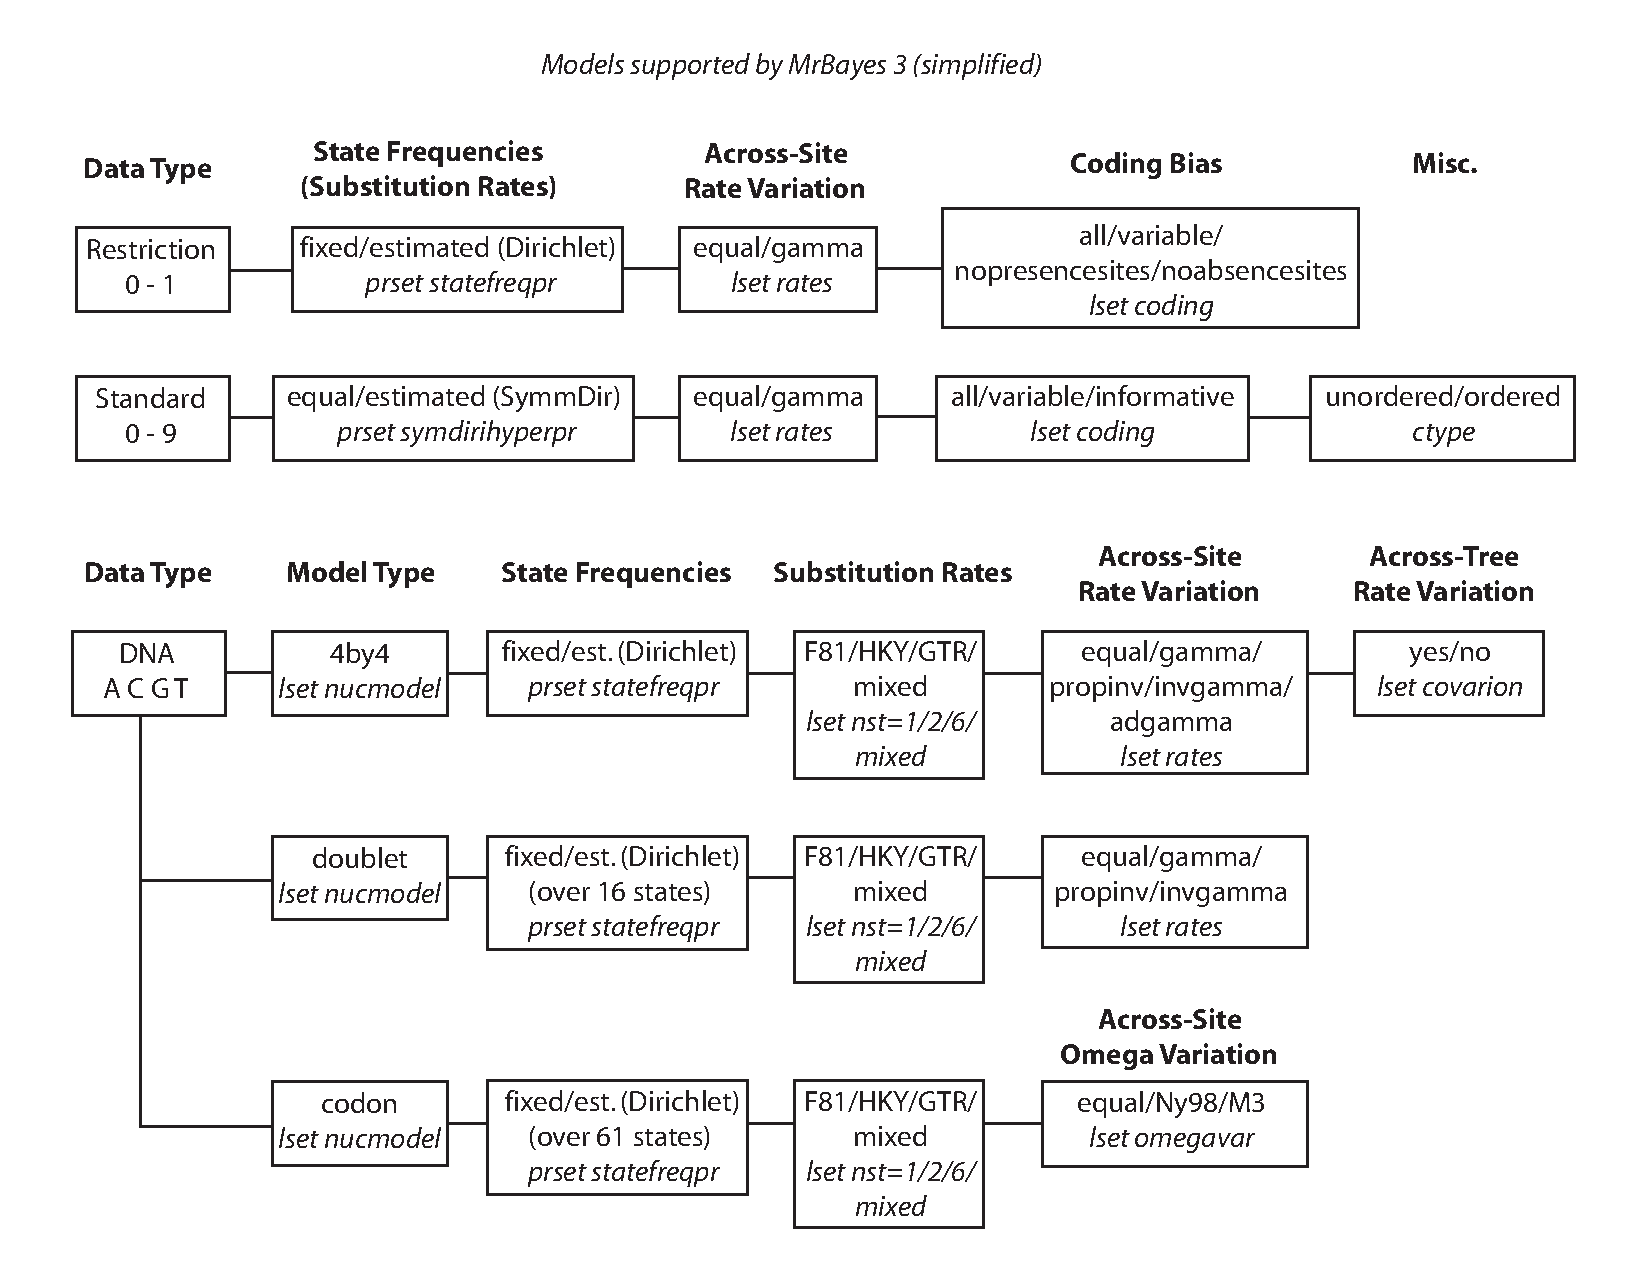
\includegraphics[angle=90,width=418pt]{Appendix_Fig1.pdf}
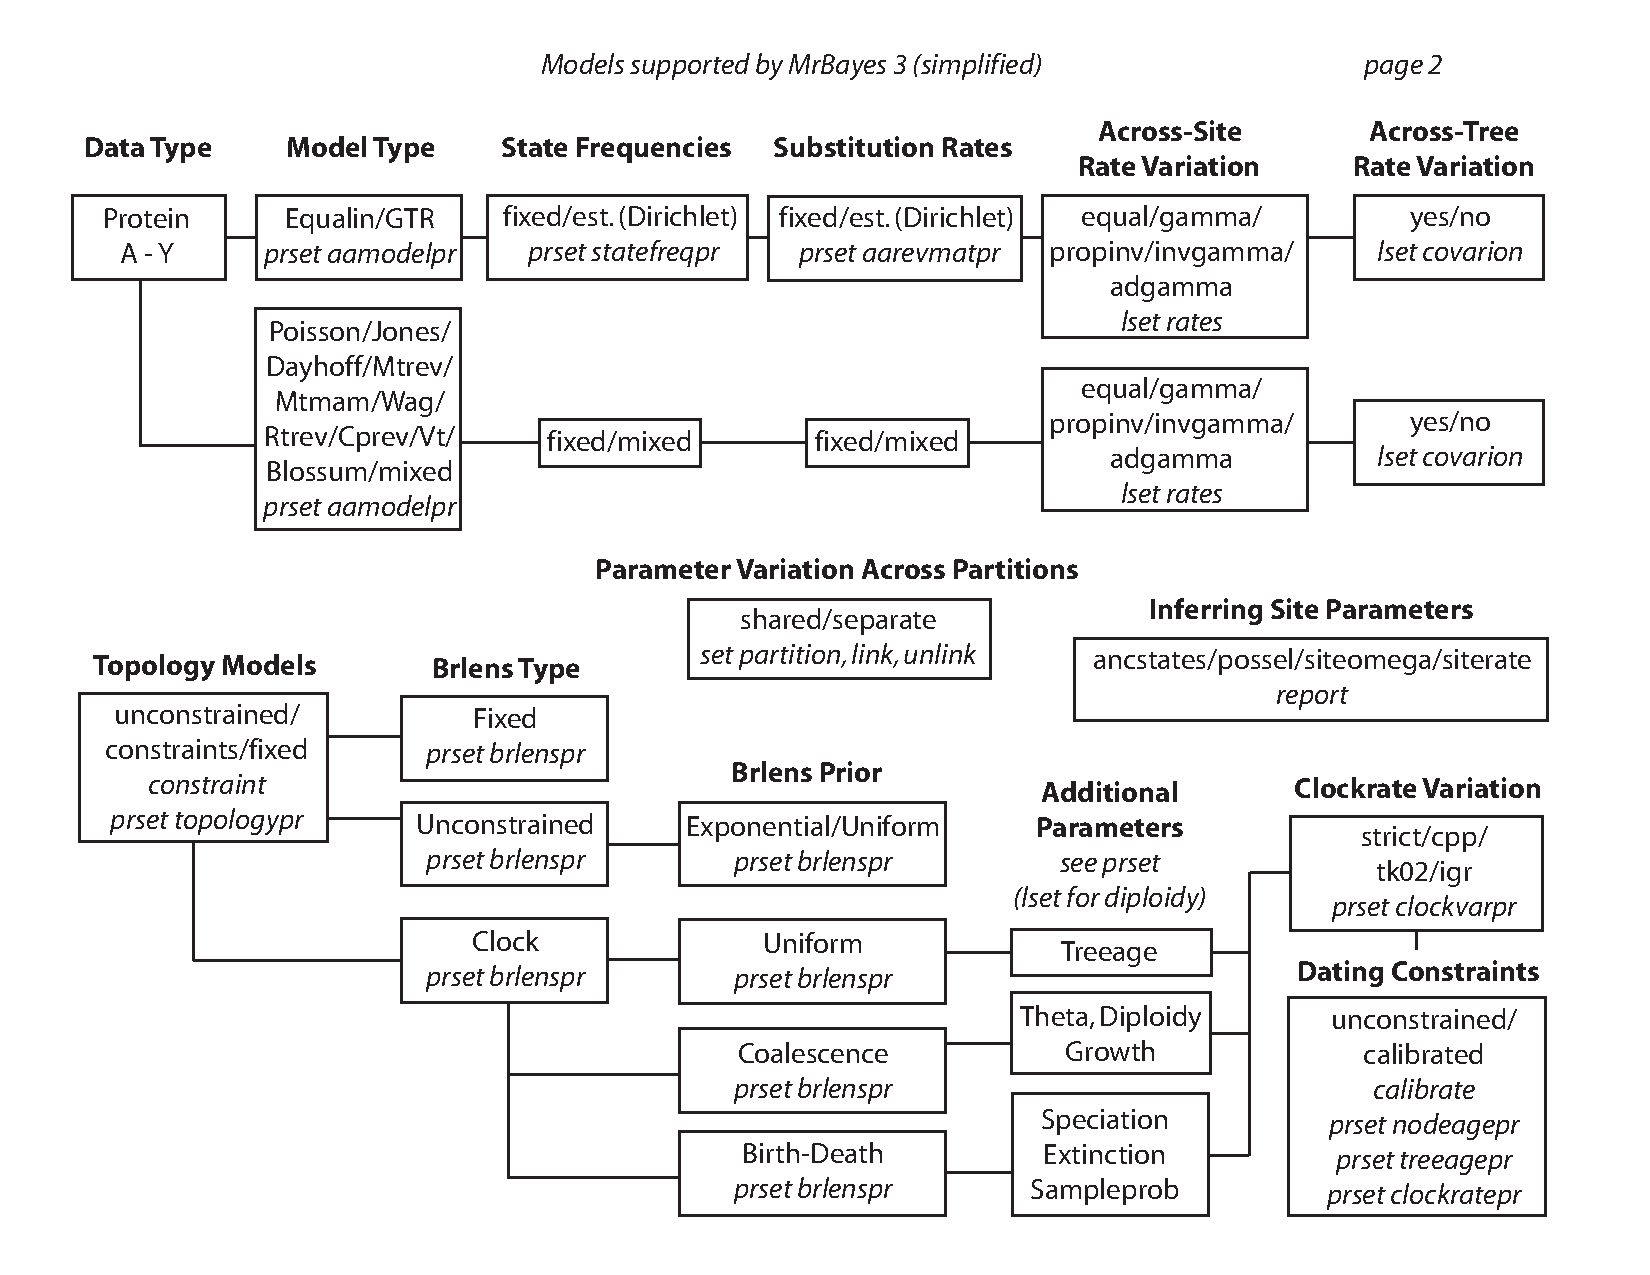
\includegraphics[angle=90,width=418pt]{Appendix_Fig2.pdf}
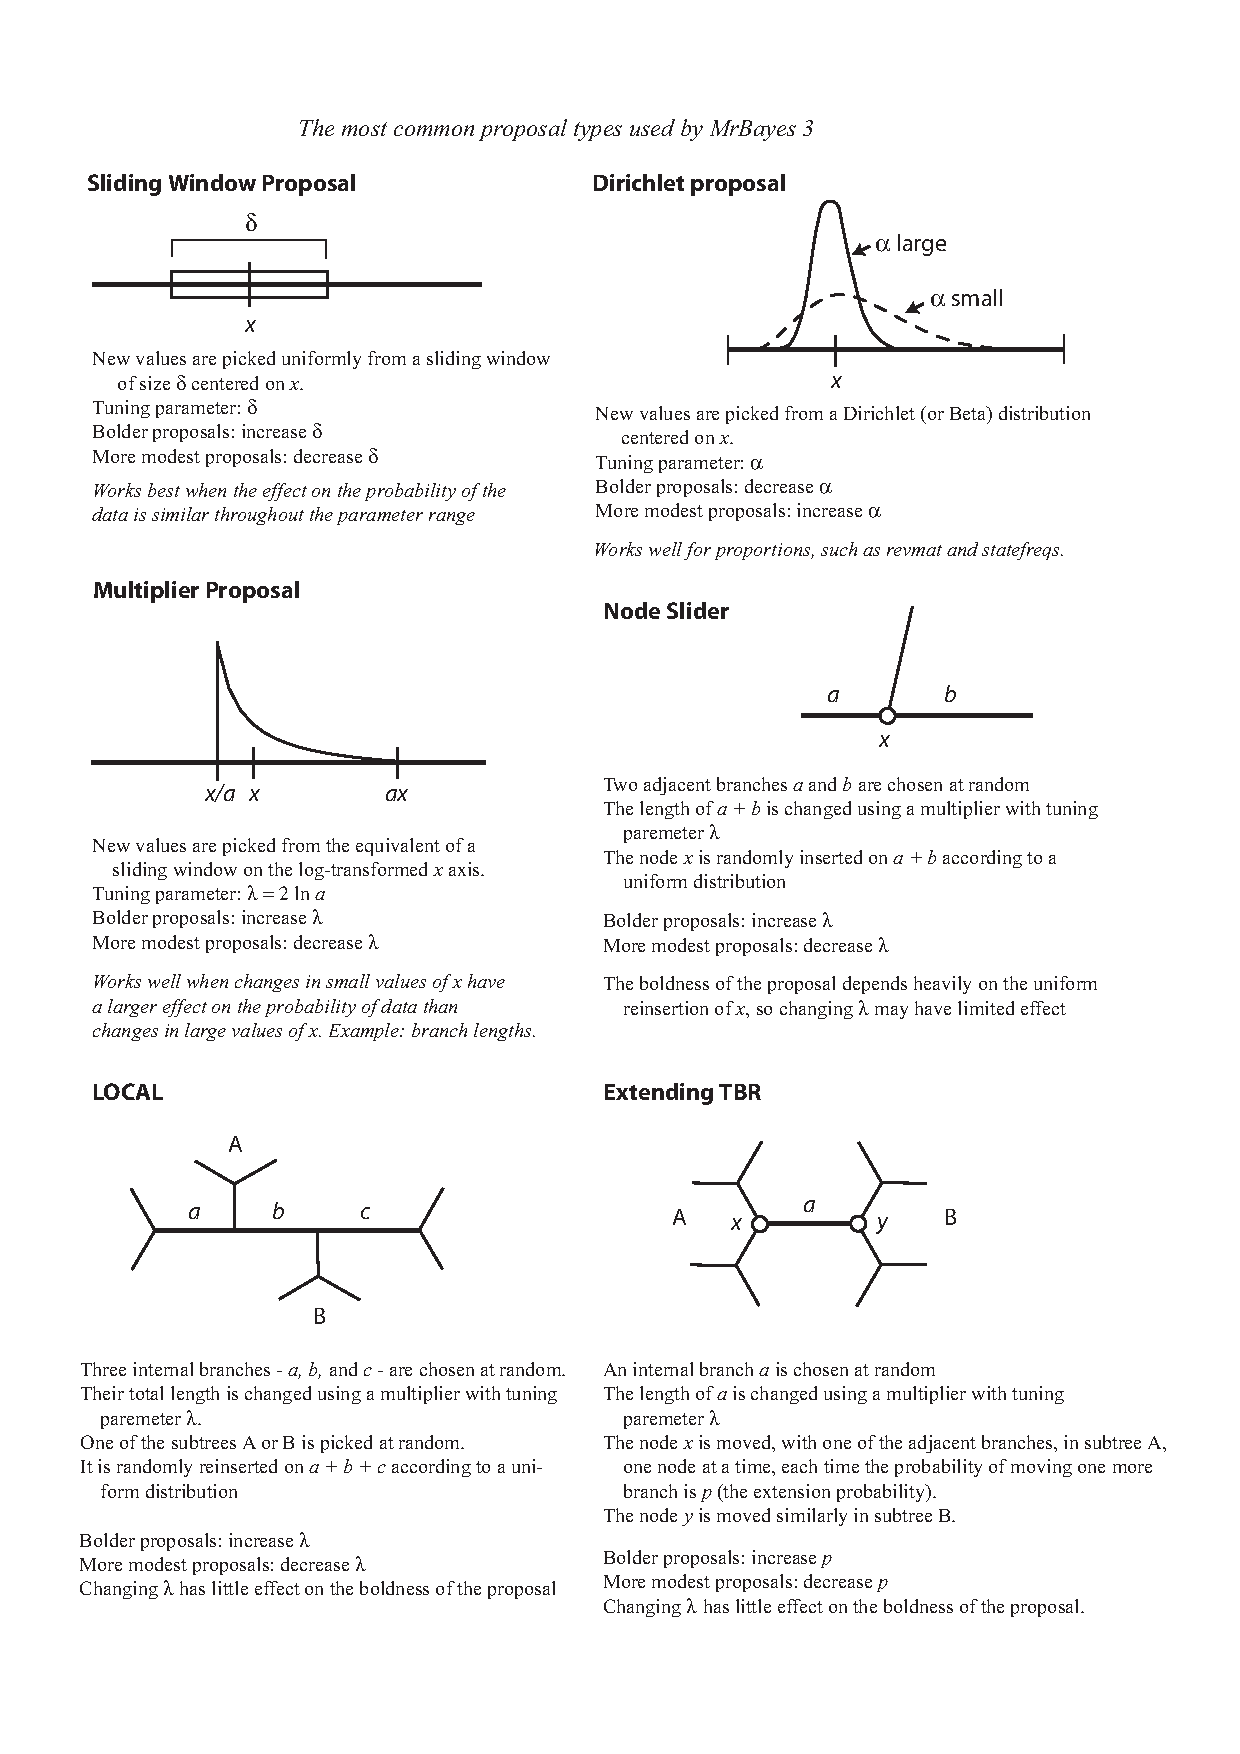
\includegraphics[width=418pt]{Appendix_Fig3.pdf}
%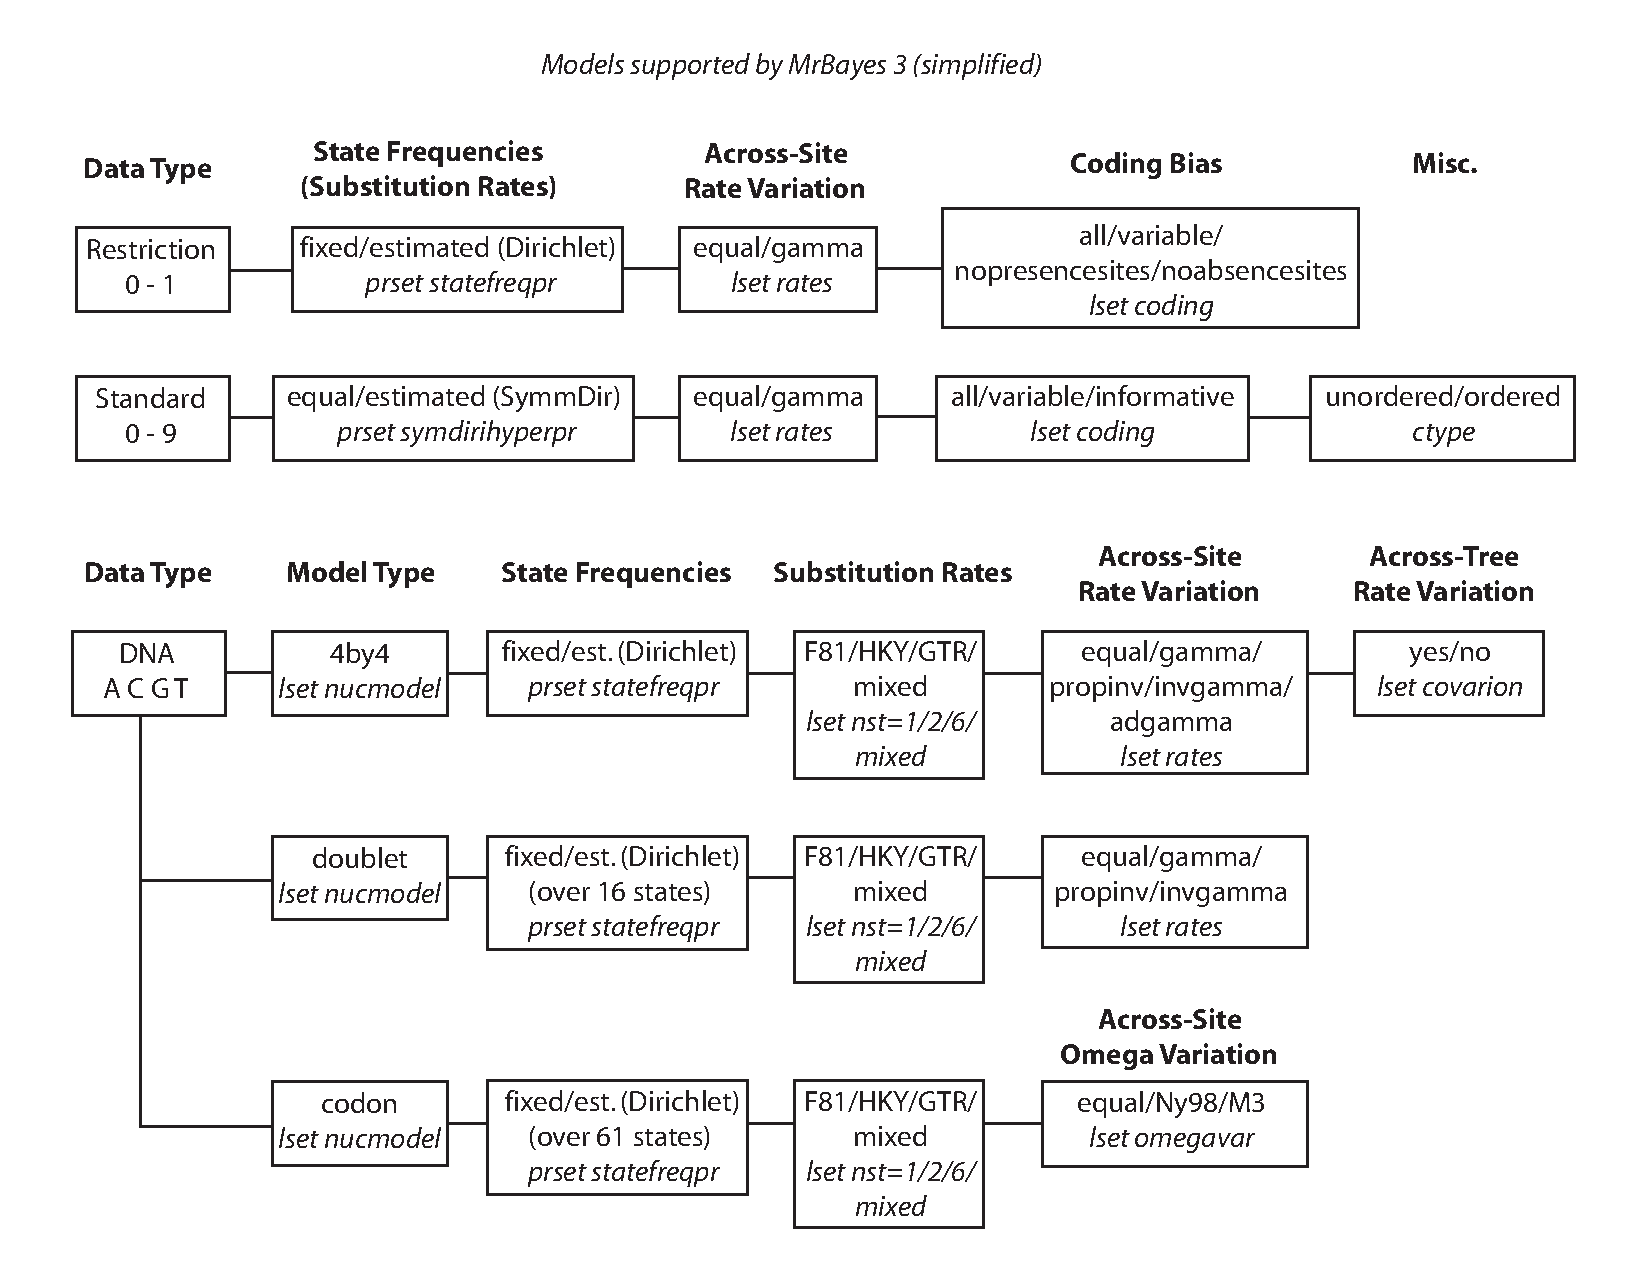
\includepdf[landscape=true]{Appendix_Fig1.pdf}
%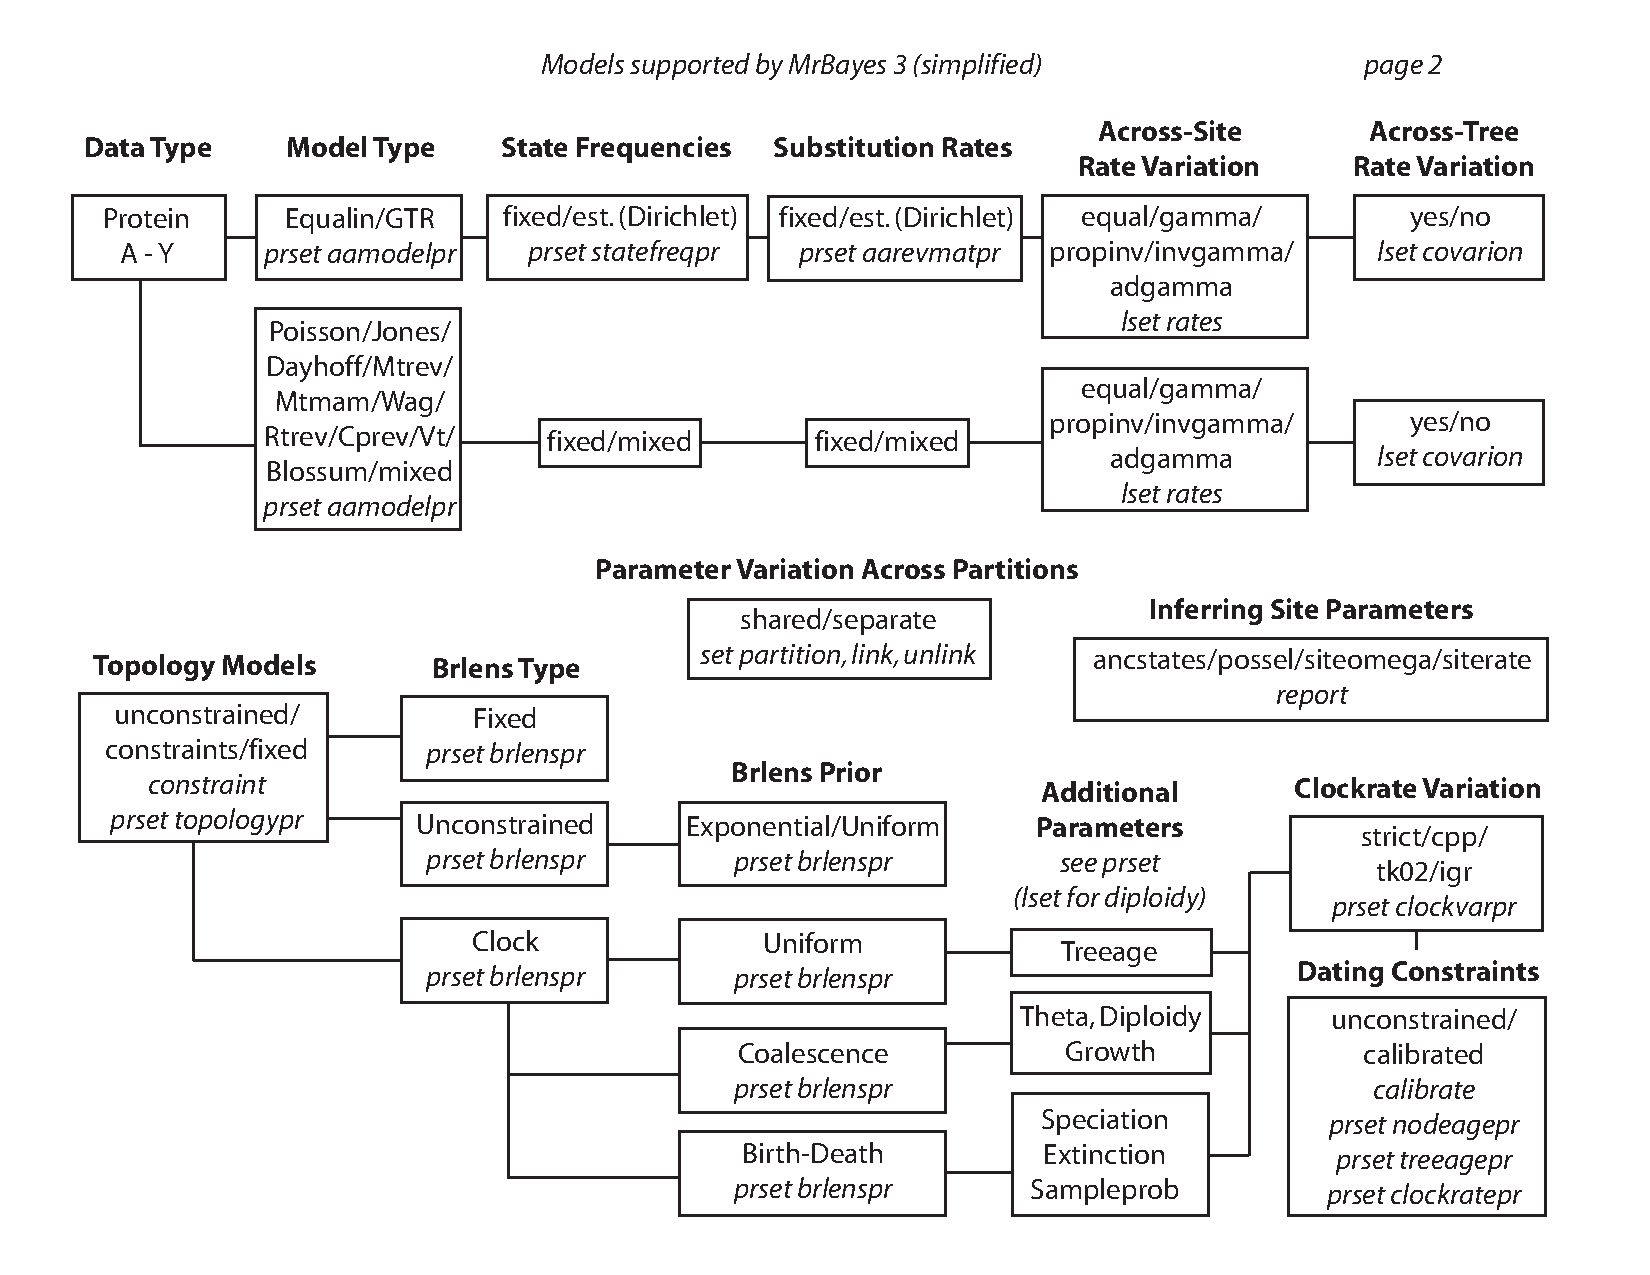
\includepdf[landscape=true]{Appendix_Fig2.pdf}
%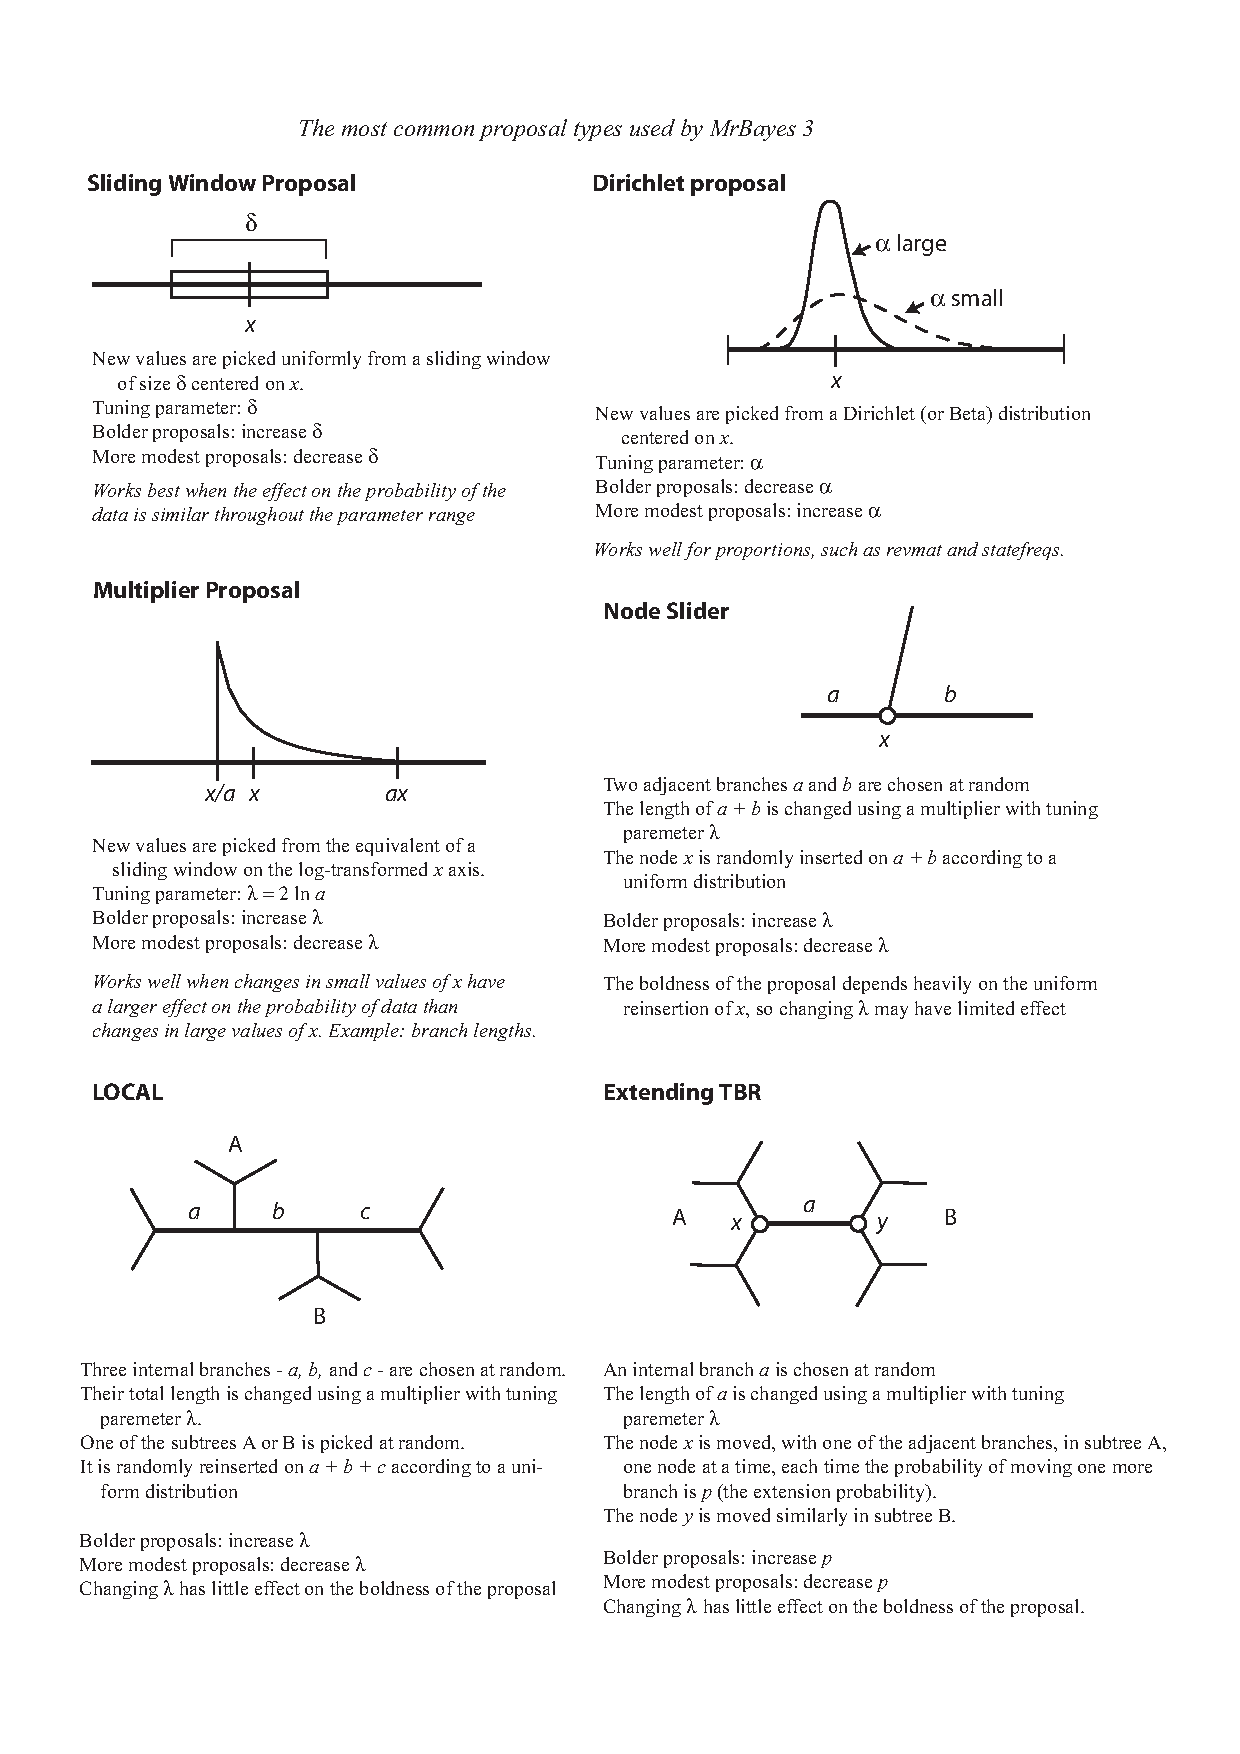
\includepdf[]{Appendix_Fig3.pdf}


%\bibliographystyle{alpha}	% or "unsrt", "alpha", "abbrv", etc.
\clearpage
\addcontentsline{toc}{chapter}{Bibliography}
\bibliographystyle{sysbio}
\bibliography{bayes}
\end{document}
